% LaTeX source for textbook ``The Little Book of Semaphores, 2nd edition''
% Copyright 2008 Allen B. Downey.

% Permission is granted to copy, distribute and/or modify this
% document under the terms of the GNU Free Documentation License,
% Version 1.1  or any later version published by the Free Software
% Foundation; with the Invariant Sections being "Contributor List",
% with no Front-Cover Texts, and with no Back-Cover Texts. A copy of
% the license is included in the section entitled "GNU Free
% Documentation License".

% You can obtain a copy of the GNU Free Documentation License
% from www.gnu.org or by writing to the Free Software Foundation,
% Inc., 59 Temple Place - Suite 330, Boston, MA 02111-1307, USA.
%
\documentclass{book}
\usepackage{fancyhdr}
\usepackage{listings}
\usepackage{graphicx}
\usepackage{color}
\usepackage{url}
\usepackage{makeidx}

\usepackage[colorlinks=true, linkcolor=blue, urlcolor=blue]{hyperref}

\title{The Little Book of Semaphores}

\author{Allen B. Downey}

\newcommand{\theversion}{Version 2.2.0}

\sloppy

\newcommand{\clearemptydoublepage}{\newpage\cleardoublepage}
\newcommand{\blankpage}{\newpage}

\pagestyle{fancyplain}

\renewcommand{\chaptermark}[1]{\markboth{#1}{}}
\renewcommand{\sectionmark}[1]{\markright{\thesection\ #1}{}}

\lhead[\fancyplain{}{\bfseries\thepage}]%
      {\fancyplain{}{\bfseries\rightmark}}
\rhead[\fancyplain{}{\bfseries\leftmark}]%
      {\fancyplain{}{\bfseries\thepage}}
\cfoot{}

% Commands that control the appearance of the listings
\definecolor{light-gray}{gray}{0.95}

\lstset{basicstyle=\tt, frame=single, 
backgroundcolor=\color{light-gray}, escapeinside={(*}{*)},
numbers=left, numberstyle=\tiny, numbersep=10pt}

\makeindex

\begin{document}
\title {The Little Book of Semaphores}
\author {Allen B. Downey}

\date {\theversion}
\maketitle

\vspace{2in}
\begin{center}
{\Large The Little Book of Semaphores}

Second Edition
\vspace{0.25in}

\theversion
\vspace{0.25in}

Copyright 2011 Allen B. Downey
\end{center}
\vspace{0.25in}

Permission is granted to copy, distribute and/or modify this
document under the terms of the GNU Free Documentation License,
Version 1.1  or any later version published by the Free Software
Foundation; this book contains no Invariant Sections,
no Front-Cover Texts, and no Back-Cover Texts.

You can obtain a copy of the GNU Free Documentation License
from www.gnu.org or by writing to the Free Software Foundation,
Inc., 59 Temple Place - Suite 330, Boston, MA 02111-1307, USA.

The original form of this book is LaTeX source code.
Compiling this LaTeX source has the effect of generating
a device-independent representation of a book, which
can be converted to other formats and printed.

This book was typeset by the author using latex, dvips and ps2pdf,
among other free, open-source programs.
The LaTeX source for this book is available from
\url{http://greenteapress.com/semaphores}.

\frontmatter

\chapter{Preface}

Most undergraduate Operating Systems textbooks have a module on
Synchronization, which usually presents a set of primitives
(mutexes, semaphores, monitors, and sometimes condition variables),
and classical problems like readers-writers and
producers-consumers.

When I took the Operating Systems class at Berkeley, and taught it at
Colby College, I got the impression that most students were able to
understand the solutions to these problems, but few would have been
able to produce them, or solve similar problems.

One reason students don't understand this material deeply is that
it takes more time, and more practice, than most classes can spare.
Synchronization is just one of the modules competing for space in
an Operating Systems class, and I'm not sure I can argue that it is
the most important.  But I do think it is one of the most challenging,
interesting, and (done right) fun.

I wrote the first edition this book with the goal of identifying
synchronization idioms and patterns that could be 
understood in isolation and then assembled to solve complex problems.
This was a challenge, because synchronization code doesn't compose
well; as the number of components increases, the number of interactions
grows unmanageably.

Nevertheless, I found patterns in the solutions I saw, and discovered
at least some systematic approaches to assembling solutions that are
demonstrably correct.

I had a chance to test this approach when I taught Operating Systems
at Wellesley College.  I used the first edition of {\em The Little
Book of Semaphores} along with one of the standard textbooks, and I
taught Synchronization as a concurrent thread for the duration of the
course.  Each week I gave the students a few pages from the book,
ending with a puzzle, and sometimes a hint.  I told them not to look
at the hint unless they were stumped.

I also gave them some tools for testing their solutions: a small
magnetic whiteboard where they could write code, and a stack of
magnets to represent the threads executing the code.

The results were dramatic.  Given more time to absorb the material,
students demonstrated a depth of understanding I had not seen before.
More importantly, most of them were able to solve most of the puzzles.
In some cases they reinvented classical solutions; in other cases
they found creative new approaches.

When I moved to Olin College, I took the next step and created a
half-class, called Synchronization, which covered
{\em The Little Book of Semaphores} and also the implementation of
synchronization primitives in x86 Assembly Language, POSIX, and
Python.

The students who took the class
helped me find errors in the first edition and several
of them contributed solutions that were better than mine.  At the
end of the semester, I asked each of them to write a new,
original problem (preferably with a solution).  I have added their
contributions to the second edition.

Also since the first edition appeared, Kenneth Reek presented the
article ``Design Patterns for Semaphores'' at the ACM Special Interest
Group for Computer Science Education.  He presents a problem, which
I have cast as the Sushi Bar Problem, and two solutions that demonstrate
patterns he calls ``Pass the baton'' and ``I'll do it for you.''
Once I came to appreciate these patterns, I was able to apply them
to some of the problems from the first edition and produce solutions
that I think are better.

One other change in the second edition is the syntax.  After I wrote
the first edition, I learned Python, which is not only a great
programming language; it also makes a great pseudocode language.  So I
switched from the C-like syntax in the first edition to syntax
that is pretty close to executable Python\footnote{The primary
difference is that I sometimes use indentation to indicate code that
is protected by a mutex, which would cause syntax errors in Python.}.
In fact, I have written a simulator that can execute many of the
solutions in this book.

Readers who are not familiar with Python will (I hope) find it mostly
obvious.  In cases where I use a Python-specific feature, I explain the
syntax and what it means.  I hope that these changes make the book
more readable.

The pagination of this book might seem peculiar, but there is a method
to my whitespace.  After each puzzle, I leave enough space that the
hint appears on the next sheet of paper and the solution on the next
sheet after that.  When I use this book in my class, I hand it out a
few pages at a time, and students collect them in a binder.  My
pagination system makes it possible to hand out a problem without
giving away the hint or the solution.  Sometimes I fold and staple the
hint and hand it out along with the problem so that students can
decide whether and when to look at the hint.  If you print the book
single-sided, you can discard the blank pages and the system still
works.

This is a Free Book, which means that anyone is welcome to read,
copy, modify and redistribute it, subject to the restrictions of the
license, which is the GNU Free Documentation License.  I hope that people
will find this book useful, but I also hope they will help continue
to develop it by sending in corrections, suggestions, and additional
material.  Thanks!

\vspace{0.3in}

\noindent Allen B. Downey \\
\noindent Needham, MA \\
\noindent June 1, 2005 \\


\section*{Contributor's list}

The following are some of the people who have contributed to this
book:

\begin{itemize}

\item Many of the problems in this book are variations of classical
problems that appeared first in technical articles and then in textbooks.
Whenever I know the origin of a problem or solution, I acknowledge it
in the text.

\item I also thank the students at Wellesley College who worked with
the first edition of the book, and the students at Olin College who
worked with the second edition.

\item Se Won sent in a small but important correction in my presentation
of Tanenbaum's solution to the Dining Philosophers Problem.

\item Daniel Zingaro punched a hole in the Dancer's problem, which
provoked me to rewrite that section.  I can only hope that it makes more
sense now.  Daniel also pointed out an error in a previous version of
my solution to the H$_2$O problem, and then wrote back a year later
with some typos.

\item Thomas Hansen found a typo in the Cigarette smokers problem.

\item Pascal R\"{u}tten pointed out several typos, including my embarrassing
misspelling of Edsger Dijkstra.

\item Marcelo Johann pointed out an error in my solution to the
Dining Savages problem, and fixed it!

\item Roger Shipman sent a whole passel of corrections as well as
an interesting variation on the Barrier problem.

\item Jon Cass pointed out an omission in the discussion of dining
philosophers.

\item Krzysztof Ko\'{s}ciuszkiewicz sent in several corrections, including
a missing line in the Fifo class definition.

\item Fritz Vaandrager at the Radboud University Nijmegen in the
Netherlands and his students Marc Schoolderman, Manuel Stampe and Lars
Lockefeer used a tool called UPPAAL to check several of the solutions
in this book and found errors in my solutions to the Room Party problem
and the Modus Hall problem.

\item Eric Gorr pointed out an explanation in Chapter 3 that was
not exactly right.

\item Jouni Lepp\"{a}j\"{a}rvi helped clarify the origins of semaphores.

\item Christoph Bartoschek found an error in a solution to
the exclusive dance problem.

\item Eus found a typo in Chapter 3.

\item Tak-Shing Chan found an out-of-bounds error in {\tt counter\_mutex.c}.

\item Roman V. Kiseliov made several suggestions for improving
the appearance of the book, and helped me with some \LaTeX~issues.

\item Alejandro C\'{e}spedes is working on the Spanish translation of this
book and found some typos.

\item Erich Nahum found a problem in my adaptation of Kenneth Reek's
  solution to the Sushi Bar Problem.

\item Martin Storsj\"{o} sent a correction to the generalized smokers problem.

\item Cris Hawkins pointed out an unused variable.

\item Adolfo Di Mare found the missing ``and''.

\item Simon Ellis found a typo.

\item Benjamin Nash found a typo, an error in one solution, and
a malfeature in another.

\item Alejandro Pulver found a problem with the Barbershop solution.

\end{itemize}

% endcontrib

\tableofcontents
\clearemptydoublepage

\mainmatter


\chapter{Introduction}

\section{Synchronization}
\label{synch}

In common use, ``synchronization'' means making two things happen
at the same time.  In computer systems, synchronization is a little
more general; it refers to relationships among events---any number
of events, and any kind of relationship (before, during, after).

Computer programmers are often concerned with {\bf synchronization
constraints}, which are requirements pertaining to the order of
events.  Examples include:

\begin{description}

\item[Serialization:] Event A must happen before Event B.

\item[Mutual exclusion:] Events A and B must not happen at the same time.

\end{description}

In real life we often check and enforce synchronization constraints 
using a clock.  How do we know if A happened before B?  If we
know what time both events occurred, we can just compare the times.

In computer systems, we often need to satisfy synchronization
constraints without the benefit of a clock, either because there
is no universal clock, or because we don't know with fine enough
resolution when events occur.

That's what this book is about: software techniques for enforcing
synchronization constraints.


\section {Execution model}

In order to understand software synchronization, you have to
have a model of how computer programs run.  In the simplest
model, computers execute one instruction after another in
sequence.  In this model, synchronization is trivial; we can
tell the order of events by looking at the program.  If Statement
A comes before Statement B, it will be executed first.

There are two ways things get more complicated.  One possibility
is that the computer is parallel, meaning that it has multiple
processors running at the same time.  In that case it is not easy
to know if a statement on one processor is executed before a
statement on another.

Another possibility is that a single processor is running multiple
threads of execution.  A thread is a sequence of instructions
that execute sequentially.  If there are multiple threads, then
the processor can work on one for a while, then switch to
another, and so on.

In general the programmer has no control over when each thread runs;
the operating system (specifically, the scheduler) makes those
decisions.  As a result, again, the programmer can't tell when
statements in different threads will be executed.

For purposes of synchronization, there is no difference between the
parallel model and the multithread model.  The issue is the
same---within one processor (or one thread) we know the order of
execution, but between processors (or threads) it is impossible to
tell.

A real world example might make this clearer.  Imagine that you and
your friend Bob live in different cities, and one day, around dinner
time, you start to wonder who ate lunch first that day, you or Bob.
How would you find out?

Obviously you could call him and ask what time he ate lunch.  But what
if you started lunch at 11:59 by your clock and Bob started lunch at
12:01 by his clock?  Can you be sure who started first?  Unless you
are both very careful to keep accurate clocks, you can't.

Computer systems face the same problem because, even though their
clocks are usually accurate, there is always a limit to their
precision.  In addition, most of the time the computer does not keep
track of what time things happen.  There are just too many things
happening, too fast, to record the exact time of everything.

Puzzle: Assuming that Bob is willing to follow simple instructions, is
there any way you can {\em guarantee} that tomorrow you will eat lunch
before Bob?

\clearemptydoublepage
\section {Serialization with messages}
\label{serialization}

One solution is to instruct Bob not to eat lunch until you call.
Then, make sure you don't call until after lunch.  This approach may
seem trivial, but the underlying idea, message passing, is a real
solution for many synchronization problems.
At the risk of belaboring the obvious, consider this timeline.
%
\begin{minipage}[t]{2in}
\begin{lstlisting}[title={Thread A (You)}]{}
Eat breakfast 
Work          
Eat lunch     
Call Bob
\end{lstlisting}
\end{minipage}
\hfill
\begin{minipage}[t]{2in}
\begin{lstlisting}[title={Thread B (Bob)}]{}
Eat breakfast
Wait for a call
Eat lunch
\end{lstlisting}
\end{minipage}
%
The first column is a list of actions you perform; in other words,
your thread of execution.  The second column is Bob's thread of
execution.  Within a thread, we can always tell what order things
happen.  We can denote the order of events
%
\begin{eqnarray*}
a1 < a2 < a3 < a4  \\
b1 < b2 < b3
\end{eqnarray*}
%
where the relation $a1 < a2$ means that a1 happened before a2.

In general, though, there is no way to compare events from different
threads; for example, we have no idea who ate breakfast first (is $a1
< b1$?).

But with message passing (the phone call) we {\em can} tell who ate
lunch first ($a3 < b3$).  Assuming that Bob has no other friends, he
won't get a call until you call, so $b2 > a4$ .  Combining all the
relations, we get
%
\begin{eqnarray*}
b3 > b2 > a4 > a3
\end{eqnarray*}
%
which proves that you had lunch before Bob.

In this case, we would say that you and Bob ate lunch
{\bf sequentially}, because we know the order of events, and you
ate breakfast {\bf concurrently}, because we don't.

When we talk about concurrent events, it is tempting to say
that they happen at the same time, or simultaneously.  As a
shorthand, that's fine, as long as you remember the strict
definition:

\begin{quote}
Two events are concurrent if we cannot tell by looking at
the program which will happen first.
\end{quote}

Sometimes we can tell, after the program runs, which happened first,
but often not, and even if we can, there is no guarantee that we will
get the same result the next time.


\newpage
\section {Non-determinism}

Concurrent programs are often {\bf non-deterministic}, which means it
is not possible to tell, by looking at the program, what will happen
when it executes.  Here is a simple example of a
non-deterministic program:

\begin{minipage}[t]{2in}
\begin{lstlisting}[title={Thread A}]{}
print "yes"
\end{lstlisting}
\end{minipage}
\hfill
\begin{minipage}[t]{2in}
\begin{lstlisting}[title={Thread B}]{}
print "no"
\end{lstlisting}
\end{minipage}

Because the two threads run concurrently, the order of
execution depends on the scheduler.  During any given run
of this program, the output might be ``yes no'' or ``no yes''.

Non-determinism is one of the things that makes concurrent
programs hard to debug.  A program might work correctly
1000 times in a row, and then crash on the 1001st run, depending
on the particular decisions of the scheduler.

These kinds of bugs are almost impossible to find by testing;
they can only be avoided by careful programming.


\section {Shared variables}
\label{shared}

Most of the time, most variables in most threads are {\bf local},
meaning that they belong to a single thread and no other threads
can access them.  As long as that's true, there tend to be few
synchronization problems, because threads just don't interact.

But usually some variables are {\bf shared} among two or more
threads; this is one of the ways threads interact with each other.
For example, one way to communicate information between threads is
for one thread to read a value written by another thread.

If the threads are unsynchronized, then we cannot tell by looking at
the program whether the reader will see the value the writer writes
or an old value that was already there.
Thus many applications enforce the constraint that the reader
should not read until after the writer writes.  This is exactly
the serialization problem in Section~\ref{serialization}.

Other ways that threads interact are
concurrent writes (two or more writers) and concurrent updates
(two or more threads performing a read followed by a write).
The next two sections deal with these interactions.  The other
possible use of a shared variable, concurrent
reads, does not generally create a synchronization problem.


\subsection {Concurrent writes}

In the following example, {\tt x} is a shared variable accessed
by two writers.

\begin{minipage}[t]{2in}
\begin{lstlisting}[title={Thread A}]{}
x = 5
print x
\end{lstlisting}
\end{minipage}
\hfill
\begin{minipage}[t]{2in}
\begin{lstlisting}[title={Thread B}]{}
x = 7
\end{lstlisting}
\end{minipage}

What value of {\tt x} gets printed?  What is the final value of {\tt
x} when all these statements have executed?  It depends on the order
in which the statements are executed, called the {\bf execution path}.
One possible path is $a1 < a2 < b1$, in which case the output of the
program is {\tt 5}, but the final value is {\tt 7}.

Puzzle: What path yields output {\tt 5} and final
value {\tt 5}?

Puzzle: What path yields output {\tt 7} and final
value {\tt 7}?

Puzzle: Is there a path that yields output {\tt 7} and final
value {\tt 5}?  Can you prove it?

Answering questions like these is an important part of concurrent
programming:  What paths are possible and what are the
possible effects?  Can we prove that a given (desirable) effect is
necessary or that an (undesirable) effect is impossible?


\subsection {Concurrent updates}

An update is an operation that reads the value of a variable, computes
a new value based on the old value, and writes the new value.
The most common kind of update is an increment, in which the
new value is the old value plus one.  The following example
shows a shared variable, {\tt count}, being updated concurrently
by two threads.

\begin{minipage}[t]{2in}
\begin{lstlisting}[title={Thread A}]{}
count = count + 1
\end{lstlisting}
\end{minipage}
\hfill
\begin{minipage}[t]{2in}
\begin{lstlisting}[title={Thread B}]{}
count = count + 1
\end{lstlisting}
\end{minipage}

At first glance, it is not obvious that there is a synchronization
problem here.  There are only two execution paths, and they
yield the same result.

The problem is that these operations are translated into
machine language before execution, and in machine language
the update takes two steps, a read and a write.
The problem is more obvious if we rewrite the code with a temporary
variable, {\tt temp}.

\begin{minipage}[t]{2in}
\begin{lstlisting}[title={Thread A}]{}
temp = count
count = temp + 1
\end{lstlisting}
\end{minipage}
\hfill
\begin{minipage}[t]{2in}
\begin{lstlisting}[title={Thread B}]{}
temp = count
count = temp + 1
\end{lstlisting}
\end{minipage}

Now consider the following execution path 

\[  a1 < b1 < b2 < a2  \]

Assuming that the
initial value of {\tt x} is {\tt 0},
what is its final value?  Because
both threads read the same initial value, they write
the same value.  The variable is only incremented once, which
is probably not what the programmer had in mind.

This kind of problem is subtle because it is not always possible to
tell, looking at a high-level program, which operations are
performed in a single step and which can be interrupted.
In fact, some computers provide an increment instruction that
is implemented in hardware and cannot be interrupted.
An operation that cannot be interrupted is said to be
{\bf atomic}.

So how can we write concurrent programs if we don't know which
operations are atomic?  One possibility is to collect specific
information about each operation on each hardware platform.
The drawbacks of this approach are obvious.

The most common alternative is to make the conservative
assumption that all updates and all writes are not atomic,
and to use synchronization constraints to control concurrent
access to shared variables.

The most common constraint is mutual exclusion, or mutex,
which I mentioned in Section~\ref{synch}.  Mutual exclusion guarantees
that only one thread accesses a shared variable at a time,
eliminating the kinds of synchronization errors in this section.

Puzzle: Suppose that 100 threads run the following program concurrently
(if you are not familiar with Python, the {\tt for} loop runs the update
100 times.):

\begin{lstlisting}[]{}
for i in range(100):
    temp = count
    count = temp + 1
\end{lstlisting}

What is the largest possible value of {\tt count} after all threads
have completed?  What is the smallest possible value?

Hint: the first question is easy; the second is not.

\subsection {Mutual exclusion with messages}

Like serialization, mutual exclusion
can be implemented using message passing.  For example, imagine that
you and Bob operate a nuclear reactor that you monitor from remote
stations.  Most of the time, both of you are watching for warning
lights, but you are both allowed to take a break for lunch.  It
doesn't matter who eats lunch first, but it is very important that
you don't eat lunch at the same time, leaving the reactor unwatched!

Puzzle: Figure out a system of message passing (phone calls) that
enforces these restraints.  Assume there are no clocks, and you
cannot predict when lunch will start or how long it will last.  What
is the minimum number of messages that is required?


\clearemptydoublepage
\chapter{Semaphores}

In real life a semaphore is a system of signals used to communicate
visually, usually with flags, lights, or some other mechanism.  In
software, a semaphore is a data structure that is useful for solving a
variety of synchronization problems.

Semaphores were invented by Edsger Dijkstra, a famously eccentric
computer scientist.  Some of the details have changed since the
original design, but the basic idea is the same.

\section{Definition}

A semaphore is like an integer, with three differences:

\begin{enumerate}

\item When you create the semaphore, you can initialize its value to
any integer, but after that the only operations you are allowed to
perform are increment (increase by one) and decrement (decrease by
one).  You cannot read the current value of the semaphore.

\item When a thread decrements the semaphore, if the result is
negative, the thread blocks itself and cannot continue until another
thread increments the semaphore.

\item When a thread increments the semaphore, if there are other
threads waiting, one of the waiting threads gets unblocked.

\end{enumerate}

To say that a thread blocks itself (or simply ``blocks'') is to say
that it notifies the scheduler that it cannot proceed.  The scheduler
will prevent the thread from running until an event occurs that causes
the thread to become unblocked.  In the tradition of mixed metaphors
in computer science, unblocking is often called ``waking''.

That's all there is to the definition, but there are some
consequences of the definition you might want to think about.

\begin{itemize}

\item In general, there is no way to know before a thread decrements a
semaphore whether it will block or not (in specific cases you might
be able to prove that it will or will not).

\item After a thread increments a semaphore and another thread gets
woken up, both threads continue running concurrently.  There is no way
to know which thread, if either, will continue immediately.

\item When you signal a semaphore, you don't necessarily know whether
another thread is waiting, so the number of unblocked threads may
be zero or one.

\end{itemize}

Finally, you might want to think about what the value of the
semaphore means.  If the value is positive, then it represents the
number of threads that can decrement without blocking.  If it
is negative, then it represents the number of threads that have
blocked and are waiting.  If the value is zero, it means there
are no threads waiting, but if a thread tries to decrement, it
will block.


\section{Syntax}

In most programming environments, an implementation of semaphores is
available as part of the programming language or the operating system.
Different implementations sometimes offer slightly different
capabilities, and usually require different syntax.

In this book I will use a simple pseudo-language to demonstrate
how semaphores work.  The syntax for creating a new semaphore
and initializing it is
%
\begin{lstlisting}[title={Semaphore initialization syntax}]{}
fred = Semaphore(1)
\end{lstlisting}
%
The function {\tt Semaphore} is a constructor; it creates and
returns a new Semaphore.  The initial value of the semaphore
is passed as a parameter to the constructor.

The semaphore operations go by different names in different environments.
The most common alternatives are 
%
\begin{lstlisting}[title={Semaphore operations}]{}
fred.increment()
fred.decrement()	
\end{lstlisting}
%
and
%
\begin{lstlisting}[title={Semaphore operations}]{}
fred.signal()
fred.wait()	
\end{lstlisting}
%
and
%
\begin{lstlisting}[title={Semaphore operations}]{}
fred.V()
fred.P()	
\end{lstlisting}
%
It may be surprising that there are so many names, but there is a
reason.  {\tt increment} and {\tt decrement}
describe what the operations {\em do}.  {\tt signal} and {\tt wait}
describe what they are often {\em used for}.  And {\tt V} and {\tt P} were
the original names proposed by Dijkstra, who wisely realized that a
meaningless name is better than a misleading name\footnote{If you speak
Dutch, {\tt V} and {\tt P} aren't completely meaningless.}.

I consider the other pairs misleading because {\tt increment} and {\tt
decrement} neglect to mention the possibility of blocking and waking,
and semaphores are often used in ways that have nothing to do with
{\tt signal} and {\tt wait}.

If you insist on meaningful names, then I would suggest these:

\begin{lstlisting}[title={Semaphore operations}]{}
fred.increment_and_wake_a_waiting_process_if_any()
fred.decrement_and_block_if_the_result_is_negative()	
\end{lstlisting}

I don't think the world is likely to embrace either of these names
soon.  In the meantime, I choose (more or less arbitrarily) to use
{\tt signal} and {\tt wait}.


\section{Why semaphores?}

Looking at the definition of semaphores, it is not at all obvious why
they are useful.  It's true that we don't {\em need} semaphores to
solve synchronization problems, but there are some advantages to using
them:

\begin{itemize}

\item Semaphores impose deliberate constraints that help
programmers avoid errors.

\item Solutions using semaphores are often clean and organized,
making it easy to demonstrate their correctness.

\item Semaphores can be implemented efficiently on many systems,
so solutions that use semaphores are portable and usually
efficient.

\end{itemize}

\clearemptydoublepage
\chapter{Basic synchronization patterns}

This chapter presents a series of basic synchronization problems and
shows ways of using semaphores to solve them.  These problems include
serialization and mutual exclusion, which we have already seen, along
with others.

\section{Signaling}

Possibly the simplest use for a semaphore is {\bf signaling},
which means that one thread sends a signal to another
thread to indicate that something has happened.

Signaling makes it possible to guarantee
that a section of code in one thread will run before a section of
code in another thread; in other words, it solves the serialization
problem.

Assume that we have a semaphore named {\tt sem} with initial value
0, and that Threads A and B have shared access to it.

\begin{minipage}[t]{2in}
\begin{lstlisting}[title={Thread A}]{}
statement a1
sem.signal()
\end{lstlisting}
\end{minipage}
\hfill
\begin{minipage}[t]{2in}
\begin{lstlisting}[title={Thread B}]{}
sem.wait()
statement b1
\end{lstlisting}
\end{minipage}

The word {\tt statement} represents an arbitrary program statement.
To make the example concrete, imagine that {\tt a1} reads a line
from a file, and {\tt b1} displays the line on the screen.
The semaphore in this program guarantees that Thread A
has completed {\tt a1} before Thread B begins {\tt b1}.

Here's how it works: if thread B gets to the
{\tt wait} statement first, it will find the initial
value, zero, and it will block.  Then when Thread A signals,
Thread B proceeds.

Similarly, if Thread A gets to the signal first then the
value of the semaphore will be incremented, and when Thread
B gets to the wait, it will proceed immediately.
Either way, the order of {\tt a1} and {\tt b1} is guaranteed.

This use of semaphores is the basis of the names {\tt signal}
and {\tt wait}, and in this case the names are conveniently
mnemonic.  Unfortunately, we will see other cases where the
names are less helpful.

Speaking of meaningful names, {\tt sem} isn't one.  When
possible, it is a good idea to give a semaphore a name
that indicates what it represents.  In this case a name like
{\tt a1Done} might be good, so that {\tt a1done.signal()} means
``signal that a1 is done,'' and {\tt a1done.wait()} means
``wait until a1 is done.''


\section{Rendezvous}
\label{rendezvous}

Puzzle: Generalize the signal pattern so that it works both
ways.  Thread A has to wait for Thread B and vice versa.  In other
words, given this code

\begin{minipage}[t]{2in}
\begin{lstlisting}[title={Thread A}]{}
statement a1
statement a2
\end{lstlisting}
\end{minipage}
\hfill
\begin{minipage}[t]{2in}
\begin{lstlisting}[title={Thread B}]{}
statement b1
statement b2
\end{lstlisting}
\end{minipage}
%
we want to guarantee that {\tt a1} happens before {\tt b2} and
{\tt b1} happens before {\tt a2}.  In writing your solution, be sure
to specify the names and initial values of your semaphores
(little hint there).

Your solution should not enforce too many constraints.  For example,
we don't care about the order of {\tt a1} and {\tt b1}.  In your
solution, either order should be possible.

This synchronization problem has a name; it's a
rendezvous.  The idea is that two threads rendezvous
at a point of execution, and neither is allowed to proceed
until both have arrived.

\clearemptydoublepage
\subsection{Rendezvous hint}

The chances are good that you were able to figure out a solution,
but if not, here is a hint.  Create two semaphores, named {\tt aArrived}
and {\tt bArrived}, and initialize them both to zero.

As the names suggest, {\tt aArrived} indicates whether Thread A
has arrived at the rendezvous, and {\tt bArrived} likewise.

\clearemptydoublepage
\subsection{Rendezvous solution}

Here is my solution, based on the previous hint:

\begin{minipage}[t]{2in}
\begin{lstlisting}[title={Thread A}]{}
statement a1
aArrived.signal()
bArrived.wait()
statement a2
\end{lstlisting}
\end{minipage}
\hfill
\begin{minipage}[t]{2in}
\begin{lstlisting}[title={Thread B}]{}
statement b1
bArrived.signal()
aArrived.wait()
statement b2
\end{lstlisting}
\end{minipage}

While working on the previous problem, you might have
tried something like this:

\begin{minipage}[t]{2in}
\begin{lstlisting}[title={Thread A}]{}
statement a1
bArrived.wait()
aArrived.signal()
statement a2
\end{lstlisting}
\end{minipage}
\hfill
\begin{minipage}[t]{2in}
\begin{lstlisting}[title={Thread B}]{}
statement b1
bArrived.signal()
aArrived.wait()
statement b2
\end{lstlisting}
\end{minipage}

This solution also works, although it is probably less
efficient, since it might have to switch between A and B
one time more than necessary.

If A arrives first, it waits for B.  When B arrives, it wakes
A and might proceed immediately to its {\tt wait} in which
case it blocks, allowing A to reach its {\tt signal}, after
which both threads can proceed.

Think about the other possible paths through this code and
convince yourself that in all cases neither thread can
proceed until both have arrived.

\subsection {Deadlock \#1}

Again, while working on the previous problem, you might have
tried something like this:

\begin{minipage}[t]{2in}
\begin{lstlisting}[title={Thread A}]{}
statement a1
bArrived.wait()
aArrived.signal()
statement a2
\end{lstlisting}
\end{minipage}
\hfill
\begin{minipage}[t]{2in}
\begin{lstlisting}[title={Thread B}]{}
statement b1
aArrived.wait()
bArrived.signal()
statement b2
\end{lstlisting}
\end{minipage}

If so, I hope you rejected it quickly, because it has a serious
problem.  Assuming that A arrives first, it will block at its
{\tt wait}.  When B arrives, it will also block, since A wasn't
able to signal {\tt aArrived}.  At this point, neither thread
can proceed, and never will.

This situation is called a {\bf deadlock} and, obviously, it is
not a successful solution of the synchronization problem.  In
this case, the error is obvious, but often the possibility of
deadlock is more subtle.  We will see more examples later.


\section{Mutex}

A second common use for semaphores is to enforce mutual exclusion.
We have already seen one use for mutual exclusion, controlling
concurrent access to shared variables.  The mutex guarantees
that only one thread accesses the shared variable at a time.

A mutex is like a token that passes from one thread to another,
allowing one thread at a time to proceed.  For example, in {\em The
Lord of the Flies} a group of children use a conch as a mutex.  In
order to speak, you have to hold the conch.  As long as only one child
holds the conch, only one can speak\footnote{Although this metaphor
is helpful for now, it can also be misleading, as you will see in
Section~\ref{water}}.

Similarly, in order for a thread to access a shared variable,
it has to ``get'' the mutex; when it is done, it ``releases''
the mutex.  Only one thread can hold the mutex at a time.

Puzzle: Add semaphores to the following example to
enforce mutual exclusion to the shared variable {\tt count}.

\begin{minipage}[t]{2in}
\begin{lstlisting}[title={Thread A}]{}
count = count + 1
\end{lstlisting}
\end{minipage}
\hfill
\begin{minipage}[t]{2in}
\begin{lstlisting}[title={Thread B}]{}
count = count + 1
\end{lstlisting}
\end{minipage}


\clearemptydoublepage
\subsection{Mutual exclusion hint}

Create a semaphore named {\tt mutex} that is initialized
to 1.  A value of one means that a thread may proceed and
access the shared variable; a value of zero means that it
has to wait for another thread to release the mutex.


\clearemptydoublepage
\subsection{Mutual exclusion solution}

Here is a solution:

\begin{minipage}[t]{2in}
\begin{lstlisting}[title={Thread A}]{}
mutex.wait()
    # critical section
    count = count + 1
mutex.signal()
\end{lstlisting}
\end{minipage}
\hfill
\begin{minipage}[t]{2in}
\begin{lstlisting}[title={Thread B}]{}
mutex.wait()
    # critical section
    count = count + 1
mutex.signal()
\end{lstlisting}
\end{minipage}

Since {\tt mutex} is initially 1, whichever thread gets to
the {\tt wait} first will be able to proceed immediately.
Of course, the act of waiting on the semaphore has the effect
of decrementing it, so the second thread to
arrive will have to wait until the first signals.

I have indented the update operation to show that it is contained
within the mutex.

In this example, both threads are running the same code.  This is
sometimes called a {\bf symmetric} solution.  If the threads have to
run different code, the solution is {\bf asymmetric}.  Symmetric
solutions are often easier to generalize.  In this case, the mutex
solution can handle any number of concurrent threads without
modification.  As long as every thread waits before 
performing an update and signals after, then no two threads
will access {\tt count} concurrently.

Often the code that needs to be protected is called the
{\bf critical section}, I suppose because it is critically
important to prevent concurrent access.

In the tradition of computer science and mixed metaphors, there
are several other ways people sometimes talk about mutexes.  In
the metaphor we have been using so far, the mutex is a token
that is passed from one thread to another.

In an alternative
metaphor, we think of the critical section as a room, and
only one thread is allowed to be in the room at a time.
In this metaphor, mutexes are called locks, and a thread
is said to lock the mutex before entering and unlock it while
exiting.  Occasionally, though, people mix the metaphors and
talk about ``getting'' or ``releasing'' a lock, which doesn't
make much sense.

Both metaphors are potentially useful and potentially misleading.
As you work on the next problem, try out both ways of thinking
and see which one leads you to a solution.


\section{Multiplex}

Puzzle: Generalize the previous solution so that it allows multiple
threads to run in the critical section at the same time, but it
enforces an upper limit on the number of concurrent threads.  In other
words, no more than {\tt n} threads can run in the critical section at
the same time.

This pattern is called a {\bf multiplex}.  In real life, the multiplex
problem occurs at busy nightclubs where there is a maximum number of
people allowed in the building at a time, either to maintain fire
safety or to create the illusion of exclusivity.

At such places a bouncer usually enforces the synchronization
constraint by keeping track of the number of people inside
and barring arrivals when the room is at capacity.  Then,
whenever one person leaves another is allowed to enter.

Enforcing this constraint with semaphores may sound difficult, but it
is almost trivial.


\clearemptydoublepage
\subsection{Multiplex solution}

To allow multiple threads to run in the critical section, just
initialize the semaphore to {\tt n}, which is the maximum number
of threads that should be allowed.

At any time, the value of the semaphore represents the
number of additional threads that may enter.  If the value is zero,
then the next thread will block until one of the threads inside
exits and signals.  When all threads have exited the value of the
semaphore is restored to {\tt n}.

Since the solution is symmetric, it's conventional to show only one
copy of the code, but you should imagine multiple copies of the code
running concurrently in multiple threads.

\begin{lstlisting}[title={Multiplex solution}]{}
multiplex.wait()
    critical section 
multiplex.signal()      
\end{lstlisting}

What happens if the critical section is occupied and more than one
thread arrives?  Of course, what we want is for all the arrivals to
wait.  This solution does exactly that.  Each time an arrival joins
the queue, the semaphore is decremented, so that the value of the
semaphore (negated) represents the number of threads in queue.

When a thread leaves, it signals the semaphore, incrementing
its value and allowing one of the waiting threads to proceed.

Thinking again of metaphors, in this case I find it useful
to think of the semaphore as a set of tokens (rather than
a lock).
As each thread invokes {\tt wait}, it picks up one of
the tokens; when it invokes {\tt signal} it releases one.
Only a thread that holds a token can enter the room.  If no
tokens are available when a thread arrives, it waits until
another thread releases one.

In real life, ticket windows sometimes use a system like
this.  They hand out tokens (sometimes poker chips) to
customers in line.  Each token allows the holder to buy a ticket.




\section{Barrier}

Consider again the Rendezvous problem from Section~\ref{rendezvous}.
A limitation of the solution we presented is that it does
not work with more than two threads.

Puzzle: Generalize the rendezvous solution.  Every thread should
run the following code:

\begin{lstlisting}[title={Barrier code}]{}
rendezvous
critical point
\end{lstlisting}

The synchronization requirement is that
no thread executes {\tt critical point} until after all
threads have executed {\tt rendezvous}.

You can assume that there are $n$
threads and that this value is stored in a variable, {\tt n},
that is accessible from all threads.

When the first $n-1$ threads arrive they should block until the $n$th
thread arrives, at which point all the threads may proceed.


\clearemptydoublepage
\subsection {Barrier hint}

For many of the problems in this book I will provide hints
by presenting the variables I used in my solution and
explaining their roles.

\begin{lstlisting}[title={Barrier hint}]{}
n = the number of threads
count = 0
mutex = Semaphore(1)
barrier = Semaphore(0)
\end{lstlisting}

{\tt count} keeps track of how many threads have arrived.
{\tt mutex} provides exclusive access to {\tt count} so that
threads can increment it safely.

{\tt barrier} is locked
(zero or negative) until all threads arrive; then it should
be unlocked (1 or more).


\clearemptydoublepage
\subsection {Barrier non-solution}

First I will present a solution that is not quite right, because
it is useful to examine incorrect solutions and figure out what
is wrong.

\begin{lstlisting}[title={Barrier non-solution}]{}
rendezvous

mutex.wait()
    count = count + 1
mutex.signal()

if count == n: barrier.signal()

barrier.wait()

critical point
\end{lstlisting}

Since {\tt count} is protected by a mutex, it counts the number of
threads that pass.  The first $n-1$ threads wait when they get to the
barrier, which is initially locked.  When the $n$th thread arrives, it
unlocks the barrier.

Puzzle:  What is wrong with this solution?


\clearemptydoublepage
\subsection{Deadlock \#2}

The problem is a deadlock.

An an example, imagine that $n=5$
and that 4 threads are waiting at the barrier.  The value
of the semaphore is the number of threads in queue, negated, 
which is -4.

When the 5th thread signals the barrier, one of the waiting
threads is allowed to proceed, and the semaphore is incremented
to -3.

But then no one signals the semaphore again and none of the
other threads can pass the barrier.
This is a second example of a deadlock.

Puzzle: Does this code always create a deadlock?  Can you find an
execution path through this code that does {\em not} cause a deadlock?

Puzzle: Fix the problem.


\clearemptydoublepage
\subsection{Barrier solution}
\label{barrier}

Finally, here is a working barrier:

\begin{lstlisting}[title={Barrier solution}]{}
rendezvous

mutex.wait()
    count = count + 1
mutex.signal()

if count == n: barrier.signal()

barrier.wait()
barrier.signal()

critical point
\end{lstlisting}

The only change is another {\tt signal} after waiting
at the barrier.  Now as each thread passes, it signals the
semaphore so that the next thread can pass.

This pattern, a {\tt wait} and a {\tt signal} in rapid
succession, occurs often enough that it has a name;
it's called a {\bf turnstile}, because it allows one thread to pass
at a time, and it can be locked to bar all threads.

In its initial state (zero), the turnstile is locked.  The $n$th
thread unlocks it and then all $n$ threads go through.

It might seem dangerous to read the value of {\tt count} outside the
mutex.  In this case it is not a problem, but in general it is
probably not a good idea.  We will clean this up in a few pages, but
in the meantime, you might want to consider these questions: After the
$n$th thread, what state is the turnstile in?  Is there any way the
barrier might be signaled more than once?


\clearemptydoublepage
\subsection {Deadlock \#3}

Since only one thread at a time can pass through the
mutex, and only one thread at a time can pass through
the turnstile, it might seen reasonable to put the
turnstile inside the mutex, like this:

\begin{lstlisting}[title={Bad barrier solution}]{}
rendezvous

mutex.wait()
    count = count + 1
    if count == n: barrier.signal()

    barrier.wait()
    barrier.signal()
mutex.signal()

critical point
\end{lstlisting}

This turns out to be a bad idea because it can cause a
deadlock.

Imagine that the first thread enters the
mutex and then blocks when it reaches the turnstile.
Since the mutex is locked, no other threads can enter,
so the condition, {\tt count==n}, will never be true and
no one will ever unlock the turnstile.

In this case the deadlock is fairly obvious, but it
demonstrates a
common source of deadlocks: blocking on a semaphore while
holding a mutex.


\section {Reusable barrier}
\label{rebar}

Often a set of cooperating threads will perform a series of steps
in a loop and synchronize at a barrier after each step.  For this
application we need a reusable barrier that locks itself after
all the threads have passed through.

Puzzle: Rewrite the barrier solution so that after all the threads
have passed through, the turnstile is locked again.


\clearemptydoublepage
\subsection {Reusable barrier non-solution \#1}

Once again, we will start with a simple attempt at a solution
and gradually improve it:

\begin{lstlisting}[title={Reusable barrier non-solution}]{}
rendezvous

mutex.wait()
    count += 1
mutex.signal()

if count == n: turnstile.signal()       (*\label{problem}*)

turnstile.wait()
turnstile.signal()

critical point

mutex.wait()
    count -= 1
mutex.signal()

if count == 0: turnstile.wait()         (*\label{problem2}*)
\end{lstlisting}

Notice that the code after the turnstile is pretty much the same as
the code before it.  Again, we have to use the mutex to protect access
to the shared variable {\tt count}.
Tragically, though, this code is not quite correct.

Puzzle: What is the problem?


\clearemptydoublepage
\subsection {Reusable barrier problem \#1}

There is a problem spot at Line~\ref{problem} of the previous code.

If the $n-1$th thread is interrupted at this point,
and then the $n$th thread comes through the mutex,
both threads will find that {\tt count==n} and both
threads will signal the turnstile.  In fact, it is even
possible that {\em all} the threads will signal the turnstile.

Similarly, at Line~\ref{problem2} it is possible for multiple
threads to {\tt wait}, which will cause a deadlock.

Puzzle: Fix the problem.

\clearemptydoublepage
\subsection {Reusable barrier non-solution \#2}

This attempt fixes the previous error, but a subtle problem
remains.

\begin{lstlisting}[title={Reusable barrier non-solution}]{}
rendezvous

mutex.wait()
    count += 1
    if count == n: turnstile.signal()
mutex.signal()

turnstile.wait()
turnstile.signal()

critical point

mutex.wait()
    count -= 1
    if count == 0: turnstile.wait()
mutex.signal()
\end{lstlisting}

In both cases the check is inside the mutex so that
a thread cannot be interrupted after changing the counter
and before checking it.

Tragically, this code is {\em still} not correct.
Remember that this barrier will be inside a loop.  So, after
executing the last line, each thread will go back
to the rendezvous.

Puzzle: Identify and fix the problem.


\clearemptydoublepage
\subsection {Reusable barrier hint}

As it is currently written, this code
allows a precocious thread to pass through the second mutex,
then loop around and pass through the first mutex and the
turnstile, effectively getting ahead of the other threads by
a lap.

To solve this problem we can use two turnstiles.

\begin{lstlisting}[title={Reusable barrier hint}]{}
turnstile = Semaphore(0)
turnstile2 = Semaphore(1)
mutex = Semaphore(1)
\end{lstlisting}

Initially the first is locked and the second is open.  When all the
threads arrive at the first, we lock the second and unlock the first.
When all the threads arrive at the second we relock the first,
which makes it safe for the threads to loop around to the beginning,
and then open the second.



\clearemptydoublepage
\subsection {Reusable barrier solution}

\begin{lstlisting}[title={Reusable barrier solution}]{}
# rendezvous

mutex.wait()
    count += 1
    if count == n:
        turnstile2.wait()       # lock the second
        turnstile.signal()      # unlock the first
mutex.signal()

turnstile.wait()                # first turnstile
turnstile.signal()

# critical point

mutex.wait()
    count -= 1
    if count == 0: 
        turnstile.wait()         # lock the first
        turnstile2.signal()      # unlock the second
mutex.signal()

turnstile2.wait()                # second turnstile
turnstile2.signal()
\end{lstlisting}

This solution is sometimes called a {\bf two-phase barrier} because
it forces all the threads to wait twice: once for all the threads
to arrive and again for all the threads to execute the critical
section.

Unfortunately, this solution is typical of most non-trivial
synchronization code: it is difficult to be sure that a solution is
correct.  Often there is a subtle way that a particular path through
the program can cause an error.

To make matters worse, testing an implementation of a solution
is not much help.  The error might occur very rarely
because the particular path that causes it might
require a spectacularly unlucky combination of circumstances.
Such errors are almost
impossible to reproduce and debug by conventional means.

The only alternative is to examine the code carefully and
``prove'' that it is correct.  I put ``prove'' in quotation
marks because I don't mean, necessarily, that you have to write
a formal proof (although there are zealots who encourage
such lunacy).

The kind of proof I have in mind is more informal.  We can take
advantage of the structure of the code, and the idioms we have
developed, to assert, and then demonstrate, a number of
intermediate-level claims about the program.  For example:

\begin{enumerate}

\item Only the $n$th thread can lock or unlock the turnstiles.

\item Before a thread can unlock the first turnstile, it has to close 
the second, and vice versa; therefore it is impossible for one thread
to get ahead of the others by more than one turnstile.

\end{enumerate}

By finding the right kinds of statements to assert and
prove, you can sometimes find a concise way to convince yourself
(or a skeptical colleague) that your code is bulletproof.



\clearemptydoublepage
\subsection {Preloaded turnstile}

One nice thing about a turnstile is that it is a versatile
component you can use in a variety of solutions.  But one
drawback is that it forces threads to go through sequentially,
which may cause more context switching than necessary.

In the reusable barrier solution, we can simplify the solution if the
thread that unlocks the turnstile preloads the turnstile with enough
signals to let the right number of threads through\footnote{Thanks to
Matt Tesch for this solution!}.

The syntax I am using here assumes that {\tt signal} can take a
parameter that specifies the number of signals.  This is a
non-standard feature, but it would be easy to implement with a loop.
The only thing to keep in mind is that the multiple signals are not
atomic; that is, the signaling thread might be interrupted in the
loop.  But in this case that is not a problem.

\begin{lstlisting}[title={Reusable barrier solution}]{}
# rendezvous

mutex.wait()
    count += 1
    if count == n:
        turnstile.signal(n)      # unlock the first
mutex.signal()

turnstile.wait()                 # first turnstile

# critical point

mutex.wait()
    count -= 1
    if count == 0:
        turnstile2.signal(n)     # unlock the second
mutex.signal()

turnstile2.wait()                # second turnstile
\end{lstlisting}

When the $n$th thread arrives, it preloads the first turnstile with
one signal for each thread.  When the $n$th thread passes the
turnstile, it ``takes the last token'' and leaves the turnstile locked
again.

The same thing happens at the second turnstile, which is
unlocked when the last thread goes through the mutex.


\newpage
\subsection {Barrier objects}

It is natural to encapsulate a barrier in an object.  I will
borrow the Python syntax for defining a class:

\begin{lstlisting}[title={Barrier class}]{}
class Barrier:
    def __init__(self, n):
        self.n = n
        self.count = 0
        self.mutex = Semaphore(1)
        self.turnstile = Semaphore(0)
        self.turnstile2 = Semaphore(0)

    def phase1(self):
        self.mutex.wait()
            self.count += 1
            if self.count == self.n:
                self.turnstile.signal(self.n) 
        self.mutex.signal()
        self.turnstile.wait()            

    def phase2(self):
        self.mutex.wait()
            self.count -= 1
            if self.count == 0:
                self.turnstile2.signal(self.n)
        self.mutex.signal()
        self.turnstile2.wait()

    def wait(self):
        self.phase1()
        self.phase2()
\end{lstlisting}

The {\tt \_\_init\_\_} method runs when we create a new
{\tt Barrier} object, and initializes the instance variables.
The parameter {\tt n} is the number of threads that have
to invoke {\tt wait} before the Barrier opens.

The variable {\tt self} refers to the object the method
is operating on.  Since each barrier object has its own
mutex and turnstiles, {\tt self.mutex} refers to the specific
mutex of the current object.

Here is an example that creates a {\tt Barrier}
object and waits on it:

\begin{lstlisting}[title={Barrier interface}]{}
barrier = Barrier(n)        # initialize a new barrier
barrier.wait()              # wait at a barrier
\end{lstlisting}

Optionally, code that uses a barrier can call {\tt phase1} and
{\tt phase2} separately, if there is something else that
should be done in between.



\section{Queue}
\label{dancers}

Semaphores can also be used to represent a queue.  In this
case, the initial value is 0, and usually the code is written
so that it is not possible
to signal unless there is a thread waiting, so the value of the
semaphore is never positive.

For example, imagine that threads represent ballroom dancers
and that two kinds of dancers, leaders and followers, wait
in two queues before entering the dance floor.  When a leader
arrives, it checks to see if there is a follower waiting.
If so, they can both proceed.  Otherwise it waits.

Similarly, when a follower arrives, it checks for a leader and
either proceeds or waits, accordingly.

Puzzle: write code for leaders and followers that enforces these
constraints.



\clearemptydoublepage
\subsection {Queue hint}

Here are the variables I used in my solution:

\begin{lstlisting}[title={Queue hint}]{}
leaderQueue = Semaphore(0)
followerQueue = Semaphore(0)
\end{lstlisting}

{\tt leaderQueue} is the queue where leaders wait 
and {\tt followerQueue} is the queue where followers wait.



\clearemptydoublepage
\subsection {Queue solution}

Here is the code for leaders:

\begin{lstlisting}[title={Queue solution (leaders)}]{}
followerQueue.signal()
leaderQueue.wait()
dance()
\end{lstlisting}

And here is the code for followers:

\begin{lstlisting}[title={Queue solution (followers)}]{}
leaderQueue.signal()
followerQueue.wait()
dance()
\end{lstlisting}

This solution is about as simple as it gets; it is just a Rendezvous.
Each leader signals exactly one follower, and each follower signals
one leader, so it is guaranteed that leaders and followers are
allowed to proceed in pairs.  But whether they actually proceed in
pairs is not clear.  It is possible for any number of threads to
accumulate before executing {\tt dance}, and so it is possible for
any number of leaders to {\tt dance} before any followers do.
Depending on the semantics of {\tt dance}, that behavior may or
may not be problematic.

To make things more interesting, let's add the additional constraint
that each leader can invoke {\tt dance} concurrently with only
one follower, and vice versa.  In other words, you got to dance
with the one that brought you\footnote{Song lyric performed by Shania
Twain}.

Puzzle: write a solution to this ``exclusive queue'' problem.

\clearemptydoublepage
\subsection {Exclusive queue hint}

Here are the variables I used in my solution:

\begin{lstlisting}[title={Queue hint}]{}
leaders = followers = 0
mutex = Semaphore(1)
leaderQueue = Semaphore(0)
followerQueue = Semaphore(0)
rendezvous = Semaphore(0)
\end{lstlisting}

{\tt leaders} and {\tt followers} are counters that
keep track of the number of dancers of each kinds that are
waiting.  The mutex guarantees exclusive access to the counters.

{\tt leaderQueue} and {\tt followerQueue} are the queues where
dancers wait.  {\tt rendezvous} is used to check that both threads
are done dancing.



\clearemptydoublepage
\subsection {Exclusive queue solution}

Here is the code for leaders:

\begin{lstlisting}[title={Queue solution (leaders)}]{}
mutex.wait()
if followers > 0:
    followers--
    followerQueue.signal()
else:
    leaders++
    mutex.signal()
    leaderQueue.wait()    

dance()
rendezvous.wait()
mutex.signal()
\end{lstlisting}

When a leader arrives, it gets the mutex that protects {\tt leaders}
and {\tt followers}.  If there is a follower waiting, the leader
decrements {\tt followers}, signals a follower, and then invokes
{\tt dance}, all before releasing {\tt mutex}.  That guarantees that
there can be only one follower thread running {\tt dance}
concurrently.

If there are no followers waiting, the leader has to give up the mutex
before waiting on {\tt leaderQueue}.

The code for followers is similar:

\begin{lstlisting}[title={Queue solution (followers)}]{}
mutex.wait()
if leaders > 0:
    leaders--
    leaderQueue.signal()
else:
    followers++
    mutex.signal()
    followerQueue.wait()    

dance()
rendezvous.signal()
\end{lstlisting}

When a follower arrives, it checks for a waiting leader.  If there
is one, the follower decrements {\tt leaders}, signals a leader, and
executes {\tt dance}, all without releasing {\tt mutex}.  Actually,
in this case the follower {\em never} releases {\tt mutex};
the leader does.  We don't have to keep track of which thread has the
mutex because we know that one of them does, and either one of them can
release it.  In my solution it's always the leader.

When a semaphore is used as a queue\footnote{A semaphore used as a
queue is very similar to a condition variable.  The primary difference
is that threads have to release the mutex explicitly before waiting,
and reacquire it explicitly afterwards (but only if they need it).},
I find it useful to read ``wait'' as ``wait for this queue'' and
signal as ``let someone from this queue go.''

In this code we never signal a queue unless someone is waiting,
so the values of the queue semaphores are seldom positive.
It is possible, though.  See if you can figure out how.


\clearemptydoublepage
\section {Fifo queue}
\label{Fifo}

If there is more than one thread waiting in queue when a
semaphore is signaled, there is usually no way to tell which
thread will be woken.  Some implementations wake threads up
in a particular order, like first-in-first-out, but the semantics 
of semaphores don't require any particular order.

If your environment doesn't provide first-in-first-out
queueing, you can build it yourself.

Puzzle: use semaphores to build a first-in-first-out queue.  Each time
the Fifo is signaled, the thread at the head of the
queue should proceed.  If more than one thread is waiting on a semaphore,
you should not make any assumptions about which thread will proceed when
the semaphore is signaled.

For bonus points, your solution should define a class named
{\tt Fifo} that provides methods named {\tt wait} and {\tt signal}.


\clearemptydoublepage
\subsection {Fifo queue hint}

A natural solution is to allocate one semaphore to each thread
by having each thread run the following initialization:

\begin{lstlisting}[title={Thread initialization}]{}
local mySem = Semaphore(0)
\end{lstlisting}

As each thread enters the Fifo, it adds its semaphore to a Queue
data structure.  When a thread signals the queue, it removes
the semaphore at the head of the Queue and signals it.

Using Python syntax, here is what the Fifo class definition might
look like:

\begin{lstlisting}[title={Fifo class definition}]{}
class Fifo:
    def __init__(self):
        self.queue = Queue()
        self.mutex = Semaphore(1)
\end{lstlisting}

You can assume that there is a data structure named
{\tt Queue} that provides methods named {\tt add} and {\tt remove},
but you should not assume that the Queue is thread-safe; in
other words, you have to enforce exclusive access to
the Queue.


\clearemptydoublepage
\subsection {Fifo queue solution}

Here is my solution:

\begin{lstlisting}[title={Fifo queue solution}]{}
class Fifo:
    def __init__(self):
        self.queue = Queue()
        self.mutex = Semaphore(1)

    def add(sem):
	self.mutex.wait()
        self.queue.add(sem)
	self.mutex.signal()

    def remove():
	self.mutex.wait()
        sem = self.queue.remove()
	self.mutex.signal()
        return sem
\end{lstlisting}

We use the {\tt mutex} to protect the Queue, but release it as
soon as possible to minimize contention (and context switches).

Here's an example of a thread joining a Fifo:

\begin{lstlisting}[title={Fifo waiter}]{}
    fifo.add(mySem)
    in_queue.signal()
    mySem.wait()
\end{lstlisting}

\verb"in_queue" is used to signal that there is a thread in the
queue.  Here's the code for the thread that signals the Fifo:

\begin{lstlisting}[title={Fifo signaler}]{}
    in_queue.wait()
    sem = fifo.remove()
    sem.signal()
\end{lstlisting}

Note: this solution fails if the signaler tries to signal while
there are no threads in queue.


\clearemptydoublepage
\chapter{Classical synchronization problems}

In this chapter we examine the classical problems that appear
in nearly every operating systems textbook.  They
are usually presented in terms of real-world problems, so
that the statement of the problem is clear and so that students
can bring their intuition to bear.

For the most part, though, these problems do not happen in the
real world, or if they do, the real-world solutions are not much
like the kind of synchronization code we are working with.

The reason we are interested in these problems
is that they are analogous to common problems that operating
systems (and some applications) need to solve.  For each classical
problem I will present the classical formulation, and also explain
the analogy to the corresponding OS problem.


\section{Producer-consumer problem}

In multithreaded programs there is often a division of labor between
threads.  In one common pattern, some threads are producers and some
are consumers.  Producers create items of some kind and add them to a
data structure; consumers remove the items and process them.

Event-driven programs are a good example.  An ``event'' is something
that happens that requires the program to respond: the user presses a
key or moves the mouse, a block of data arrives from the disk, a
packet arrives from the network, a pending operation completes.

Whenever an event occurs, a producer thread creates an event
object and adds it to the event buffer.  Concurrently, consumer
threads take events out of the buffer and process them.
In this case, the consumers are called ``event handlers.''

There are several synchronization constraints that we need to
enforce to make this system work correctly:

\begin{itemize}

\item While an item is being added to or removed from the buffer,
the buffer is in an inconsistent state.  Therefore, threads must
have exclusive access to the buffer.

\item If a consumer thread arrives while the buffer is empty, it
blocks until a producer adds a new item.

\end{itemize}

Assume that producers perform the following operations over and
over:

\begin{lstlisting}[title={Basic producer code}]{}
event = waitForEvent()
buffer.add(event)
\end{lstlisting}

Also, assume that consumers perform the following operations:

\begin{lstlisting}[title={Basic consumer code}]{}
event = buffer.get()
event.process()
\end{lstlisting}

As specified above, access to the buffer has to be exclusive,
but {\tt waitForEvent} and {\tt event.process}
can run concurrently.

Puzzle: Add synchronization statements to the producer and
consumer code to enforce the synchronization constraints.

\clearemptydoublepage
\subsection{Producer-consumer hint}

Here are the variables you might want to use:

\begin{lstlisting}[title={Producer-consumer initialization}]{}
mutex = Semaphore(1)
items = Semaphore(0)
local event
\end{lstlisting}

Not surprisingly, {\tt mutex} provides exclusive access to
the buffer.  When {\tt items} is positive, it indicates the
number of items in the buffer.  When it is negative, it
indicates the number of consumer threads in queue.

{\tt event} is a {\bf local variable}, which in this context means
that each thread has its own version.
So far we have been assuming that all threads have access
to all variables, but we will sometimes find it useful to
attach a variable to each thread.

There are a number of ways this can be implemented in different
environments:

\begin{itemize}

\item If each thread has its own run-time stack, then any variables
allocated on the stack are thread-specific.

\item If threads are represented as objects, we can add an attribute
to each thread object.

\item If threads have unique IDs, we can use the IDs as an index
into an array or hash table, and store per-thread data there.

\end{itemize}

In most programs, most variables are local unless declared otherwise,
but in this book most variables are shared, so we will assume that
that variables are shared unless they are explicitly declared {\tt
local}.



\clearemptydoublepage
\subsection{Producer-consumer solution}

Here is the producer code from my solution.

\begin{lstlisting}[title={Producer solution}]{}
event = waitForEvent()
mutex.wait()
    buffer.add(event)
    items.signal()
mutex.signal()
\end{lstlisting}

The producer doesn't have to get exclusive access to the buffer
until it gets an event.  Several threads can run {\tt waitForEvent}
concurrently.

The {\tt items} semaphore keeps track of the
number of items in the buffer.  Each time the producer adds an
item, it signals {\tt items}, incrementing it by one.

The consumer code is similar.

\begin{lstlisting}[title={Consumer solution}]{}
items.wait()
mutex.wait()
    event = buffer.get()
mutex.signal()
event.process()
\end{lstlisting}

Again, the buffer operation is protected by a mutex,
but before the consumer gets to it, it has to decrement
{\tt items}.  If {\tt items} is zero or negative, the
consumer blocks until a producer signals.

Although this solution is correct, there is an opportunity
to make one small improvement to its performance.  Imagine
that there is at least one consumer in queue when a producer
signals {\tt items}.  If the scheduler allows the consumer
to run, what happens next?  It immediately blocks on the
mutex that is (still) held by the producer.

Blocking and waking up are moderately expensive operations;
performing them unnecessarily can impair the performance of
a program.  So it would probably be better to rearrange the
producer like this:

\begin{lstlisting}[title={Improved producer solution}]{}
event = waitForEvent()
mutex.wait()
    buffer.add(event)
mutex.signal()
items.signal()
\end{lstlisting}

Now we don't bother unblocking a consumer until we know it can proceed
(except in the rare case that another producer beats it to the mutex).

There's one other thing about this solution that might bother
a stickler.  In the hint section I claimed that the {\tt items}
semaphore keeps track of the number of items in queue.  But looking
at the consumer code, we see the possibility that several consumers
could decrement {\tt items} before any of them gets the mutex
and removes an item from the buffer.  At least for a little while,
{\tt items} would be inaccurate.

We might try to address that by checking the buffer inside the
mutex:

\begin{lstlisting}[title={Broken consumer solution}]{}
mutex.wait()
    items.wait()
    event = buffer.get()
mutex.signal()
event.process()
\end{lstlisting}

This is a bad idea.

Puzzle: why?


\clearemptydoublepage
\subsection{Deadlock \#4}

If the consumer is running this code

\begin{lstlisting}[title={Broken consumer solution}]{}
mutex.wait()
    items.wait()
    event = buffer.get()
mutex.signal()

event.process()
\end{lstlisting}
%
it can cause a deadlock.  Imagine that the buffer is empty.
A consumer arrives, gets the mutex, and then blocks on
{\tt items}.  When the producer arrives, it blocks on
{\tt mutex} and the system comes to a grinding halt.

This is a common error in synchronization code: any time
you wait for a semaphore while holding a mutex, there is
a danger of deadlock.  When you are checking a solution to
a synchronization problem, you should check for this kind
of deadlock.


\subsection{Producer-consumer with a finite buffer}

In the example I described above, event-handling threads,
the shared buffer is usually infinite (more accurately, it is
bounded by system resources like physical memory and swap
space).

In the kernel of the operating system, though, there are
limits on available space.  Buffers for things like disk
requests and network packets are usually fixed size.  In
situations like these, we have an additional synchronization
constraint:

\begin{itemize}

\item If a producer arrives when the buffer is full, it
blocks until a consumer removes an item.

\end{itemize}

Assume that we know the size of the buffer.  Call it
{\tt bufferSize}.  Since we have a semaphore that is keeping
track of the number of items, it is tempting to write something
like 

\begin{lstlisting}[title={Broken finite buffer solution}]{}
if items >= bufferSize:
    block()
\end{lstlisting}

But we can't.  Remember that we can't check the current
value of a semaphore; the only operations are {\tt wait}
and {\tt signal}.

Puzzle: write producer-consumer code that handles the finite-buffer
constraint.

\clearemptydoublepage
\subsection{Finite buffer producer-consumer hint}

Add a second semaphore to keep track of the number of
available spaces in the buffer.

\begin{lstlisting}[title={Finite-buffer producer-consumer initialization}]{}
mutex = Semaphore(1)
items = Semaphore(0)
spaces = Semaphore(buffer.size())
\end{lstlisting}

When a consumer removes an item it should signal {\tt spaces}.
When a producer arrives it should decrement {\tt spaces}, at
which point it might block until the next consumer signals.


\clearemptydoublepage
\subsection{Finite buffer producer-consumer solution}

Here is a solution.

\begin{lstlisting}[title={Finite buffer consumer solution}]{}
items.wait()
mutex.wait()
    event = buffer.get()
mutex.signal()
spaces.signal()

event.process()
\end{lstlisting}

The producer code is symmetric, in a way:

\begin{lstlisting}[title={Finite buffer producer solution}]{}
event = waitForEvent()

spaces.wait()
mutex.wait()
    buffer.add(event)
mutex.signal()
items.signal()
\end{lstlisting}

In order to avoid deadlock, producers and consumers check
availability before getting the mutex.  For best performance,
they release the mutex before signaling.


\section{Readers-writers problem} 

The next classical problem, called the Reader-Writer Problem, pertains
to any situation where a data structure, database, or file system is
read and modified by concurrent threads.  While the data structure is
being written or modified it is often necessary to bar other threads
from reading, in order to prevent a reader from interrupting a
modification in progress and reading inconsistent or invalid data.

As in the producer-consumer problem, the solution is asymmetric.
Readers and writers execute different code before entering the
critical section.  The synchronization constraints are:

\begin{enumerate}

\item Any number of readers can be in the critical section
simultaneously.

\item Writers must have exclusive access to the critical section.

\end{enumerate}

In other words, a writer cannot enter the critical section while
any other thread (reader or writer) is there, and while the writer
is there, no other thread may enter.

The exclusion pattern here might be called {\bf categorical
mutual exclusion}.  A thread in the critical section
does not necessarily exclude other threads, but the presence
of one category in the critical section excludes other
categories.

Puzzle: Use semaphores to enforce these constraints, while allowing
readers and writers to access the data structure, and avoiding
the possibility of deadlock.


\clearemptydoublepage
\subsection{Readers-writers hint}

Here is a set of variables that is sufficient to solve the
problem.

\begin{lstlisting}[title={Readers-writers initialization}]{}
int readers = 0
mutex = Semaphore(1)
roomEmpty = Semaphore(1)
\end{lstlisting}

The counter {\tt readers} keeps track of how many readers
are in the room.  {\tt mutex} protects the shared counter.

{\tt roomEmpty} is 1 if there are no threads (readers or writers) in
the critical section, and 0 otherwise.  This demonstrates the naming
convention I use for semaphores that indicate a condition.  In
this convention, ``wait'' usually means ``wait for the condition to
be true'' and ``signal'' means ``signal that the condition is true''.


\clearemptydoublepage
\subsection {Readers-writers solution}

The code for writers is simple.  If the critical section
is empty, a writer may enter, but entering has the effect
of excluding all other threads:

\begin{lstlisting}[title={Writers solution}]{}
roomEmpty.wait()
    critical section for writers
roomEmpty.signal()
\end{lstlisting}

When the writer exits, can it be sure that the room is
now empty?  Yes, because it knows that no other thread can
have entered while it was there.

The code for readers is similar to the barrier code we
saw in the previous section.  We keep track of the number
of readers in the room so that we can give a special assignment
to the first to arrive and the last to leave.

The first reader that arrives has to wait for {\tt roomEmpty}.
If the room is empty, then the reader proceeds and, at the
same time, bars writers.  Subsequent readers can still enter
because none of them will try to wait on {\tt roomEmpty}.

If a reader arrives while there is a writer in the room,
it waits on {\tt roomEmpty}.  Since it holds the mutex, any
subsequent readers queue on {\tt mutex}.

\begin{lstlisting}[title={Readers solution}]{}
mutex.wait()
    readers += 1
    if readers == 1:
        roomEmpty.wait()     # first in locks
mutex.signal()

# critical section for readers

mutex.wait()
    readers -= 1
    if readers == 0:
        roomEmpty.signal()   # last out unlocks
mutex.signal()
\end{lstlisting}

The code after the critical section is similar.  The last reader
to leave the room turns out the lights---that is, it signals
{\tt roomEmpty}, possibly allowing a waiting writer to enter.

Again, to demonstrate that this code is correct, it is useful
to assert and demonstrate a number of claims about how the program
must behave.  Can you convince yourself that the following are
true?

\begin{itemize}

\item Only one reader can queue waiting for {\tt roomEmpty},
but several writers might be queued.

\item When a reader signals {\tt roomEmpty} the room must
be empty.

\end{itemize}

Patterns similar to this reader code are common: the first thread into
a section locks a semaphore (or queues) and the last one out unlocks
it.  In fact, it is so common we should give it a name and wrap it up
in an object.

The name of the pattern is {\bf Lightswitch}, by analogy with the
pattern where the first person into a room turns on the light (locks
the mutex) and the last one out turns it off (unlocks the mutex).
Here is a class definition for a Lightswitch:

\begin{lstlisting}[title={Lightswitch definition}]{}
class Lightswitch:
    def __init__(self):
        self.counter = 0
        self.mutex = Semaphore(1)

    def lock(self, semaphore):
        self.mutex.wait()
            self.counter += 1
            if self.counter == 1:
                semaphore.wait()
        self.mutex.signal()

    def unlock(self, semaphore):
        self.mutex.wait()
            self.counter -= 1
            if self.counter == 0:
                semaphore.signal()
        self.mutex.signal()
\end{lstlisting}

{\tt lock} takes one parameter, a semaphore that it will check and
possibly hold.  If the semaphore is locked, the calling thread blocks
on {\tt semaphore} and all subsequent threads block on {\tt
self.mutex}.  When the semaphore is unlocked, the first waiting thread
locks it again and all waiting threads proceed.

If the semaphore is initially unlocked, the first thread locks it
and all subsequent threads proceed.

{\tt unlock} has no effect until every thread that called {\tt lock}
also calls {\tt unlock}.  When the last thread calls {\tt unlock}, it
unlocks the semaphore.

\newpage
Using these functions, we can rewrite the reader code
more simply:

\begin{lstlisting}[title={Readers-writers initialization}]{}
readLightswitch = Lightswitch()
roomEmpty = Semaphore(1)
\end{lstlisting}

{\tt readLightswitch} is a shared {\tt Lightswitch} object whose counter
is initially zero.

\begin{lstlisting}[title={Readers-writers solution (reader)}]{}
readLightswitch.lock(roomEmpty)
# critical section
readLightswitch.unlock(roomEmpty)
\end{lstlisting}

The code for writers is unchanged.

It would also be possible to store a reference to {\tt roomEmpty}
as an attribute of the Lightswitch, rather than pass it as a parameter
to {\tt lock} and {\tt unlock}.  This alternative would be less
error-prone, but I think it improves readability if each invocation
of {\tt lock} and {\tt unlocks} specifies the semaphore it operates on.

\subsection{Starvation}

In the previous solution, is there any danger of deadlock?
In order for a deadlock to occur, it must be possible for a
thread to wait on a semaphore while holding another, and thereby
prevent itself from being signaled.

In this example, deadlock is not possible, but there is a related
problem that is almost as bad: it is possible for a writer to
starve.

If a writer arrives while there are readers in the critical section,
it might wait in queue forever while readers come and go.  As long
as a new reader arrives before the last of the current readers
departs, there will always be at least one reader in the room.

This situation is not a deadlock, because some threads are making
progress, but it is not exactly desirable.  A program like this
might work as long as the load on the system is low, because then there
are plenty of opportunities for the writers.  But as the load
increases the behavior of the system would deteriorate quickly
(at least from the point of view of writers).

Puzzle: Extend this solution so that when a writer arrives,
the existing readers can finish, but no additional readers
may enter.


\clearemptydoublepage
\subsection {No-starve readers-writers hint}  

Here's a hint.  You can add a turnstile for the readers and
allow writers to lock it.  The writers have to pass through
the same turnstile, but they should check the {\tt roomEmpty}
semaphore while they are inside the turnstile.  If a writer
gets stuck in the turnstile it has the effect of forcing the
readers to queue at the turnstile.  Then when the last reader
leaves the critical section, we are guaranteed that at least
one writer enters next (before any of the queued readers can
proceed).

\begin{lstlisting}[title={No-starve readers-writers initialization}]{}
readSwitch = Lightswitch()
roomEmpty = Semaphore(1)
turnstile = Semaphore(1)
\end{lstlisting}

{\tt readSwitch} keeps track of how many readers are in the room;
it locks {\tt roomEmpty} when the first reader
enters and unlocks it when the last reader exits.

{\tt turnstile} is a turnstile for readers and a 
mutex for writers.


\clearemptydoublepage
\subsection {No-starve readers-writers solution}  

Here is the writer code:

\begin{lstlisting}[title={No-starve writer solution}]{}
turnstile.wait()
    roomEmpty.wait()           (* \label{stuck} *)
    # critical section for writers
turnstile.signal()

roomEmpty.signal()
\end{lstlisting}

If a writer arrives while there are readers in the room, it
will block at Line~\ref{stuck}, which means that the turnstile will
be locked.  This will bar readers from entering while a writer
is queued.  Here is the reader code:

\begin{lstlisting}[title={No-starve reader solution}]{}
turnstile.wait()
turnstile.signal()

readSwitch.lock(roomEmpty)
    # critical section for readers
readSwitch.unlock(roomEmpty)
\end{lstlisting}

When the last reader leaves, it signals {\tt roomEmpty},
unblocking the waiting writer.  The writer immediately
enters its critical section, since none of the waiting
readers can pass the turnstile.

When the writer exits it signals {\tt turnstile}, which unblocks a
waiting thread, which could be a reader or a writer.  Thus, this
solution guarantees that at least one writer gets to proceed, but it
is still possible for a reader to enter while there are writers
queued.  

Depending on the application, it might be a good idea to
give more priority to writers.  For example, if writers are making
time-critical updates to a data structure, it is best
to minimize the number of readers that see the old data before
the writer has a chance to proceed.

In general, though, it is up to the scheduler, not the programmer,
to choose which waiting thread to unblock.
Some schedulers use a first-in-first-out queue, which means
that threads are unblocked in the same order they queued.
Other schedulers choose at random, or according to
a priority scheme based on the properties of the waiting
threads.

If your programming environment makes it possible to give
some threads priority over others, then that is a simple way
to address this issue.  If not, you will have to find another
way.

Puzzle: Write a solution to the readers-writers problem that gives
priority to writers.  That is, once a writer arrives, no readers
should be allowed to enter until all writers have left the system.


\clearemptydoublepage
\subsection{Writer-priority readers-writers hint}

As usual, the hint is in the form of variables
used in the solution.

\begin{lstlisting}[title={Writer-priority readers-writers initialization}]{}
readSwitch = Lightswitch()
writeSwitch = Lightswitch()
noReaders = Semaphore(1)
noWriters = Semaphore(1)
\end{lstlisting}


\clearemptydoublepage
\subsection{Writer-priority readers-writers solution}

Here is the reader code:

\begin{lstlisting}[title={Writer-priority reader solution}]{}
noReaders.wait()
    readSwitch.lock(noWriters)
noReaders.signal()

    # critical section for readers

readSwitch.unlock(noWriters)
\end{lstlisting}

If a reader is in the critical section, it holds
{\tt noWriters}, but it doesn't hold {\tt noReaders}.
Thus if a writer arrives it can lock {\tt noReaders},
which will cause subsequent readers to queue.

When the last reader exits, it signals {\tt noWriters},
allowing any queued writers to proceed.

The writer code:

\begin{lstlisting}[title={Writer-priority writer solution}]{}
writeSwitch.lock(noReaders)
    noWriters.wait()
        # critical section for writers
    noWriters.signal()
writeSwitch.unlock(noReaders)
\end{lstlisting}

When a writer is in the critical section it holds both
{\tt noReaders} and {\tt noWriters}.  This has the
(relatively obvious) effect of insuring that there are
no readers and no other writers in the critical section.
In addition, {\tt writeSwitch} has the (less obvious) effect of
allowing multiple writers to queue on {\tt noWriters},
but keeping {\tt noReaders} locked while they are
there.  Thus, many writers can pass through the critical
section without ever signaling
{\tt noReaders}.  Only when the last writer exits can
the readers enter.

Of course, a drawback of this solution is that now it is
possible for {\em readers} to starve (or at least face long
delays).  For some applications it might be better to get
obsolete data with predictable turnaround times.



\clearemptydoublepage
\section{No-starve mutex}
\label{props}

In the previous section, we addressed what I'll call
{\bf categorical starvation}, in which one category of threads
(readers) allows another category (writers) to starve.
At a more basic level, we have to address the issue of
{\bf thread starvation}, which is the possibility that one
thread might wait indefinitely while others proceed.

For most concurrent applications, starvation is unacceptable,
so we enforce the requirement of {\bf bounded waiting}, which
means that the time a thread waits on a semaphore (or anywhere
else, for that matter) has to be provably finite.

In part, starvation is the responsibility of the scheduler.
Whenever multiple threads are ready to run, the scheduler decides
which one or, on a parallel processor, which set of threads gets
to run.  If a thread is never scheduled, then it will starve,
no matter what we do with semaphores.

So in order to say anything about starvation, we have to start
with some assumptions about the scheduler.  If we are willing
to make a strong assumption, we can assume that the scheduler
uses one of the many algorithms that can be proven to enforce
bounded waiting.  If we don't know what algorithm the scheduler
uses, then we can get by with a weaker assumption:

\begin{quote}
Property 1: if there is only one thread that is ready to
run, the scheduler has to let it run.
\end{quote}

If we can assume Property 1, then we can build a system
that is provably free of starvation.  For example, if there
are a finite number of threads, then any program that contains
a barrier cannot starve, since eventually all threads but one
will be waiting at the barrier, at which point the last thread
has to run.

In general, though, it is non-trivial to write programs that
are free from starvation unless we make the stronger
assumption:

\begin{quote}
Property 2: if a thread is ready to run, then the time it
waits until it runs is bounded.
\end{quote}

In our discussion so far, we have been assuming Property 2
implicitly, and we will continue to.  On the other hand,
you should know that many existing systems use schedulers
that do not guarantee this property strictly.

Even with Property 2, starvation rears its ugly head again
when we introduce semaphores.  In the definition of a semaphore,
we said that when one thread executes {\tt signal}, one of
the waiting threads gets woken up.  But we never said which one.
In order to say anything about starvation, we have to
make assumptions about the behavior of semaphores.

The weakest assumption that makes it possible to avoid
starvation is:

\begin{quote}
Property 3: if there are threads waiting on a semaphore when
a thread executes {\tt signal}, then one of the waiting threads
has to be woken.
\end{quote}

This requirement may seem obvious, but it is not trivial.  It has the
effect of barring one form of problematic behavior, which is a thread
that signals a semaphore while other threads are waiting, and then
keeps running, waits on the same semaphore, and gets its own signal!
If that were possible, there would be nothing we
could do to prevent starvation.

With Property 3, it becomes possible to avoid starvation, but
even for something as simple as a mutex, it is not easy.
For example, imagine three threads
running the following code:

\begin{lstlisting}[title={Mutex loop}]{}
while True:
    mutex.wait()
    # critical section 
    mutex.signal()
\end{lstlisting}

The {\tt while} statement is an infinite loop; in other words,
as soon as a thread leaves the critical section, it loops to the
top and tries to get the mutex again.

Imagine that Thread A gets the mutex and Thread B and C wait.
When A leaves, B enters, but before B leaves, A loops around
and joins C in the queue.  When B leaves, there is no guarantee
that C goes next.  In fact, if A goes next, and B joins the
queue, then we are back to the starting position, and we can
repeat the cycle forever.  C starves.

The existence of this pattern proves that the mutex is
vulnerable to starvation.  One solution to this problem is
to change the implementation of the semaphore so that it
guarantees a stronger property:

\begin{quote}
Property 4: if a thread is waiting at a semaphore, then the
number of threads that will be woken before it is bounded.
\end{quote}

For example, if the semaphore maintains a first-in-first-out
queue, then Property 4 holds because when a thread joins the
queue, the number of threads ahead of it is finite, and
no threads that arrive later can go ahead of it.

A semaphore that has Property 4 is sometimes called a {\bf strong
semaphore}; one that has only Property 3 is called a {\bf weak
semaphore}.  We have shown that with weak semaphores, the simple mutex
solution is vulnerable to starvation.  In fact, Dijkstra conjectured
that it is not possible to solve the mutex problem without starvation
using only weak semaphores.

In 1979, J.M. Morris refuted the conjecture by solving the problem,
assuming that the number of threads is finite \cite{morris}.  If you
are interested in this problem, the next section presents his
solution.  If this is not your idea of fun, you can just assume that
semaphores have Property 4 and go on to Section~\ref{dining}.

Puzzle: write a solution to the mutual exclusion problem using weak
semaphores.  Your solution should provide the following guarantee:
once a thread arrives and attempts to enter the mutex, there is a
bound on the number of threads that can proceed ahead of it.  You can
assume that the total number of threads is finite.


\clearemptydoublepage
\subsection{No-starve mutex hint}
\label{morris}

Morris's solution is similar to the reusable barrier in
Section~\ref{rebar}.  It uses two turnstiles to create two waiting
rooms before the critical section.  The mechanism works in two phases.
During the first phase, the first turnstile is open and the second is
closed, so threads accumulate in the second room.  During the second
phase, the first turnstile is closed, so no new threads can enter, and
the second is open, so the existing threads can get to the critical
section.

Although there may be an arbitrary number of threads in the waiting
room, each one is guaranteed to enter the critical section before any
future arrivals.

Here are the variables I used in the solution (I changed the
names Morris used, trying to make the structure clearer).

\begin{lstlisting}[title={No-starve mutex hint}]{}
room1 = room2 = 0
mutex = Semaphore(1)
t1 = Semaphore(1)
t2 = Semaphore(0)
\end{lstlisting}

{\tt room1} and {\tt room2} keep track of how many threads are in the
waiting rooms.  {\tt mutex} helps protect the counters.  {\tt t1} and
{\tt t2} are the turnstiles.


\clearemptydoublepage
\subsection{No-starve mutex solution}

Here is Morris's solution.

\begin{lstlisting}[title={Morris's algorithm}]{}
mutex.wait()
    room1 += 1            (*\label{room1begin}*)
mutex.signal()
                           
t1.wait()                 (*\label{wait1}*)
    room2 += 1            (*\label{room2begin}*)
    mutex.wait()
    room1 -= 1            (*\label{room1end}*)

    if room1 == 0: 
        mutex.signal()
	t2.signal()
    else: 
        mutex.signal()
	t1.signal()

t2.wait()                  (*\label{wait2}*)
    room2 -= 1             (*\label{room2end}*)

    # critical section

    if room2 == 0:
        t1.signal()
    else:
        t2.signal()
\end{lstlisting}

Before entering the critical section, a thread has to pass two
turnstiles.  These turnstiles divide the code into three ``rooms''.
Room 1 is Lines~\ref{room1begin}--~\ref{room1end}.  Room 2 is
Lines~\ref{room2begin}--~\ref{room2end}.  Room 3 is the rest.
Speaking loosely, the counters {\tt room1} and {\tt room2} keep track
of the number of threads in each room.

The counter {\tt room1} is protected by {\tt mutex} in the usual way,
but guard duty for {\tt room2} is split between {\tt t1} and {\tt t2}.
Similarly, responsibility for exclusive access to the critical section
involves both {\tt t1} and {\tt t2}.  In order to enter the critical
section, a thread has to hold one or the other, but not both.  Then,
before exiting, it gives up whichever one it has.

To understand how this solution works, start by following a single
thread all the way through.  When it gets to Line~\ref{room1end}, it
holds {\tt mutex} and {\tt t1}.  Once it checks {\tt room1}, which is
0, it can release {\tt mutex} and then open the second turnstile, {\tt
t2}.  As a result, it doesn't wait at Line~\ref{wait2} and it can
safely decrement {\tt room2} and enter the critical section, because
any following threads have to be queued on {\tt t1}.  Leaving the
critical section, it finds {\tt room2 = 0} and releases {\tt t1},
which brings us back to the starting state.

Of course, the situation is more interesting if there is more than one
thread.  In that case, it is possible that when the lead thread gets
to Line~\ref{room1end}, other threads have entered the waiting room
and queued on {\tt t1}.  Since {\tt room1 > 0}, the lead thread leaves
{\tt t2} locked and instead signals {\tt t1} to allow a following
thread to enter Room 2.  Since {\tt t2} is still locked, neither
thread can enter Room 3.

Eventually (because there are a finite number of threads), a thread
will get to Line~\ref{room1end} before another thread enters Room 1, in which
case it will open {\tt t2}, allowing any threads there to move into
Room 3.  The thread that opens {\tt t2} continues to hold {\tt t1}, so
if any of the lead threads loop around, they will block at Line~\ref{wait1}.

As each thread leaves Room 3, it signals {\tt t2}, allowing another
thread to leave Room 2.  When the last thread leaves Room 2, it leaves
{\tt t2} locked and opens {\tt t1}, which brings us back to the
starting state.

To see how this solution avoids starvation, it helps to think of its
operation in two phases.  In the first phase, threads check into Room
1, increment {\tt room1}, and then cascade into Room 2 one at a time.
The only way to keep a {\tt t2} locked is to maintain a
procession of threads through Room 1.  Because there are a finite
number of threads, the procession has to end eventually, at which
point {\tt t1} stays locked and {\tt t2} opens.

In the second phase, threads cascade into Room 3.  
Because there are a finite number of threads in Room 2, and
no new threads can enter, eventually the last thread leaves, at
which point {\tt t2} locks and {\tt t1} opens.

At the end of the first phase, we know that there are no threads
waiting at {\tt t1}, because {\tt room1 = 0}.  And at the end of the
second phase, we know that there are no threads waiting at {\tt t2}
because {\tt room2 = 0}.

With a finite number of threads, starvation is only possible if one
thread can loop around and overtake another.  But the two-turnstile
mechanism makes that impossible, so starvation is impossible.

The moral of this story is that with weak semaphores, it is very
difficult to prevent starvation, even for the simplest synchronization
problems.  In the rest of this book, when we discuss starvation, we
will assume strong semaphores.



\clearemptydoublepage
\section{Dining philosophers}
\label{dining}

The Dining Philosophers Problem was proposed by Dijkstra in
1965, when dinosaurs ruled the earth \cite{dijkstra65}.  It
appears in a number of variations, but the standard features
are a table with five plates, five forks (or chopsticks) and
a big bowl of spaghetti.  Five philosophers, who represent
interacting threads, come to the table and execute the
following loop:

\begin{lstlisting}[title={Basic philosopher loop}]{}
while True:
   think()
   get_forks()
   eat()
   put_forks()
\end{lstlisting}

The forks represent resources that the threads have to hold
exclusively in order to make progress.  The thing that makes the
problem interesting, unrealistic, and unsanitary, is that the
philosophers need {\em two} forks to eat, so a hungry philosopher
might have to wait for a neighbor to put down a fork.

Assume that the philosophers have a local variable {\tt i} that
identifies each philosopher with a value in $(0..4)$.  Similarly,
the forks are numbered from 0 to 4, so that Philosopher $i$ has
fork $i$ on the right and fork $i+1$ on
the left.  Here is a diagram of the situation:

\centerline{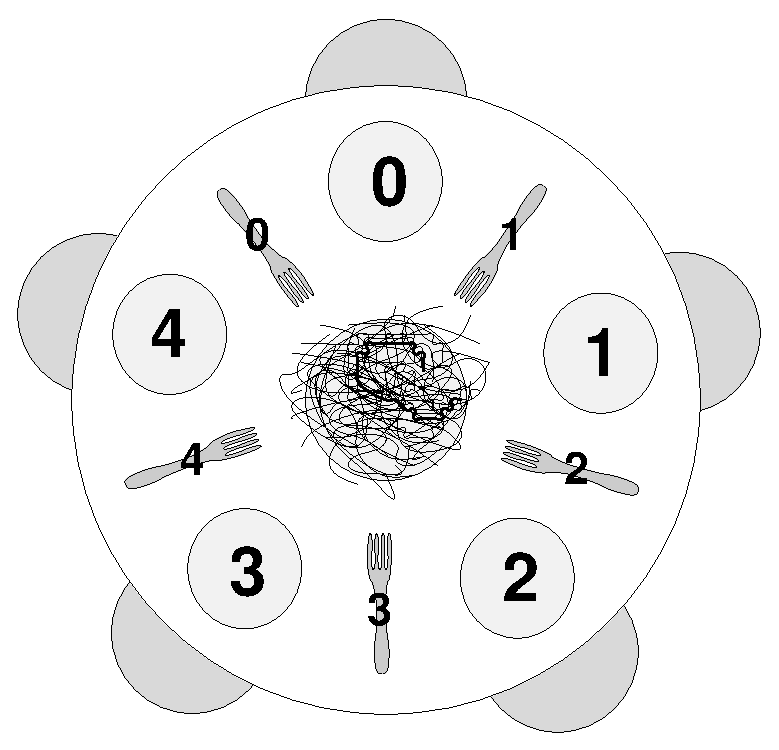
\includegraphics[height=2in]{table.eps}}

Assuming that the philosophers know how to {\tt think} and {\tt eat},
our job is to write a version of {\tt get\_forks} and {\tt put\_forks}
that satisfies the following constraints:

\begin{itemize}

\item Only one philosopher can hold a fork at a time.

\item It must be impossible for a deadlock to occur.

\item It must be impossible for a philosopher to starve waiting
for a fork.

\item It must be possible for more than one philosopher
to eat at the same time.

\end{itemize}

The last requirement is one way of saying that the solution
should be efficient; that is, it should allow the maximum amount
of concurrency.

We make no assumption about how long {\tt eat} and {\tt think} take,
except that {\tt eat} has to terminate eventually.  Otherwise, the
third constraint is impossible---if a philosopher keeps one of the
forks forever, nothing can prevent the neighbors from starving.

To make it easy for philosophers to refer to their forks,
we can use the functions {\tt left} and {\tt right}:

\begin{lstlisting}[title={Which fork?}]{}
def left(i): return i
def right(i): return (i + 1) % 5
\end{lstlisting}

The {\tt \%} operator wraps around when it gets to 5, so
{\tt (4 + 1) \% 5 = 0}.

Since we have to enforce exclusive access to the forks,
it is natural to use a list of Semaphores, one for
each fork.  Initially, all the forks are available.

\begin{lstlisting}[title={Variables for dining philosophers}]{}
forks = [Semaphore(1) for i in range(5)]
\end{lstlisting}

This notation for initializing a list might be unfamiliar to
readers who don't use Python.  The {\tt range} function returns
a list with 5 elements; for each element of this list, Python
creates a Semaphore with initial value 1 and assembles the
result in a list named {\tt forks}.

Here is an initial attempt at {\tt get\_fork} and {\tt put\_fork}:

\begin{lstlisting}[title={Dining philosophers non-solution}]{}
def get_forks(i):
    fork[right(i)].wait()
    fork[left(i)].wait()

def put_forks(i):
    fork[right(i)].signal()
    fork[left(i)].signal()
\end{lstlisting}

It's clear that this solution satisfies the first constraint, but
we can be pretty sure it doesn't satisfy the other two, because
if it did, this wouldn't be an interesting problem and you would
be reading Chapter~\ref{next}.

Puzzle: what's wrong?


\clearemptydoublepage
\subsection{Deadlock \#5}

The problem is that the table is round.  As a result, each philosopher
can pick up a fork and then wait forever for the other fork.  Deadlock!

Puzzle: write a solution to this problem that prevents deadlock.

Hint: one way to avoid deadlock is to think about the conditions
that make deadlock possible and then change one of those conditions.
In this case, the deadlock is fairly fragile---a very small change
breaks it.

\clearemptydoublepage
\subsection{Dining philosophers hint \#1}

If only four philosophers are allowed at the table at a time,
deadlock is impossible.

First, convince yourself that this claim is true, then write code that
limits the number of philosophers at the table.


\clearemptydoublepage
\subsection{Dining philosophers solution \#1}

If there are only four philosophers at the table, then in the
worst case each one picks up a fork.  Even then, there is a fork
left on the table, and that fork has two neighbors, each of
which is holding another fork.  Therefore, either of these
neighbors can pick up the remaining fork and eat.

We can control the number of philosophers at the table with
a Multiplex named {\tt footman} that is initialized to 4.
Then the solution looks like this:

\begin{lstlisting}[title={Dining philosophers solution \#1}]{}
def get_forks(i):
    footman.wait()
    fork[right(i)].wait()
    fork[left(i)].wait()

def put_forks(i):
    fork[right(i)].signal()
    fork[left(i)].signal()
    footman.signal()
\end{lstlisting}

In addition to avoiding deadlock, this solution also guarantees that
no philosopher starves.
Imagine that you
are sitting at the table and both of your neighbors are eating.  You
are blocked waiting for your right fork.  Eventually your right
neighbor will put it down, because {\tt eat} can't run forever.  Since
you are the only thread waiting for that fork, you will necessarily
get it next.  By a similar argument, you cannot starve waiting for
your left fork.

Therefore, the time a philosopher can spend at the table is bounded.
That implies that the wait time to get into the room is also bounded,
as long as {\tt footman} has Property 4 (see Section ~\ref{props}).

This solution shows that
by controlling the number of philosophers, we can avoid deadlock.
Another way to avoid deadlock is to change the order in which the
philosophers pick up forks.  In the original non-solution, the
philosophers are ``righties''; that is, they pick up the right fork
first.  But what happens if Philosopher 0 is a leftie?

Puzzle: prove that if there is at least one leftie and at least one
rightie, then deadlock is not possible.

Hint: deadlock can only occur when all 5 philosophers are holding
one fork and waiting, forever, for the other.  Otherwise, one of
them could get both forks, eat, and leave.

The proof works by contradiction.  First, assume that deadlock is
possible.  Then choose one of the supposedly deadlocked philosophers.
If she's a leftie, you can prove that the philosophers are all
lefties, which is a contradiction.  Similarly, if she's a rightie, you
can prove that they are all righties.  Either way you get a
contradiction; therefore, deadlock is not possible.


\clearemptydoublepage
\subsection{Dining philosopher's solution \#2}

In the asymmetric solution to the Dining philosophers problem,
there has to be at least one leftie and at least one rightie at
the table.  In that case, deadlock is impossible.  The previous
hint outlines the proof.  Here are the details.

Again, if deadlock is possible, it occurs when all 5 philosophers
are holding one fork and waiting for the other.  If we assume that
Philosopher $j$ is a leftie, then she must be holding her left
fork and waiting for her right.  Therefore her neighbor to the right,
Philosopher $k$, must be holding his left fork and waiting for
his right neighbor; in other words, Philosopher $k$ must be a leftie.
Repeating the same argument, we can prove that the philosophers
are all lefties, which contradicts the original claim that there
is at least one rightie.  Therefore deadlock is not possible.

The same argument we used for the previous solution also proves
that starvation is impossible for this solution.


\clearemptydoublepage
\subsection{Tanenbaum's solution}

There is nothing wrong with the previous solutions, but just for
completeness, let's look at some alternatives.  One of the best known
is the one that appears in Tanenbaum's popular operating systems
textbook \cite{tanenbaum}.
For each philosopher there is a state variable that
indicates whether the philosopher is thinking, eating, or waiting to
eat (``hungry'') and a semaphore that indicates whether the
philosopher can start eating.  Here are the variables:

\begin{lstlisting}[title={Variables for Tanenbaum's solution}]{}
state = ['thinking'] * 5
sem = [Semaphore(0) for i in range(5)]
mutex = Semaphore(1)
\end{lstlisting}

The initial value of {\tt state} is a list of 5 copies of {\tt
'thinking'}.  {\tt sem} is a list of 5 semaphores with the initial
value 0.  Here is the code:

\begin{lstlisting}[title={Tanenbaum's solution}]{}
def get_fork(i):
    mutex.wait()
    state[i] = 'hungry'
    test(i)
    mutex.signal()
    sem[i].wait()

def put_fork(i):
    mutex.wait()
    state[i] = 'thinking'
    test(right(i))
    test(left(i))
    mutex.signal()

def test(i):
    if state[i] == 'hungry' and
    state[left (i)]  != 'eating' and
    state[right (i)] != 'eating':
        state[i] = 'eating'
        sem[i].signal()
\end{lstlisting}

% NOTE: need to fix this; see email from David Furcy.

The {\tt test} function checks whether the $i$th philosopher can
start eating, which he can if he is hungry and
neither of his neighbors are eating.  If so, the {\tt test} signals
semaphore $i$.

There are two ways a philosopher gets to eat.  In the first case, the
philosopher executes {\tt get\_forks}, finds the forks available, and
proceeds immediately.  In the second case, one of the neighbors is
eating and the philosopher blocks on its own semaphore.  Eventually,
one of the neighbors will finish, at which point it executes {\tt
test} on both of its neighbors.  It is possible that both tests
will succeed, in which case the neighbors can run concurrently.
The order of the two tests doesn't matter.

In order to access {\tt state} or invoke {\tt test}, a thread
has to hold {\tt mutex}.  Thus, the operation of checking and
updating the array is atomic.  Since a philosopher can only proceed
when we know both forks are available, exclusive access to the forks
is guaranteed.

No deadlock is possible, because the only semaphore that is accessed
by more than one philosopher is {\tt mutex}, and no thread executes
{\tt wait} while holding {\tt mutex}.

But again, starvation is tricky.

Puzzle: Either convince yourself that Tanenbaum's solution prevents
starvation or find a repeating pattern that allows a thread to starve
while other threads make progress.


\clearemptydoublepage
\subsection{Starving Tanenbaums}

Unfortunately, this solution is not starvation-free.  Gingras
demonstrated that there are repeating patterns that allow a
thread to wait forever while other threads come and go
\cite{gingras90dining}.

Imagine that we are trying to starve Philosopher 0.  Initially,
2 and 4 are at the table and 1 and 3 are hungry.  Imagine that 2 gets up and
1 sit downs; then 4 gets up and 3 sits down.
Now we are in the mirror image of the starting position.

If 3 gets up and 4 sits
down, and then 1 gets up and 2 sits down, we are back
where we started.  We could repeat the cycle indefinitely and
Philosopher 0 would starve.

So, Tanenbaum's solution doesn't satisfy all the requirements.




\clearemptydoublepage
\section {Cigarette smokers problem}

The cigarette smokers problem problem was originally presented by
Suhas Patil \cite{patil}, who claimed that it cannot be solved with
semaphores.  That claim comes with some qualifications, but in
any case the problem is interesting and challenging.

Four threads are involved: an agent and three smokers.  The smokers
loop forever, first waiting for ingredients, then making and smoking
cigarettes.  The ingredients are tobacco, paper, and matches.

We assume that the agent has an infinite supply of all three
ingredients, and each smoker has an infinite supply of one of
the ingredients; that is, one smoker has matches, another has
paper, and the third has tobacco.

The agent repeatedly chooses two different ingredients at random
and makes them available to the smokers.  Depending on which
ingredients are chosen, the smoker with the complementary ingredient
should pick up both resources and proceed.

For example, if the agent puts out tobacco and paper, the
smoker with the matches should pick up both ingredients, make
a cigarette, and then signal the agent.

To explain the premise, the agent represents an operating system that
allocates resources, and the smokers represent applications that need
resources.  The problem is to make sure that if resources are
available that would allow one more applications to proceed,
those applications should be woken up.  Conversely, we want to avoid
waking an application if it cannot proceed.



Based on this premise, there are three versions of this problem
that often appear in textbooks:

\begin{description}

\item[The impossible version:] Patil's version imposes restrictions on
the solution.  First, you are not allowed to modify the agent code.
If the agent represents an operating system, it makes sense to assume
that you don't want to modify it every time a new application comes
along.  The second restriction is that you can't use conditional
statements or an array of semaphores.  With these constraints, the
problem cannot be solved, but as Parnas points out, the second
restriction is pretty artificial \cite{Parnas}.  With constraints like
these, a lot of problems become unsolvable.

\item[The interesting version:] This version keeps the first
restriction---you can't change the agent code---but it drops the others.

\item[The trivial version:] In some textbooks, the problem specifies
that the agent should signal the smoker that should go next, according
to the ingredients that are available.  This version of the problem
is uninteresting because it makes the whole premise, the ingredients
and the cigarettes, irrelevant.  Also, as a practical matter, it is
probably not a good idea to require the agent to know about the other
threads and what they are waiting for.  Finally, this version of
the problem is just too easy.

\end{description}

Naturally, we will focus on the interesting version.  To complete
the statement of the problem, we need to specify the agent code.
The agent uses the following semaphores:

\begin{lstlisting}[title={Agent semaphores}]{}
agentSem = Semaphore(1)
tobacco = Semaphore(0)
paper = Semaphore(0)
match = Semaphore(0)
\end{lstlisting}

The agent is actually made up of three concurrent
threads, Agent A, Agent B and Agent C.  Each waits on
{\tt agentSem}; each time {\tt agentSem} is signaled,
one of the Agents wakes up and provides ingredients by
signaling two semaphores.

\begin{lstlisting}[title={Agent A code}]{}
agentSem.wait()
tobacco.signal()
paper.signal()
\end{lstlisting}

\begin{lstlisting}[title={Agent B code}]{}
agentSem.wait()
paper.signal()
match.signal()
\end{lstlisting}

\begin{lstlisting}[title={Agent C code}]{}
agentSem.wait()
tobacco.signal()
match.signal()
\end{lstlisting}

This problem is hard because the natural solution does not
work.  It is tempting to write something like:

\begin{lstlisting}[title={Smoker with matches}]{}
tobacco.wait()
paper.wait()
agentSem.signal()
\end{lstlisting}

\begin{lstlisting}[title={Smoker with tobacco}]{}
paper.wait()
match.wait()
agentSem.signal()
\end{lstlisting}

\begin{lstlisting}[title={Smoker with paper}]{}
tobacco.wait()
match.wait()
agentSem.signal()
\end{lstlisting}

What's wrong with this solution?

\clearemptydoublepage
\subsection{Deadlock \#6}

The problem with the previous solution is the possibility
of deadlock.  Imagine that the agent puts out tobacco and
paper.  Since the smoker with matches is waiting on {\tt tobacco},
it might be unblocked.  But the smoker with tobacco is
waiting on {\tt paper}, so it is possible (even likely) that
it will also be unblocked.  Then the first thread will block
on {\tt paper} and the second will block on {\tt match}.
Deadlock!

\clearemptydoublepage
\subsection{Smokers problem hint}

The solution proposed by Parnas uses three helper threads
called ``pushers'' that respond to the signals from the agent,
keep track of the available ingredients, and signal the
appropriate smoker.

The additional variables and semaphores are

\begin{lstlisting}[title={Smokers problem hint}]{}
isTobacco = isPaper = isMatch = False
tobaccoSem = Semaphore(0)
paperSem = Semaphore(0)
matchSem = Semaphore(0)
\end{lstlisting}

The boolean variables indicate whether or not an ingredient
is on the table.  The pushers use {\tt tobaccoSem} to signal
the smoker with tobacco, and the other semaphores likewise.


\clearemptydoublepage
\subsection{Smoker problem solution}

Here is the code for one of the pushers:

\begin{lstlisting}[title={Pusher A}]{}
tobacco.wait()
mutex.wait()
    if isPaper:
        isPaper = False
        matchSem.signal()
    elif isMatch:
        isMatch = False
        paperSem.signal()
    else: 
        isTobacco = True
mutex.signal()
\end{lstlisting}

This pusher wakes up any time there is tobacco on the
table.  If it finds {\tt isPaper} true, it knows that
Pusher B has already run, so it can signal the smoker
with matches.  Similarly, if it finds a match on the
table, it can signal the smoker with paper.

But if Pusher A runs first, then it will find both
{\tt isPaper} and {\tt isMatch} false.  It cannot signal
any of the smokers, so it sets {\tt isTobacco}.

The other pushers are similar.  Since the pushers do all
the real work, the smoker code is trivial:

\begin{lstlisting}[title={Smoker with tobacco}]{}
tobaccoSem.wait()
makeCigarette()
agentSem.signal()
smoke()
\end{lstlisting}

Parnas presents a similar solution that assembles the
boolean variables, bitwise, into an integer, and then
uses the integer as an index into an array of semaphores.
That way he can avoid using conditionals (one of the
artificial constraints).  The resulting code is a bit
more concise, but its function is not as obvious.


\subsection{Generalized Smokers Problem}

Parnas suggested that the smokers problem becomes more
difficult if we modify the agent, eliminating the requirement
that the agent wait after putting out ingredients.  In this
case, there might be multiple instances of an ingredient on
the table.

Puzzle: modify the previous solution to deal with this
variation.

\clearemptydoublepage
\subsection{Generalized Smokers Problem Hint}

If the agents don't wait for the smokers, ingredients might
accumulate on the table.  Instead of using boolean values to
keep track of ingredients, we need integers to count them.

\begin{lstlisting}[title={Generalized Smokers problem hint}]{}
numTobacco = numPaper = numMatch = 0
\end{lstlisting}


\clearemptydoublepage
\subsection{Generalized Smokers Problem Solution}
\label{smoker}

Here is the modified code for Pusher A:

\begin{lstlisting}[title={Pusher A}]{}
tobacco.wait()
mutex.wait()
    if numPaper:
        numPaper -= 1
        matchSem.signal()
    elif numMatch:
        numMatch -= 1
        paperSem.signal()
    else: 
        numTobacco += 1
mutex.signal()
\end{lstlisting}

One way to visualize this problem is to imagine that when an
Agent runs, it creates two pushers, gives each of them one ingredient,
and puts them in a room with all the other pushers.  Because of the
mutex, the pushers file into a room where there are
three sleeping smokers and a table.  One at a time, each pusher enters
the room and checks the ingredients on the table.  If he can
assemble a complete set of ingredients, he takes them off the table
and wakes the corresponding smoker.  If not, he leaves his ingredient
on the table and leaves without waking anyone.

This is an example of a pattern we will see several times, which
I call a {\bf scoreboard}.  The variables {\tt numPaper}, {\tt numTobacco}
and {\tt numMatch} keep track of the state of the system.  As each
thread files through the mutex, it checks the state as if looking
at the scoreboard, and reacts accordingly.


\clearemptydoublepage
\chapter{Less classical synchronization problems}
\label{next}


\section{The dining savages problem}

This problem is from Andrews's 
{\em Concurrent Programming} \cite{andrews}.

\begin {quotation}
A tribe of savages eats communal dinners from a large pot that can
hold M servings of stewed missionary\footnote{This problem is based on
a cartoonish representation of the history of Western missionaries
among hunter-gatherer societies.  Some humor is intended by the
allusion to the Dining Philosophers problem, but the representation of
``savages'' here isn't intended to be any more realistic than the
previous representation of philosophers.  If you are interested in
hunter-gatherer societies, I recommend Jared Diamond's {\em Guns,
Germs and Steel}, Napoleon Chagnon's {\em The Yanomamo}, and Redmond
O'Hanlon's {\em In Trouble Again}, but not Tierney's {\em Darkness in
El Dorado}, which I believe is unreliable.}.  When a savage wants to
eat, he helps himself from the pot, unless it is empty.  If the pot is
empty, the savage wakes up the cook and then waits until the cook has
refilled the pot.
\end{quotation}

Any number of savage threads run the following code:

\begin{lstlisting}[title={Unsynchronized savage code}]{}
while True:
    getServingFromPot()
    eat()
\end{lstlisting}

And one cook thread runs this code:

\begin{lstlisting}[title={Unsynchronized cook code}]{}
while True:
    putServingsInPot(M)
\end{lstlisting}

The synchronization constraints are:

\begin{itemize}

\item Savages cannot invoke {\tt getServingFromPot} if the
pot is empty.

\item The cook can invoke {\tt putServingsInPot} only if
the pot is empty.

\end{itemize}

Puzzle: Add code for the savages and the cook that
satisfies the synchronization constraints.


\clearemptydoublepage
\subsection{Dining Savages hint}

It is tempting to use a semaphore to keep track of the number of
servings, as in the producer-consumer problem.  But in order to signal
the cook when the pot is empty, a thread would have to know before
decrementing the semaphore whether it would have to wait, and we just
can't do that.

An alternative is to use a scoreboard to
keep track of the number of servings.  If a savage finds
the counter at zero, he wakes the cook and waits for a signal
that the pot is full.  Here are the variables I used:

\begin{lstlisting}[title={Dining Savages hint}]{}
servings = 0
mutex = Semaphore(1)
emptyPot = Semaphore(0)
fullPot = Semaphore(0)
\end{lstlisting}

Not surprisingly, {\tt emptyPot} indicates that the pot is empty and
{\tt fullPot} indicates that the pot is full.

\clearemptydoublepage
\subsection{Dining Savages solution}

My solution is a combination of the scoreboard pattern
with a rendezvous.
Here is the code for the cook:

\begin{lstlisting}[title={Dining Savages solution (cook)}]{}
while True:
    emptyPot.wait()
    putServingsInPot(M)
    fullPot.signal()
\end{lstlisting}

The code for the savages is only a little more complicated.
As each savage passes through the mutex, he checks the pot.
If it is empty, he signals the cook and waits.  Otherwise,
he decrements {\tt servings} and gets a serving from the pot.

\begin{lstlisting}[title={Dining Savages solution (savage)}]{}
while True:
    mutex.wait()
        if servings == 0:
            emptyPot.signal()
            fullPot.wait()
            servings = M
        servings -= 1
	getServingFromPot()
    mutex.signal()

    eat()
\end{lstlisting}

It might seem odd that the savage, rather than the cook, sets
{\tt servings = M}.  That's not really necessary; when the cook
runs {\tt putServingsInPot}, we know that the savage that holds
the mutex is waiting on {\tt fullPot}.  So the cook could
access {\tt servings} safely.  But in this case, I decided to
let the savage do it so that it is clear from looking at the
code that all accesses to {\tt servings} are inside the mutex.

This solution is deadlock-free.  The only opportunity for
deadlock comes when the savage that holds {\tt mutex} waits
for {\tt fullPot}.  While he is waiting, other savages are
queued on {\tt mutex}.  But eventually the cook will run and
signal {\tt fullPot}, which allows the waiting savage
to resume and release the mutex.

Does this solution assume that the pot is thread-safe, or does it
guarantee that {\tt putServingsInPot} and {\tt getServingFromPot}
are executed exclusively?


\clearemptydoublepage
\section{The barbershop problem}

The original barbershop problem was proposed by
Dijkstra.  A variation of it appears in 
Silberschatz and Galvin's {\em Operating Systems Concepts}
\cite{silberschatz}.

\begin {quotation}
A barbershop consists of a waiting room with $n$ chairs, and the
barber room containing the barber chair.  If there are no customers to
be served, the barber goes to sleep.  If a customer enters the
barbershop and all chairs are occupied, then the customer leaves the
shop.  If the barber is busy, but chairs are available, then the
customer sits in one of the free chairs.  If the barber is asleep, the
customer wakes up the barber.  Write a program to coordinate the
barber and the customers.
\end{quotation}

To make the problem a little more concrete, I added the
following information:

\begin{itemize}

\item Customer threads should invoke a function named {\tt getHairCut}.

\item If a customer thread arrives when the shop is full, 
it can invoke {\tt balk}, which does not return.

\item Barber threads should invoke {\tt cutHair}.

\item When the barber invokes {\tt cutHair} there should
be exactly one thread invoking {\tt getHairCut} concurrently.

\end{itemize}


\clearemptydoublepage
\subsection{Barbershop hint}

\begin{lstlisting}[title={Barbershop hint}]{}
customers = 0
mutex = Semaphore(1)
customer = Semaphore(0)
barber = Semaphore(0)
customerDone = Semaphore(0)
barberDone = Semaphore(0)
\end{lstlisting}

{\tt customers} counts the number of customers in the shop;
it is protected by {\tt mutex}.

The barber waits on {\tt customer} until a customer enters the
shop, then the customer waits on {\tt barber} until the barber
signals him to take a seat.

After the haircut, the customer signals {\tt customerDone} and
waits on {\tt barberDone}.

\clearemptydoublepage
\subsection{Barbershop solution}

This solution combines a scoreboard and two rendezvouses\footnote{The
  plural of rendezvous is rare, and not all dictionaries agree about
  what it is.  Another possibility is that the plural is also spelled
  ``rendezvous,'' but the final ``s'' is pronounced.}.  Here is the
code for customers:

\begin{lstlisting}[title={Barbershop solution (customer)}]{}
mutex.wait()
    if customers == n+1:
        mutex.signal()
        balk()
    customers += 1
mutex.signal()

customer.signal()
barber.wait()        

getHairCut()

customerDone.signal()
barberDone.wait()        

mutex.wait()
    customers -= 1
mutex.signal()
\end{lstlisting}

If there are $n$ customers in the waiting room and one in the
barber chair, then the shop is full and any customers that
arrive immediately invoke {\tt balk}.
Otherwise each customer signals {\tt customer} and waits on
{\tt barber}.

Here is the code for barbers:

\begin{lstlisting}[title={Barbershop solution (barber)}]{}
customer.wait()
barber.signal()

cutHair()

customerDone.wait()
barberDone.signal()
\end{lstlisting}

Each time a customer signals,
the barber wakes, signals {\tt barber}, and gives one
hair cut.  If another customer arrives while the barber
is busy, then on the next iteration the barber will pass
the {\tt customer} semaphore without sleeping.

The names for {\tt customer} and {\tt barber} are based on
the naming convention for a rendezvous, so {\tt customer.wait()}
means ``wait for a customer,'' not ``customers wait here.''


\clearemptydoublepage
\section {Hilzer's Barbershop problem}

William Stallings \cite{stallings} presents a more complicated version
of the barbershop problem, which he attributes to Ralph Hilzer at the
California State University at Chico.

\begin{quotation}
Our barbershop has three chairs, three barbers, and a waiting
area that can accommodate four customers on a sofa and that has
standing room for additional customers.  Fire codes limit the
total number of customers in the shop to 20.

A customer will not enter the shop if it is filled to capacity with
other customers.  Once inside, the customer takes a seat on the sofa
or stands if the sofa is filled.  When a barber is free, the customer
that has been on the sofa the longest is served and, if there are any
standing customers, the one that has been in the shop the longest
takes a seat on the sofa.  When a customer's haircut is finished, any
barber can accept payment, but because there is only one cash
register, payment is accepted for one customer at a time.  The barbers
divide their time among cutting hair, accepting payment, and sleeping
in their chair waiting for a customer.
\end{quotation}


In other words, the
following synchronization constraints apply:

\begin{itemize}

\item Customers invoke the following functions in order:
{\tt enterShop}, {\tt sitOnSofa},
{\tt sitInBarberChair}, {\tt pay},
{\tt exitShop}.

\item Barbers invoke {\tt cutHair} and {\tt acceptPayment}.

\item Customers cannot invoke {\tt enterShop} if the shop
is at capacity.

\item If the sofa is full, an arriving customer cannot invoke 
{\tt sitOnSofa} until one of the customers on the sofa invokes {\tt
sitInBarberChair}.

\item If all three barber chairs are busy, an arriving customer
cannot invoke {\tt sitInBarberChair} until one of the customers in a
chair invokes {\tt pay}.

\item The customer has to {\tt pay} before the barber can
{\tt acceptPayment}.

\item The barber must {\tt acceptPayment} before the customer can
{\tt exitShop}.

\end{itemize}

One difficulty with this problem is that in each waiting area (the
sofa and the standing room), customers have to be served in
first-in-first-out (FIFO) order.  If our implementation of semaphores
happens to enforce FIFO queueing, then we can use nested multiplexes
to create the waiting areas.  Otherwise we can use Fifo objects
as defined in Section~\ref{Fifo}.

Puzzle: Write code that enforces the synchronization
constraints for Hilzer's barbershop.


\subsection {Hilzer's barbershop hint}

Here are the variables I used in my solution:

\begin{lstlisting}[title={Hilzer's barbershop hint}]{}
customers = 0
mutex = Semaphore(1)
standingRoom = Fifo()
sofa = Fifo()
chair = Semaphore(3)
barber = Semaphore(0)
customer = Semaphore(0)
cash = Semaphore(0)
receipt = Semaphore(0)
\end{lstlisting}

{\tt mutex} protects {\tt customers}, which keeps track of the
number of customers in the shop so that if a thread arrives
when the shop is full, it can exit.  {\tt standingRoom} and
{\tt sofa} are Fifos that represent the waiting areas.  {\tt chair}
is a multiplex that limits the number of customers in the
seating area.

The other semaphores are used for the rendezvous between the
barber and the customers.  The customer signals {\tt barber} and
then wait on {\tt customer}.  Then the customer signals {\tt cash}
and waits on {\tt receipt}.

\clearemptydoublepage
\subsection {Hilzer's barbershop solution}

There is nothing new here; it's a combination of
patterns we've seen before.

\begin{lstlisting}[title={Hilzer's barbershop solution (customer)}]{}
mutex.wait()
    if customers == 20:
        mutex.signal()
        exitShop()
    customers += 1
mutex.signal()

standingRoom.wait()
enterShop()

sofa.wait()
sitOnSofa()
standingRoom.signal()

chair.wait()
sitInBarberChair()
sofa.signal()

customer.signal()
barber.wait()
getHairCut()

pay()
cash.signal()
receipt.wait()

mutex.wait()
    customers -= 1
mutex.signal()

exitShop()
\end{lstlisting}

The mechanism that counts the number of customers and allows
threads to exit is the same as in the previous problem.

In order to maintain FIFO order for the whole system, threads cascade
from {\tt standingRoom} to {\tt sofa} to {\tt chair}; as each thread
moves to the next stage, it signals the previous stage.

The exchange with the barber is basically two consecutive
rendezvouses.

The code for the barber is self-explanatory:


\begin{lstlisting}[title={Hilzer's barbershop solution (barber)}]{}
customer.wait()
barber.signal()
cutHair()

cash.wait()
acceptPayment()
receipt.signal()
\end{lstlisting}

If two customers signal {\tt cash} concurrently, there is no
way to know which waiting barber will get which signal, but the
problem specification says that's ok.  Any barber can take
money from any customer.

\clearemptydoublepage
\section{The Santa Claus problem}

This problem is from William Stallings's
{\em Operating Systems} \cite{stallings},
but he attributes it to John Trono of St. Michael's College in
Vermont.

\begin{quotation}
Stand Claus sleeps in his shop at the North Pole and can only be
awakened by either (1) all nine reindeer being back from their
vacation in the South Pacific, or (2) some of the elves having
difficulty making toys; to allow Santa to get some sleep, the elves
can only wake him when three of them have problems.  When three elves
are having their problems solved, any other elves wishing to visit
Santa must wait for those elves to return.  If Santa wakes up to find
three elves waiting at his shop's door, along with the last reindeer
having come back from the tropics, Santa has decided that the elves can
wait until after Christmas, because it is more important to get his
sleigh ready.  (It is assumed that the reindeer do not want to leave
the tropics, and therefore they stay there until the last possible
moment.)  The last reindeer to arrive must get Santa while the others
wait in a warming hut before being harnessed to the sleigh.
\end{quotation}

Here are some addition specifications:

\begin {itemize}

\item After the ninth reindeer arrives, Santa must invoke 
{\tt prepareSleigh}, and then all nine reindeer must
invoke {\tt getHitched}.

\item After the third elf arrives, Santa must invoke {\tt helpElves}.
Concurrently, all three elves should invoke {\tt getHelp}.

\item All three elves must invoke {\tt getHelp} before any additional
elves enter (increment the elf counter).

\end {itemize}

Santa should run in a loop so he can help many sets of elves.
We can assume that there are exactly 9 reindeer, but there may
be any number of elves.  

\clearemptydoublepage
\subsection {Santa problem hint}

\begin{lstlisting}[title={Santa problem hint}]{}
elves = 0
reindeer = 0
santaSem = Semaphore(0)
reindeerSem = Semaphore(0)
elfTex = Semaphore(1)
mutex = Semaphore(1)
\end{lstlisting}

{\tt elves} and {\tt reindeer} are counters, both protected
by {\tt mutex}.  Elves and reindeer get {\tt mutex} to modify the
counters; Santa gets it to check them.

Santa waits on {\tt santaSem} until either an elf or a reindeer
signals him.

The reindeer wait on {\tt reindeerSem} until Santa signals them to
enter the paddock and get hitched.

The elves use {\tt elfTex} to prevent additional elves from
entering while three elves are being helped.


\clearemptydoublepage
\subsection {Santa problem solution}

Santa's code is pretty straightforward.  Remember that it
runs in a loop.

\begin{lstlisting}[title={Santa problem solution (Santa)}]{}
santaSem.wait()
mutex.wait()
    if reindeer >= 9:
        prepareSleigh()
	reindeerSem.signal(9)
        reindeer -= 9
    else if elves == 3:
        helpElves()
mutex.signal()
\end{lstlisting}

When Santa wakes up, he checks which of the two conditions
holds and either deals with the reindeer or the waiting elves.
If there are nine reindeer waiting,
Santa invokes {\tt prepareSleigh}, then signals {\tt reindeerSem}
nine times, allowing the reindeer to invoke {\tt getHitched}.
If there are elves waiting, Santa just
invokes {\tt helpElves}.  There is no need for the elves to wait
for Santa; once they signal {\tt santaSem}, they can
invoke {\tt getHelp} immediately.

Santa doesn't have to decrement
the {\tt elves} counter because the elves do it on their way
out.

Here is the code for reindeer:

\begin{lstlisting}[title={Santa problem solution (reindeer)}]{}
mutex.wait()
    reindeer += 1
    if reindeer == 9:
        santaSem.signal()
mutex.signal()

reindeerSem.wait()
getHitched()
\end{lstlisting}

The ninth reindeer signals Santa and then joins the other
reindeer waiting on {\tt reindeerSem}.  When Santa signals, the
reindeer all execute {\tt getHitched}.

The elf code is similar, except that when the third elf arrives
it has to bar subsequent arrivals until the first three have
executed {\tt getHelp}.

\newpage
\begin{lstlisting}[title={Santa problem solution (elves)}]{}
elfTex.wait()
mutex.wait()
    elves += 1
    if elves == 3:
        santaSem.signal()
    else
        elfTex.signal()
mutex.signal()

getHelp()

mutex.wait()
    elves -= 1
    if elves == 0:
       elfTex.signal()
mutex.signal()
\end{lstlisting}

The first two elves release {\tt elfTex} at the same time they release
the {\tt mutex}, but the last elf holds {\tt elfTex}, barring other
elves from entering until all three elves have invoked {\tt getHelp}.

The last elf to leave releases {\tt elfTex}, allowing the
next batch of elves to enter.

\newpage
\section{Building H$_2$O}
\label{water}

This problem has been a staple of the Operating Systems class
at U.C. Berkeley for at least a decade.  It seems to be based on
an exercise in Andrews's {\em Concurrent Programming} \cite{andrews}.

There are two kinds of threads, oxygen and hydrogen.  In order
to assemble these threads into water molecules, we have to
create a barrier that makes each thread wait until a
complete molecule is ready to proceed.

As each thread passes the barrier, it should invoke
{\tt bond}.  You must guarantee that all the threads
from one molecule invoke {\tt bond} before any of the threads
from the next molecule do.

In other words:

\begin{itemize}

\item If an oxygen thread arrives at the barrier when no
hydrogen threads are present, it has to wait for two
hydrogen threads.

\item If a hydrogen thread arrives at the barrier when
no other threads are present, it has to wait for an
oxygen thread and another hydrogen thread.

\end{itemize}

We don't have to worry about matching the threads up explicitly; that
is, the threads do not necessarily know which other threads they are
paired up with.  The key is just that threads pass the barrier in
complete sets; thus, if we examine the sequence of threads that invoke
{\tt bond} and divide them into groups of three, each group should
contain one oxygen and two hydrogen threads.

Puzzle: Write synchronization code for oxygen and hydrogen
molecules that enforces these constraints.


\clearemptydoublepage
\subsection {H$_2$O hint}

Here are the variables I used in my solution:

\begin{lstlisting}[title={Water building hint}]{}
mutex = Semaphore(1)
oxygen = 0
hydrogen = 0
barrier = Barrier(3)
oxyQueue = Semaphore(0)
hydroQueue = Semaphore(0)
\end{lstlisting}

{\tt oxygen} and {\tt hydrogen} are counters, protected by {\tt mutex}.
{\tt barrier} is where each set of three threads meets after
invoking {\tt bond} and before allowing the next set of threads
to proceed.

{\tt oxyQueue} is the semaphore oxygen threads wait on;
{\tt hydroQueue} is the semaphore hydrogen threads wait on.
I am using the naming convention for queues, so
{\tt oxyQueue.wait()} means ``join the oxygen queue'' and
{\tt oxyQueue.signal()} means ``release an oxygen thread from
the queue.''


\clearemptydoublepage
\subsection {H$_2$O solution}

Initially {\tt hydroQueue} and {\tt oxyQueue} are locked.  When
an oxygen thread arrives it signals {\tt hydroQueue} twice,
allowing two hydrogens to proceed.  Then the oxygen thread waits
for the hydrogen threads to arrive.

\begin{lstlisting}[title={Oxygen code}]{}
mutex.wait()
oxygen += 1
if hydrogen >= 2:
    hydroQueue.signal(2)
    hydrogen -= 2
    oxyQueue.signal()
    oxygen -= 1
else:
    mutex.signal()

oxyQueue.wait()
bond()

barrier.wait()
mutex.signal()
\end{lstlisting}

As each oxygen thread enters, it gets the mutex and checks the scoreboard.
If there are at least two hydrogen threads waiting, it signals two of
them and itself and then bonds.  If not, it releases the mutex and
waits.

After bonding, threads wait at the barrier until all three threads
have bonded, and then the oxygen thread releases the mutex.  Since
there is only one oxygen thread in each set of three, we are guaranteed
to signal {\tt mutex} once.

The code for hydrogen is similar:

\begin{lstlisting}[title={Hydrogen code}]{}
mutex.wait()
hydrogen += 1
if hydrogen >= 2 and oxygen >= 1:
    hydroQueue.signal(2)
    hydrogen -= 2
    oxyQueue.signal()
    oxygen -= 1
else:
    mutex.signal()

hydroQueue.wait()
bond()

barrier.wait()
\end{lstlisting}

An unusual feature of this solution is that
the exit point of the mutex is ambiguous.  In
some cases, threads enter the mutex, update the counter, and exit the
mutex.  But when a thread arrives that forms a complete set, it has to
keep the mutex in order to bar subsequent threads until the current
set have invoked {\tt bond}.

After invoking {\tt bond}, the three threads wait at a barrier.
When the barrier opens, we know that all three threads have invoked
{\tt bond} and that one of them holds the mutex.  We don't know
{\em which} thread holds the mutex, but it doesn't matter as long
as only one of them releases it.  Since we know there is only one
oxygen thread, we make it do the work.

This might seem wrong, because until now it
has generally been true that a thread has to hold a lock in
order to release it.  But there is no rule that says that has
to be true.  This is one of those cases where it can be misleading
to think of a mutex as a token that threads acquire and release.


\section {River crossing problem}

This is from a problem set written by Anthony Joseph
at U.C. Berkeley, but I don't know if he is the original author.
It is similar to the H$_2$O problem in the sense that it is
a peculiar sort of barrier that only allows threads to pass
in certain combinations.

Somewhere near Redmond, Washington there is a rowboat that is used by
both Linux hackers and Microsoft employees (serfs) to cross a river.  The
ferry can hold exactly four people; it won't leave the shore with more
or fewer.  To guarantee the safety of the passengers, it is not
permissible to put one hacker in the boat with three serfs, or to
put one serf with three hackers.  Any other combination is safe.

As each thread boards the boat it should invoke a function
called {\tt board}.  You must guarantee that all four threads
from each boatload invoke {\tt board} before any of the threads
from the next boatload do.

After all four threads have invoked {\tt board}, exactly one of
them should call a function named {\tt rowBoat}, indicating
that that thread will take the oars.  It doesn't matter which thread
calls the function, as long as one does.

Don't worry about the direction of travel.  Assume we are
only interested in traffic going in one of the directions.


\clearemptydoublepage
\subsection {River crossing hint}

Here are the variables I used in my solution:

\begin{lstlisting}[title={River crossing hint}]{}
barrier = Barrier(4)
mutex = Semaphore(1)
hackers = 0
serfs = 0
hackerQueue = Semaphore(0)
serfQueue = Semaphore(0)
local isCaptain = False
\end{lstlisting}

{\tt hackers} and {\tt serfs} count the number of hackers
and serfs waiting to board.  Since they are both protected by
{\tt mutex}, we can check the condition of both variables without
worrying about an untimely update.  This is another example
of a scoreboard.

{\tt hackerQueue} and {\tt serfQueue} allow us to control the number
of hackers and serfs that pass.  The barrier
makes sure that all four threads have invoked
{\tt board} before the captain invokes {\tt rowBoat}.

{\tt isCaptain} is a local variable that
indicates which thread should invoke {\tt row}.

\clearemptydoublepage
\subsection {River crossing solution}

The basic idea of this solution is that each arrival updates
one of the counters and then checks whether it makes a
full complement, either by being the fourth of its kind or
by completing a mixed pair of pairs.

I'll present the code for hackers; the serf code is
symmetric (except, of course, that it is 1000 times bigger,
full of bugs, and it contains an embedded web browser):

\begin{lstlisting}[title={River crossing solution}]{}
mutex.wait()
    hackers += 1
    if hackers == 4:
        hackerQueue.signal(4)                
	hackers = 0
	isCaptain = True
    elif hackers == 2 and serfs >= 2:
        hackerQueue.signal(2)                
        serfQueue.signal(2)                  
	serfs -= 2
	hackers = 0
	isCaptain = True
    else:
        mutex.signal()      # captain keeps the mutex

hackerQueue.wait()           

board()
barrier.wait()            

if isCaptain:
    rowBoat()
    mutex.signal()          # captain releases the mutex
\end{lstlisting}

As each thread files through the mutual exclusion section, it
checks whether a complete crew is ready to board.  If so, it
signals the appropriate threads, declares itself captain, and
holds the mutex in order to bar additional threads until the
boat has sailed.

The barrier keeps track of how many threads have boarded.
When the last thread arrives, all threads proceed.
The captain invoked {\tt row} and then (finally) releases the mutex.


\clearemptydoublepage
\section{The roller coaster problem}

This problem is from Andrews's {\em Concurrent
Programming} \cite{andrews}, but he attributes it to J. S. Herman's
Master's thesis.

\begin {quotation}
Suppose there are $n$ passenger threads and a car thread.  The passengers
repeatedly wait to take rides in the car, which can hold $C$ passengers,
where $C<n$.  The car can go around the tracks only when it is full.
\end{quotation}

Here are some additional details:

\begin{itemize}

\item Passengers should invoke {\tt board} and {\tt unboard}.

\item The car should invoke {\tt load}, {\tt run} and {\tt unload}.

\item Passengers cannot board until the car has invoked {\tt load}

\item The car cannot depart until $C$ passengers have boarded.

\item Passengers cannot unboard until the car
has invoked {\tt unload}.

\end{itemize}

Puzzle: Write code for the passengers and car that enforces these
constraints.


\clearemptydoublepage
\subsection{Roller Coaster hint}

\begin{lstlisting}[title={Roller Coaster hint}]{}
mutex = Semaphore(1)
mutex2 = Semaphore(1)
boarders = 0
unboarders = 0
boardQueue = Semaphore(0)
unboardQueue = Semaphore(0)
allAboard = Semaphore(0)
allAshore = Semaphore(0)
\end{lstlisting}

{\tt mutex} protects {\tt passengers}, which counts the number of
passengers that have invoked {\tt boardCar}.  

Passengers wait on {\tt boardQueue} before boarding and
{\tt unboardQueue} before unboarding.  {\tt allAboard}
indicates that the car is full.


\clearemptydoublepage
\subsection{Roller Coaster solution}

Here is my code for the car thread:

\begin{lstlisting}[title={Roller Coaster solution (car)}]{}
load()
boardQueue.signal(C)
allAboard.wait()

run()

unload()
unboardQueue.signal(C)
allAshore.wait()
\end{lstlisting}

When the car arrives, it signals $C$ passengers,
then waits for the last one to signal {\tt allAboard}.
After it departs, it allows $C$ passengers to disembark,
then waits for {\tt allAshore}.

\begin{lstlisting}[title={Roller Coaster solution (passenger)}]{}
boardQueue.wait()
board()

mutex.wait()
   boarders += 1
   if boarders == C:
       allAboard.signal()
       boarders = 0
mutex.signal()

unboardQueue.wait()
unboard()

mutex2.wait()
   unboarders += 1
   if unboarders == C:
       allAshore.signal()
       unboarders = 0
mutex2.signal()
\end{lstlisting}

Passengers wait for the car before boarding, naturally, and wait for
the car to stop before leaving.  The last passenger to board signals
the car and resets the passenger counter.


\clearemptydoublepage
\subsection{Multi-car Roller Coaster problem}

This solution does not generalize to the case where there is more
than one car.  In order to do that, we have to satisfy some additional
constraints:

\begin{itemize}

\item Only one car can be boarding at a time.

\item Multiple cars can be on the track concurrently.

\item Since cars can't pass each other, they have to unload
in the same order they boarded.

\item All the threads from one carload must disembark before
any of the threads from subsequent carloads.

\end{itemize}

Puzzle: modify
the previous solution to handle the additional constraints.
You can assume that there are $m$ cars, and that
each car has a local variable named {\tt i}
that contains an identifier between 0 and $m-1$.


\clearemptydoublepage
\subsection{Multi-car Roller Coaster hint}

I used two lists of semaphores to keep the cars in order.  One
represents the loading area and one represents the unloading area.
Each list contains one semaphore for each car.
At any time, only one semaphore in each
list is unlocked, so that enforces the order threads can
load and unload.
Initially, only the semaphores for Car 0 are unlocked.
As each car enters the
loading (or unloading) it waits on its own semaphore; as it leaves it
signals the next car in line.

\begin{lstlisting}[title={Multi-car Roller Coaster hint}]{}
loadingArea = [Semaphore(0) for i in range(m)]
loadingArea[1].signal()
unloadingArea = [Semaphore(0) for i in range(m)]
unloadingArea[1].signal()
\end{lstlisting}

The function {\tt next} computes the identifier of the next
car in the sequence (wrapping around from $m-1$ to 0):

\begin{lstlisting}[title={Implementation of {\tt next}}]{}
def next(i):
    return (i + 1) % m
\end{lstlisting}



\clearemptydoublepage
\subsection{Multi-car Roller Coaster solution}

Here is the modified code for the cars:

\begin{lstlisting}[title={Multi-car Roller Coaster solution (car)}]{}
loadingArea[i].wait()
load()
boardQueue.signal(C)
allAboard.wait()
loadingArea[next(i)].signal()

run()

unloadingArea[i].wait()
unload()
unboardQueue.signal(C)
allAshore.wait()
unloadingArea[next(i)].signal()
\end{lstlisting}

The code for the passengers is unchanged.


\clearemptydoublepage
\chapter{Not-so-classical problems}

\section{The search-insert-delete problem}

This one is from Andrews's {\em Concurrent Programming} \cite{andrews}.

\begin {quotation}
Three kinds of threads share access to a singly-linked list:
searchers, inserters and deleters.  Searchers merely examine the list;
hence they can execute concurrently with each other.  Inserters add
new items to the end of the list; insertions must be mutually
exclusive to preclude two inserters from inserting new items at about
the same time.  However, one insert can proceed in parallel with any
number of searches.  Finally, deleters remove items from anywhere in
the list.  At most one deleter process can access the list at a time,
and deletion must also be mutually exclusive with searches and
insertions.
\end{quotation}

Puzzle: write code for searchers, inserters and deleters that
enforces this kind of three-way categorical mutual exclusion.


\clearemptydoublepage
\subsection{Search-Insert-Delete hint}

\begin{lstlisting}[title={Search-Insert-Delete hint}]{}
insertMutex = Semaphore(1)
noSearcher = Semaphore(1)
noInserter = Semaphore(1)
searchSwitch = Lightswitch()
insertSwitch = Lightswitch()
\end{lstlisting}

{\tt insertMutex} ensures that only one inserter is in its critical
section at a time.  {\tt noSearcher} and {\tt noInserter} indicate
(surprise) that there are no searchers and no inserters in their
critical sections; a deleter needs to hold both of these to enter.

{\tt searchSwitch} and {\tt insertSwitch} are used by searchers and
inserters to exclude deleters.


\clearemptydoublepage
\subsection{Search-Insert-Delete solution}

Here is my solution:

\begin{lstlisting}[title={Search-Insert-Delete solution (searcher)}]{}
searchSwitch.wait(noSearcher)
# critical section
searchSwitch.signal(noSearcher)
\end{lstlisting}

The only thing a searcher needs to worry about is a deleter.
The first searcher in takes {\tt noSearcher}; the last one out
releases it.

\begin{lstlisting}[title={Search-Insert-Delete solution (inserter)}]{}
insertSwitch.wait(noInserter)
insertMutex.wait()
# critical section
insertMutex.signal()
insertSwitch.signal(noInserter)
\end{lstlisting}

Similarly, the first inserter takes {\tt noInserter} and the last one
out releases it.  Since searchers and inserters compete for different
semaphores, they can be in their critical section concurrently.
But {\tt insertMutex} ensures that only one inserter is in the room
at a time.

\begin{lstlisting}[title={Search-Insert-Delete solution (deleter)}]{}
noSearcher.wait()
noInserter.wait()
# critical section
noInserter.signal()
noSearcher.signal()

\end{lstlisting}

Since the deleter holds both {\tt noSearcher} and {\tt noInserter},
it is guaranteed exclusive access.  Of course, any time we see
a thread holding more than one semaphore, we need to check for
deadlocks.  By trying out a few scenarios, you should be able
to convince yourself that this solution is deadlock free.

On the other hand, like many categorical exclusion problems, this
one is prone to starvation.  As we saw in the Readers-Writers problem,
we can sometimes mitigate this problem by giving priority to one
category of threads according to application-specific criteria.
But in general it is difficult to write an efficient solution
(one that allows the maximum degree of concurrency)
that avoids starvation.



\section{The unisex bathroom problem}

I wrote this problem\footnote{Later I learned that a nearly
identical problem appears in Andrews's 
{\em Concurrent Programming}\cite{andrews}} when a friend of mine
left her position teaching physics at Colby College
and took a job at Xerox.

She was working in a cubicle in the basement of a
concrete monolith, and the nearest women's bathroom was two floors up.
She proposed to the Uberboss that they convert the men's bathroom
on her floor to a unisex bathroom, sort of like on Ally McBeal.

The Uberboss agreed, provided that the following synchronization
constraints can be maintained:

\begin {itemize}

\item There cannot be men and women in the bathroom
at the same time.

\item There should never be more than three
employees squandering company time in the bathroom.

\end{itemize}

Of course the solution should avoid deadlock.  For now, though, don't
worry about starvation.  You may assume that the bathroom is equipped
with all the semaphores you need.


\clearemptydoublepage
\subsection {Unisex bathroom hint}

Here are the variables I used in my solution:

\begin{lstlisting}[title={Unisex bathroom hint}]{}
empty = Semaphore(1)
maleSwitch = Lightswitch()
femaleSwitch = Lightswitch()
maleMultiplex = Semaphore(3)
femaleMultiplex = Semaphore(3)
\end{lstlisting}

{\tt empty} is 1 if the room is empty and 0 otherwise.

{\tt maleSwitch} allows men to bar women from the room.
When the first male enters, the lightswitch locks {\tt empty}, barring women;
When the last male exits, it unlocks {\tt empty}, allowing women
to enter.  Women do likewise using {\tt femaleSwitch}.

{\tt maleMultiplex} and {\tt femaleMultiplex} ensure that there are no
more than three men and three women in the system at a time.


\clearemptydoublepage
\subsection {Unisex bathroom solution}

Here is the female code:

\begin{lstlisting}[title={Unisex bathroom solution (female)}]{}
femaleSwitch.lock(empty)
    femaleMultiplex.wait()
        # bathroom code here
    femaleMultiplex.signal()
female Switch.unlock(empty)
\end{lstlisting}

The male code is similar.

Are there any problems with this solution?

\clearemptydoublepage
\subsection {No-starve unisex bathroom problem}

The problem with the previous solution is that it allows starvation.
A long line of women can arrive and enter while there is a man
waiting, and vice versa.

Puzzle: fix the problem.


\clearemptydoublepage
\subsection {No-starve unisex bathroom solution}

As we have seen before, we can use a turnstile to allow one
kind of thread to stop the flow of the other kind of thread.
This time we'll look at the male code:

\begin{lstlisting}[title={No-starve unisex bathroom solution (male)}]{}
turnstile.wait()
    maleSwitch.lock(empty)
turnstile.signal()

    maleMultiplex.wait()
        # bathroom code here
    maleMultiplex.signal()

maleSwitch.unlock (empty)
\end{lstlisting}

As long as there are men in the room, new arrivals will pass
through the turnstile and enter.  If there are women in the room
when a male arrives, the male will block inside the turnstile,
which will bar all later arrivals (male and female) from entering
until the current occupants leave.  At that point the male in
the turnstile enters, possibly allowing additional males to enter.

The female code is similar, so if there are men in the room an
arriving female will get stuck in the turnstile, barring additional
men.

This solution may not be efficient.  If
the system is busy, then there will often be several threads, male and
female, queued on the turnstile.  Each time {\tt empty} is signaled,
one thread will leave the turnstile and another will enter.  If the
new thread is the opposite gender, it will promptly block, barring
additional threads.  Thus, there will usually be only 1-2 threads in
the bathroom at a time, and the system will not take full advantage
of the available concurrency.


\section{Baboon crossing problem}

This problem is adapted from Tanenbaum's {\em Operating Systems:
Design and Implementation} \cite{tanenbaum}.
There is a deep canyon somewhere in
Kruger National Park, South Africa, and a single rope that spans the
canyon.  Baboons can cross the canyon by swinging hand-over-hand on
the rope, but if two baboons going in opposite directions meet in the
middle, they will fight and drop to their deaths.  Furthermore,
the rope is only strong enough to hold 5 baboons.  If there are
more baboons on the rope at the same time, it will break.

Assuming that we can teach the baboons to use semaphores, we
would like to design a synchronization scheme with the following
properties:

\begin{itemize}

\item Once a baboon has begun to cross, it is guaranteed
to get to the other side without running into a baboon going
the other way.

\item There are never more than 5 baboons on the rope.

\item A continuing stream of baboons crossing in one direction
should not bar baboons going the other way indefinitely
(no starvation).

\end{itemize}

I will not include a solution to this problem for reasons that
should be clear.


\section{The Modus Hall Problem}

This problem was written by Nathan Karst, one of the Olin students
living in Modus Hall\footnote{Modus Hall is one of several nicknames
for the modular buildings, aka Mods, that some students lived in while
the second residence hall was being built.} during the winter of 2005.

\begin{quote}
After a particularly heavy snowfall this winter, the denizens of Modus
Hall created a trench-like path between their cardboard shantytown and
the rest of campus.  Every day some of the residents walk to and from
class, food and civilization via the path; we will ignore the
indolent students who chose daily to drive to Tier 3.  We will also
ignore the direction in which pedestrians are traveling.  For some
unknown reason, students living in West Hall would occasionally find it
necessary to venture to the Mods.

Unfortunately, the path is not wide enough to allow two people
to walk side-by-side.  If two Mods persons meet at some point on the
path, one will gladly step aside into the neck high drift to accommodate
the other.  A similar situation will occur if two ResHall inhabitants
cross paths.  If a Mods heathen and a ResHall prude meet, however, a
violent skirmish will ensue with the victors determined solely by
strength of numbers; that is, the faction with the larger population will
force the other to wait.
\end{quote}

This is similar to the Baboon Crossing problem (in more ways than
one), with the added twist that control of the critical section is
determined by majority rule.  This has the potential to be an
efficient and starvation-free solution to the categorical exclusion
problem.

Starvation is avoided because while one faction controls the critical
section, members of the other faction accumulate in queue until they
achieve a majority.  Then they can bar new opponents from entering
while they wait for the critical section to clear.  I expect this
solution to be efficient because it will tend to move threads through
in batches, allowing maximum concurrency in the critical section.

Puzzle: write code that implements categorical exclusion with
majority rule.



\clearemptydoublepage
\subsection {Modus Hall problem hint}

Here are the variables I used in my solution.

\begin{lstlisting}[title={Modus problem hint}]{}
heathens = 0
prudes = 0
status = 'neutral'
mutex = Semaphore(1)
heathenTurn = Semaphore(1)
prudeTurn = Semaphore(1)
heathenQueue = Semaphore(0)
prudeQueue = Semaphore(0)
\end{lstlisting}

{\tt heathens} and {\tt prudes} are counters, and {\tt status} records
the status of the field, which can be `neutral', `heathens rule',
`prudes rule', `transition to heathens' or `transition to prudes'.
All three are protected by {\tt mutex} in the usual scoreboard
pattern.

{\tt heathenTurn} and {\tt prudeTurn} control access to the field
so that we can bar one side or the other during a transition.

{\tt heathenQueue} and {\tt prudeQueue} are where threads wait after
checking in and before taking the field.


\clearemptydoublepage
\subsection {Modus Hall problem solution}

Here is the code for heathens:

\begin{lstlisting}[title={Modus problem solution}]{}
heathenTurn.wait()
heathenTurn.signal()
(*\label{silentmajority}*)
mutex.wait()
heathens++

if status == 'neutral':
    status = 'heathens rule'
    mutex.signal()
elif status == 'prudes rule':
    if heathens > prudes:
        status = 'transition to heathens'
        prudeTurn.wait()
    mutex.signal()
    heathenQueue.wait()
elif status == 'transition to heathens':
    mutex.signal()
    heathenQueue.wait()
else
    mutex.signal()

# cross the field

mutex.wait()
heathens--

if heathens == 0:
    if status == 'transition to prudes':
        prudeTurn.signal()
    if prudes:
        prudeQueue.signal(prudes)
        status = 'prudes rule'
    else:
        status = 'neutral'
        
if status == 'heathens rule':
    if prudes > heathens:
        status = 'transition to prudes'
        heathenTurn.wait()

mutex.signal()
\end{lstlisting}

As each student checks in, he has to
consider the following cases:

\begin{itemize}

\item If the field is empty, the student lays claim for the heathens.

\item If the heathens currently in charge, but the new arrival
has tipped the balance, he locks the prude turnstile and the
system switches to transition mode.

\item If the prudes in charge, but the new arrival doesn't
tip the balance, he joins the queue.

\item If the system is transitioning to heathen control, the new arrival
joins the queue.

\item Otherwise we conclude that either the heathens are in charge, or the
system is transitioning to prude control.  In either case, this
thread can proceed.

\end{itemize}  

Similarly, as each student checks out, she has to consider several
cases.  

\begin{itemize}

\item If she is the last heathen to check out, she has to
consider the following:

    \begin{itemize}

    \item If the system is in transition, that means that the prude
      turnstile is locked, so she has to open it.

    \item If there are prudes waiting, she signals them and
      updates {\tt status} so the prudes are in charge.  If not, the
      new status is 'neutral'.

    \end{itemize}  

\item If she is not the last heathen to check out, she still has to
check the possibility that her departure will tip the balance.  In
that case, she closes the heathen turnstile and starts the
transition.

\end{itemize}

One potential difficulty of this solution is that any number
of threads could be interrupted at Line~\ref{silentmajority},
where they would have passed the turnstile but not yet checked in.
Until they check in, they are not counted, so the balance of
power may not reflect the number of threads that have passed the
turnstile.  Also, a transition ends when all the threads that have
checked in have also checked out.  At that point, there may
be threads (of both types) that have passed the turnstile.

These behaviors may affect efficiency---this solution does
not guarantee maximum concurrency---but they don't affect
correctness, if you accept that ``majority rule'' only applies
to threads that have registered to vote.


\clearemptydoublepage
\chapter{Not remotely classical problems}


% \clearemptydoublepage
\section{The sushi bar problem}

This problem was inspired by a problem proposed by Kenneth Reek \cite{reek}.
Imagine a sushi bar with 5 seats.  If you arrive while there is an
empty seat, you can take a seat immediately.  But if you arrive when
all 5 seats are full, that means that all of them are dining together,
and you will have to wait for the entire party to leave before you
sit down.

Puzzle: write code for customers entering and
leaving the sushi bar that enforces these requirements.

\clearemptydoublepage
\subsection {Sushi bar hint}

Here are the variables I used:

\begin{lstlisting}[title={Sushi bar hint}]{}
eating = waiting = 0
mutex = Semaphore(1)
block = Semaphore(0)
must_wait = False
\end{lstlisting}

{\tt eating} and {\tt waiting} keep track of the number of
threads sitting at the bar and waiting.  {\tt mutex} protects
both counters.  {\tt must\_wait} indicates that the bar is (or
has been) full, som incoming customers have to block
on {\tt block}.


\clearemptydoublepage
\subsection {Sushi bar non-solution}

Here is an incorrect solution Reek uses to illustrate one
of the difficulties of this problem.

\begin{lstlisting}[title={Sushi bar non-solution}]{}
mutex.wait()
if must_wait:
    waiting += 1
    mutex.signal()
    block.wait()

    mutex.wait()      # reacquire mutex (*\label{sushi1}*)
    waiting -= 1

eating += 1
must_wait = (eating == 5)
mutex.signal()

# eat sushi

mutex.wait()
eating -= 1
if eating == 0:
    n = min(5, waiting)
    block.signal(n)
    must_wait = False
mutex.signal()
\end{lstlisting}

Puzzle: what's wrong with this solution?


\clearemptydoublepage
\subsection {Sushi bar non-solution}

The problem is at Line~\ref{sushi1}.  If a customer arrives
while the bar is full, he has to give up the mutex while he
waits so that other customers can leave.  When the last customer
leaves, she signals {\tt block}, which wakes up at least some
of the waiting customers, and clears {\tt must\_wait}.

But when the customers wake up, they have to get the mutex
back, and that means they have to compete with incoming new
threads.  If new threads arrive and get the mutex first,
they could take all the seats before the waiting threads.
This is not just a question of injustice; it is possible for more
than 5 threads to be in the critical section concurrently, which
violates the synchronization constraints.

Reek provides two solutions to this problem, which appear
in the next two sections.

Puzzle: see if you can come up with two different correct solutions!

Hint: neither solution uses any additional variables.

\clearemptydoublepage
\subsection {Sushi bar solution \#1}

The only reason a waiting customer has to reacquire the mutex
is to update the state of {\tt eating} and {\tt waiting}, so
one way to solve the problem is to make the departing customer,
who already has the mutex, do the updating.

\begin{lstlisting}[title={Sushi bar solution \#1}]{}
mutex.wait()
if must_wait:
    waiting += 1
    mutex.signal()
    block.wait()
else:
    eating += 1
    must_wait = (eating == 5)
    mutex.signal()

# eat sushi

mutex.wait()
eating -= 1
if eating == 0:
    n = min(5, waiting)
    waiting -= n
    eating += n
    must_wait = (eating == 5)
    block.signal(n)
mutex.signal()
\end{lstlisting}

When the last departing customer releases the mutex, 
{\tt eating} has already been updated, so newly arriving customers
see the right state and block if necessary.  Reek calls this
pattern ``I'll do it for you,'' because the departing thread
is doing work that seems, logically, to belong to the waiting
threads.

A drawback of this approach is that is it a little more difficult
to confirm that the state is being updated correctly.


\clearemptydoublepage
\subsection {Sushi bar solution \#2}

Reek's alternative solution is based on the counterintuitive
notion that we can transfer a mutex from one thread to another!
In other words, one thread can acquire a lock and then another
thread can release it.  As long as both threads understand
that the lock has been transferred, there is nothing wrong with
this.

\begin{lstlisting}[title={Sushi bar solution \#2}]{}
mutex.wait()
if must_wait:
    waiting += 1
    mutex.signal()
    block.wait()     # when we resume, we have the mutex
    waiting -= 1

eating += 1
must_wait = (eating == 5)
if waiting and not must_wait:
    block.signal()            # and pass the mutex
else:
    mutex.signal()

# eat sushi

mutex.wait()
eating -= 1
if eating == 0: must_wait = False

if waiting and not must_wait:
    block.signal()            # and pass the mutex
else:
    mutex.signal()
\end{lstlisting}

If there are fewer than 5 customers at the bar and no one waiting, an
entering customer just increments {\tt eating} and releases the
mutex.  The fifth customer sets {\tt must\_wait}.

If {\tt must\_wait} is set, entering customers block until the last
customer at the bar clears {\tt must\_wait} and signals {\tt block}.
It is understood that the signaling thread gives up the mutex and the
waiting thread receives it.  Keep in mind, though, that this is an
invariant understood by the programmer, and documented in the
comments, but not enforced by the semantics of semaphores.  It is up
to us to get it right.

When the waiting thread resumes, we understand that it has
the mutex.  If there are other threads waiting,
it signals {\tt block} which, again,
passes the mutex to a waiting thread.  This process
continues, with each thread passing the mutex to the next until
there are no more chairs or no more waiting threads.  In either
case, the last thread releases the mutex and goes to sit down.

Reek calls this pattern ``Pass the baton,'' since the mutex
is being passed from one thread to the next like a baton in a
relay race.
One nice thing about this solution is that it is easy to confirm
that updates to {\tt eating} and {\tt waiting} are consistent.
A drawback is that it is harder to confirm that the mutex is
being used correctly.


% \clearemptydoublepage
\section{The child care problem}

Max Hailperin wrote this problem for his textbook {\em Operating
Systems and Middleware} \cite{hailperin}.  At a child care center,
state regulations require that there is always one adult present for
every three children.

Puzzle: Write code for child threads and adult threads that enforces
this constraint in a critical section.


\clearemptydoublepage
\subsection {Child care hint}

Hailperin suggests that you can {\em almost} solve this problem
with one semaphore.

\begin{lstlisting}[title={Child care hint}]{}
multiplex = Semaphore(0)
\end{lstlisting}

{\tt multiplex} counts the number of tokens available, where each token
allows a child thread to enter.  As adults enter, they signal {\tt
multiplex} three times; as they leave, they {\tt wait} three times.
But there is a problem with this solution.

Puzzle: what is the problem?


\clearemptydoublepage
\subsection {Child care non-solution}

Here is what the adult code looks like in Hailperin's non-solution:

\begin{lstlisting}[title={Child care non-solution (adult)}]{}
multiplex.signal(3)

# critical section

multiplex.wait()
multiplex.wait()
multiplex.wait()
\end{lstlisting}

The problem is a potential deadlock.  Imagine that there are
three children and two adults in the child care center.  The
value of {\tt multiplex} is 3, so either adult should be able
to leave.  But if both adults start to leave at the same time,
they might divide the available tokens between them, and both
block.

Puzzle: solve this problem with a minimal change.


\clearemptydoublepage
\subsection {Child care solution}

Adding a mutex solves the problem:

\begin{lstlisting}[title={Child care solution (adult)}]{}
multiplex.signal(3)

# critical section

mutex.wait()
    multiplex.wait()
    multiplex.wait()
    multiplex.wait()
mutex.signal()
\end{lstlisting}

Now the three {\tt wait} operations are atomic.  If there
are three tokens available, the thread that gets the mutex
will get all three tokens and exit.  If there are fewer
tokens available, the first thread will block in the mutex
and subsequent threads will queue on the mutex.

\subsection {Extended child care problem}

One feature of this solution is that an adult thread waiting to leave
can prevent child threads from entering.

Imagine that there are 4 children and two adults, so the value of the
multiplex is 2.  If one of the adults tries to leave, she will take
two tokens and then block waiting for the third.  If a child thread
arrives, it will wait even though it would be legal to enter.
From the point of view of the adult trying to leave, that might
be just fine, but if you are trying to maximize the utilization
of the child care center, it's not.

Puzzle: write a solution to this problem that avoids unnecessary
waiting.

Hint: think about the dancers in Section~\ref{dancers}.



\clearemptydoublepage
\subsection {Extended child care hint}

Here are the variables I used in my solution:

\begin{lstlisting}[title={Extended child care hint}]{}
children = adults = waiting = leaving = 0
mutex = Semaphore(1)
childQueue = Semaphore(0)
adultQueue = Semaphore(0)
\end{lstlisting}

{\tt children}, {\tt adults}, {\tt waiting} and {\tt leaving}
keep track of the number of children, adults, children waiting
to enter, and adults waiting to leave; they are protected by
{\tt mutex}.

Children wait on {\tt childQueue} to enter, if necessary.
Adults wait on {\tt adultQueue} to leave.



\clearemptydoublepage
\subsection {Extended child care solution}

This solution is more complicated than
Hailperin's elegant solution, but it is mostly a combination
of patterns we have seen before: a scoreboard, two queues,
and ``I'll do it for you''.

Here is the child code:

\begin{lstlisting}[title={Extended child care solution (child)}]{}
mutex.wait()
    if children < 3 * adults:
        children++
        mutex.signal()
    else:
        waiting++
        mutex.signal()
        childQueue.wait()

# critical section

mutex.wait()
    children--
    if leaving and children <= 3 * (adults-1):
        leaving--
        adults--
        adultQueue.signal() 
mutex.signal()
\end{lstlisting}

As children enter, they check whether there are enough adults
and either (1) increment {\tt children} and enter or (2) increment
{\tt waiting} and block.
When they exit, they check for an adult thread waiting to leave and
signal it if possible.

\newpage
Here is the code for adults:

\begin{lstlisting}[title={Extended child care solution (adult)}]{}
mutex.wait()
    adults++
    if waiting:
        n = min(3, waiting)
        childQueue.signal(n)
        waiting -= n
        children += n
mutex.signal()

# critical section

mutex.wait()
    if children <= 3 * (adults-1):
        adults--
        mutex.signal()
    else:
        leaving++
        mutex.signal()
        adultQueue.wait() 
\end{lstlisting}

As adults enter, they signal waiting children, if any.  Before they
leave, they check whether there are enough adults left.  If so, they
decrement {\tt adults} and exit.  Otherwise they increment {\tt
leaving} and block.  While an adult thread is waiting to leave, it
counts as one of the adults in the critical section, so additional
children can enter.





\newpage
\section{The room party problem}

I wrote this problem while I was at Colby College.  One semester
there was a controversy over an allegation by a student that someone
from the Dean of Students Office had searched his room in his
absence.  Although the allegation was public, the Dean of Students
wasn't able to comment on the case, so we never found out what
really happened.  I wrote this problem to tease a friend of mine,
who was the Dean of Student Housing.

The following synchronization constraints apply to students
and the Dean of Students:

\begin{enumerate}

\item Any number of students can be in a room at the same
time.

\item The Dean of Students can only enter a room if there
are no students in the room (to conduct a search) or if
there are more than 50 students in the room (to break up
the party).

\item While the Dean of Students is in the room, no additional
students may enter, but students may leave.

\item The Dean of Students may not leave the room until all
students have left.

\item There is only one Dean of Students, so you do not have
to enforce exclusion among multiple deans.

\end{enumerate}

Puzzle: write synchronization code for students and for the
Dean of Students that enforces all of these constraints.


\clearemptydoublepage
\subsection {Room party hint}

\begin{lstlisting}[title={Room party hint}]{}
students = 0                
dean = 'not here'           
mutex = Semaphore(1)
turn = Semaphore(1)
clear = Semaphore(0)
lieIn = Semaphore(0)
\end{lstlisting}

{\tt students} counts the number of students in the room,
and {\tt dean} is the state of the Dean, which can also be
``waiting'' or ``in the room''.
{\tt mutex} protects {\tt students} and {\tt dean}, so this
is yet another example of a scoreboard.

{\tt turn} is a turnstile that keeps students from entering
while the Dean is in the room.

{\tt clear} and {\tt lieIn} are used as rendezvouses between
a student and the Dean (which is a whole other kind of scandal!).


\clearemptydoublepage
\subsection {Room party solution}

This problem is hard.  I worked through a lot of versions before
I got to this one.  The version that appeared in the first edition
was mostly correct, but occasionally the Dean would enter the
room and then find that he could neither search nor break up the
party, so he would have to skulk off in embarrassed silence.

Matt Tesch wrote a solution that spared this humiliation, but the
result was complicated enough that we had a hard time convincing
ourselves that it was correct.  But that solution led me to this one,
which is a bit more readable.

\begin{lstlisting}[title={Room party solution (dean)}]{}
mutex.wait()
    if students > 0 and students < 50:
        dean = 'waiting'
	mutex.signal()
	lieIn.wait()     # and get mutex from the student.

    # students must be 0 or >= 50     (*\label{roomparty1}*)

    if students >= 50:
        dean = 'in the room'
        breakup()
	turn.wait()      # lock the turnstile
        mutex.signal()
	clear.wait()     # and get mutex from the student.
	turn.signal()    # unlock the turnstile

    else:                # students must be 0
        search()

dean = 'not here'
mutex.signal() 
\end{lstlisting}

When the Dean arrives, there are three cases: if there are students in
the room, but not 50 or more, the Dean has to wait.  If there are 50
or more, the Dean breaks up the party and waits for the students to
leave.  If there are no students, the Dean searches and leaves.

In the first two cases, the Dean has to wait for a rendezvous with a
student, so he has to give up {\tt mutex} to avoid a deadlock.  When
the Dean wakes up, he has to modify the scoreboard, so he needs to get
the mutex back.  This is similar to the situation we saw in the Sushi
Bar problem.  The solution I chose is the ``Pass the baton'' pattern.

\newpage
\begin{lstlisting}[title={Room party solution (student)}]{}
mutex.wait()
    if dean == 'in the room':
        mutex.signal()
        turn.wait()
        turn.signal()
        mutex.wait()

    students += 1

    if students == 50 and dean == 'waiting':
        lieIn.signal()             # and pass mutex to the dean
    else:
        mutex.signal()

party()

mutex.wait()
    students -= 1

    if students == 0 and dean == 'waiting':
        lieIn.signal()         # and pass mutex to the dean
    elif students == 0 and dean == 'in the room':
        clear.signal()         # and pass mutex to the dean
    else:
        mutex.signal()
\end{lstlisting}

There are three cases where a student might have to signal the Dean.
If the Dean is waiting, then the 50th student in or the last one out
has to signal {\tt lieIn}.  If the Dean is in the room (waiting for
all the students to leave), the last student out signals {\tt clear}.
In all three cases, it is understood that the mutex passes from the
student to the Dean.

One part of this solution that may not be obvious is how we know at
Line~\ref{roomparty1} of the Dean's code that {\tt students} must be 0
or not less than 50.  The key is to realize that there are only two
ways to get to this point: either the first conditional was false,
which means that {\tt students} is either 0 or not less than 50; or
the Dean was waiting on {\tt lieIn} when a student signaled, which
means, again, that {\tt students} is either 0 or not less than 50.


\clearemptydoublepage
\section{The Senate Bus problem}

This problem was originally based on the Senate bus at Wellesley
College.  Riders come to a bus stop and wait for a bus.  When the bus
arrives, all the waiting riders invoke {\tt boardBus}, but anyone who
arrives while the bus is boarding has to wait for the next bus.  The
capacity of the bus is 50 people; if there are more than 50 people
waiting, some will have to wait for the next bus.

When all the waiting riders have boarded,
the bus can invoke {\tt depart}.  If the bus arrives when there
are no riders, it should depart immediately.

Puzzle: Write synchronization code that enforces all of these
constraints.


\clearemptydoublepage
\subsection {Bus problem hint}

Here are the variables I used in my solution:

\begin{lstlisting}[title={Bus problem hint}]{}
riders = 0
mutex = Semaphore(1)
multiplex = Semaphore(50)
bus = Semaphore(0)
allAboard = Semaphore(0)
\end{lstlisting}

{\tt mutex} protects {\tt riders}, which keeps track of
how many riders are waiting;
{\tt multiplex} makes sure there are no more than 50 riders
in the boarding area.

Riders wait on
{\tt bus}, which gets signaled when the bus arrives.  The
bus waits on {\tt allAboard}, which gets signaled by the last
student to board.


\clearemptydoublepage
\subsection {Bus problem solution \#1}

Here is the code for the bus.  Again, we are using the
``Pass the baton'' pattern.

\begin{lstlisting}[title={Bus problem solution (bus)}]{}
mutex.wait()
if riders > 0:
    bus.signal()        # and pass the mutex
    allAboard.wait()    # and get the mutex back
mutex.signal()

depart()
\end{lstlisting}

When the bus arrives, it gets {\tt mutex}, which
prevents late arrivals from entering the boarding area.  If there
are no riders, it departs immediately.  Otherwise, it signals {\tt bus}
and waits for the riders to board.

Here is the code for the riders:

\begin{lstlisting}[title={Bus problem solution (riders)}]{}
multiplex.wait()
    mutex.wait()
        riders += 1
    mutex.signal()

    bus.wait()              # and get the mutex
multiplex.signal()

boardBus()

riders -= 1
if riders == 0:
    allAboard.signal() 
else:
    bus.signal()            # and pass the mutex
\end{lstlisting}

The multiplex controls the number of riders in the waiting area,
although strictly speaking, a rider doesn't enter the waiting
area until she increments {\tt riders}.

Riders wait on {\tt bus} until the bus arrives.  When a rider
wakes up, it is understood that she has the mutex.
After boarding, each rider decrements {\tt riders}.  If there
are more riders waiting, the boarding rider signals {\tt bus}
and pass the mutex to the next rider.  The last rider signals
{\tt allAboard} and passes the mutex back to the bus.

Finally, the bus releases the mutex and departs.

Puzzle: can you find a solution to this problem using the
``I'll do it for you'' pattern?


\clearemptydoublepage
\subsection {Bus problem solution \#2}

Grant Hutchins came up with this solution, which uses fewer
variables than the previous one, and doesn't involve passing
around any mutexes.  Here are the variables:

\begin{lstlisting}[title={Bus problem solution \#2 (initialization)}]{}
waiting = 0
mutex = new Semaphore(1)
bus = new Semaphore(0)
boarded = new Semaphore(0)
\end{lstlisting}

{\tt waiting} is the number of riders in the boarding area,
which is protected by {\tt mutex}.  {\tt bus} signals when the
bus has arrived; {\tt boarded} signals that a rider has boarded.

Here is the code for the bus.

\begin{lstlisting}[title={Bus problem solution (bus)}]{}
mutex.wait()
n = min(waiting, 50)
for i in range(n):
    bus.signal()
    boarded.wait()

waiting = max(waiting-50, 0)
mutex.signal()

depart()
\end{lstlisting}

The bus gets the {\tt mutex} and holds it throughout the boarding
process.  The loop signals each rider in turn and waits for her to
board.  By controlling the number of signals, the bus prevents
more than 50 riders from boarding.

When all the riders have boarded, the bus updates {\tt
waiting}, which is an example of the ``I'll do it for you'' pattern.

The code for the riders uses two
simple patterns: a mutex and a rendezvous.

\begin{lstlisting}[title={Bus problem solution (riders)}]{}
mutex.wait()
     waiting += 1
mutex.signal()

bus.wait()
board()
boarded.signal()
\end{lstlisting}

Challenge: if riders arrive while the bus is boarding, they
might be annoyed if you make them wait for the next one.  Can you
find a solution that allows late arrivals to board without violating
the other constraints?


\clearemptydoublepage
\section{The Faneuil Hall problem}

This problem was written by Grant Hutchins, who was inspired
by a friend who took her
Oath of Citizenship at Faneuil Hall in Boston.

``There are three kinds of threads: immigrants, spectators, and a one
judge.  Immigrants must wait in line, check in, and then sit down.  At
some point, the judge enters the building.  When the judge is in the
building, no one may enter, and the immigrants may not leave.
Spectators may leave.  Once all immigrants check in, the judge can
confirm the naturalization.  After the confirmation, the immigrants
pick up their certificates of U.S. Citizenship.  The judge leaves at
some point after the confirmation.  Spectators may now enter as
before.  After immigrants get their certificates, they may leave.''

To make these requirements more specific, let's give the threads
some functions to execute, and put constraints on those functions.

\begin{itemize}

\item Immigrants must invoke {\tt enter}, {\tt checkIn}, {\tt sitDown},
{\tt swear}, {\tt getCertificate} and {\tt leave}.

\item The judge invokes {\tt enter}, {\tt confirm} and {\tt leave}.

\item Spectators invoke {\tt enter}, {\tt spectate} and {\tt leave}.

\item While the judge is in the building, no one may {\tt enter}
and immigrants may not {\tt leave}.

\item The judge can not {\tt confirm} until all immigrants who have
invoked {\tt enter} have also invoked {\tt checkIn}.

\item Immigrants can not {\tt getCertificate} until the judge
has executed {\tt confirm}.

\end{itemize}

\clearemptydoublepage
\subsection {Faneuil Hall Problem Hint}

\begin{lstlisting}[title={Faneuil Hall problem hint}]{}
noJudge = Semaphore(1)
entered = 0
checked = 0
mutex = Semaphore(1)
confirmed = Semaphore(0)
\end{lstlisting}

{\tt noJudge} acts as a turnstile for incoming immigrants and
spectators; it also protects {\tt entered}, which counts the
number of immigrants in the room.  {\tt checked} counts the
number of immigrants who have checked in; it is protected by
{\tt mutex}.

{\tt confirmed} signals that the judge has executed {\tt confirm}.


\clearemptydoublepage
\subsection {Faneuil Hall problem solution}

Here is the code for immigrants:

\begin{lstlisting}[title={Faneuil Hall problem solution (immigrant)}]{}
noJudge.wait()
enter()
entered++
noJudge.signal()

mutex.wait()
checkIn()
checked++

if judge = 1 and entered == checked:
    allSignedIn.signal()              # and pass the mutex
else:
    mutex.signal()

sitDown()
confirmed.wait()

swear()
getCertificate()

noJudge.wait()
leave()
noJudge.signal()
\end{lstlisting}

Immigrants pass through a turnstile when they enter; while the
judge is in the room, the turnstile is locked.

After entering, immigrants have to get {\tt mutex} to check 
in and update {\tt checked}.  If there is a judge waiting, the
last immigrant to check in signals {\tt allSignedIn} and passes
the mutex to the judge.

Here is the code for the judge:

\begin{lstlisting}[title={Faneuil Hall problem solution (judge)}]{}
noJudge.wait()
mutex.wait()

enter()
judge = 1

if entered > checked:
    mutex.signal()
    allSignedIn.wait()               # and get the mutex back.

confirm()
confirmed.signal(checked)
entered = checked = 0

leave()
judge = 0

mutex.signal()
noJudge.signal()
\end{lstlisting}

The judge holds {\tt noJudge} to bar immigrants and spectators
from entering, and {\tt mutex} so he can access {\tt entered}
and {\tt checked}.

If the judge arrives at an instant when everyone who has
entered has also checked in, she can proceed immediately.  Otherwise,
she has to give up the mutex and wait.  When the last immigrant
checks in and signals {\tt allSignedIn}, it is understood that the
judge will get the mutex back.

After invoking {\tt confirm}, the judge signals {\tt confirmed}
once for every immigrant who has checked in, and then resets
the counters (an example of ``I'll do it for you'').
Then the judge leaves and releases {\tt mutex} and {\tt noJudge}.

After the judge signals {\tt confirmed}, immigrants invoke
{\tt swear} and {\tt getCertificate} concurrently, and then
wait for the {\tt noJudge} turnstile to open before leaving.

The code for spectators is easy; the only constraint they have
to obey is the {\tt noJudge} turnstile.

\begin{lstlisting}[title={Faneuil Hall problem solution (spectator)}]{}
noJudge.wait()
enter()
noJudge.signal()

spectate()

leave()
\end{lstlisting}

Note: in this solution it is possible for immigrants to get stuck,
after they get their certificate, by another judge coming to swear
in the next batch of immigrants.  If that happens, they might have
to wait through another swearing in-ceremony.

Puzzle: modify this solution to handle the additional constraint
that after the judge leaves, all immigrants who have been sworn
in must leave before the judge can enter again.


\clearemptydoublepage
\subsection {Extended Faneuil Hall Problem Hint}

My solution uses the following additional variables:

\begin{lstlisting}[title={Faneuil Hall problem hint}]{}
exit = Semaphore(0)
allGone = Semaphore(0)
\end{lstlisting}

Since the extended problem involves an additional rendezvous,
we can solve it with two semaphores.

One other hint: I found it useful to use the ``pass the baton''
pattern again.


\clearemptydoublepage
\subsection {Extended Faneuil Hall problem solution}

The top half of this solution is the same as before.  The
difference starts at Line~\ref{fanexit}.  Immigrants wait
here for the judge to leave.

\begin{lstlisting}[title={Faneuil Hall problem solution (immigrant)}]{}
noJudge.wait()
enter()
entered++
noJudge.signal()

mutex.wait()
checkIn()
checked++

if judge = 1 and entered == checked:
    allSignedIn.signal()              # and pass the mutex
else:
    mutex.signal()

sitDown()
confirmed.wait()

swear()
getCertificate()

exit.wait()                          # and get the mutex(*\label{fanexit}*)
leave()
checked--
if checked == 0:
    allGone.signal()                 # and pass the mutex
else:
    exit.signal()                    # and pass the mutex
\end{lstlisting}

For the judge, the difference starts at Line~\ref{fanjudge}.
When the judge is ready to leave, she can't release {\tt noJudge},
because that would allow more immigrants, and possibly another
judge, to enter.  Instead, she signals {\tt exit}, which allows
one immigrant to leave, and passes {\tt mutex}.

The immigrant that gets the signal decrements {\tt checked} and
then passes the baton to the next immigrant.  The last immigrant
to leave signals {\tt allGone} and passes the mutex back to the
judge.  This pass-back is not strictly necessary, but it has
the nice feature that the judge releases both {\tt mutex}
and {\tt noJudge} to end the phase cleanly.

\newpage
\begin{lstlisting}[title={Faneuil Hall problem solution (judge)}]{}
noJudge.wait()
mutex.wait()

enter()
judge = 1

if entered > checked:
    mutex.signal()
    allSignedIn.wait()               # and get the mutex back.

confirm()
confirmed.signal(checked)
entered = 0

leave()
judge = 0

exit.signal()                       # and pass the mutex(*\label{fanjudge}*)
allGone.wait()                      # and get it back
mutex.signal()
noJudge.signal()
\end{lstlisting}

The spectator code for the extended problem is unchanged.


\clearemptydoublepage
\section{Dining Hall problem}

This problem was written by Jon Pollack during my Synchronization
class at Olin College.  

Students in the dining hall invoke {\tt dine} and then {\tt leave}.
After invoking {\tt dine} and before invoking {\tt leave} a student is
considered ``ready to leave''.

The synchronization constraint that applies to students is that, in
order to maintain the illusion of social suave, a student may never
sit at a table alone.  A student is considered to be sitting alone
if everyone else who has invoked {\tt dine} invokes {\tt leave}
before she has finished {\tt dine}.

Puzzle: write code that enforces this constraint.


\clearemptydoublepage
\subsection {Dining Hall problem hint}

\begin{lstlisting}[title={Dining Hall problem hint}]{}
eating = 0
readyToLeave = 0
mutex = Semaphore(1)
okToLeave = Semaphore(0)
\end{lstlisting}

{\tt eating} and {\tt readyToLeave} are
counters protected by {\tt mutex}, so this is the usual
scoreboard pattern.

If a student is ready to leave, but another student would be
left alone at the table, she waits on
{\tt okToLeave} until another student changes
the situation and signals.


\clearemptydoublepage
\subsection {Dining Hall problem solution}

If you analyze the constraints, you will realize that there
is only one situation where a student has to wait, if there is
one student eating and one student who wants to leave.  But
there are two ways to get out of this situation: another
student might arrive to eat, or the dining student might 
finish.

In either case, the student who signals the waiting student
updates the counters, so the waiting student doesn't have
to get the mutex back.  This is another example of the
the ``I'll do it for you'' pattern.

\begin{lstlisting}[title={Dining Hall problem solution}]{}
getFood()

mutex.wait()
eating++
if eating == 2 and readyToLeave == 1:
    okToLeave.signal()
    readyToLeave--
mutex.signal()

dine()

mutex.wait()
eating--
readyToLeave++

if eating == 1 and readyToLeave == 1:
    mutex.signal()
    okToLeave.wait()
elif eating == 0 and readyToLeave == 2:
    okToLeave.signal()
    readyToLeave -= 2
    mutex.signal()
else:
    readyToLeave--
    mutex.signal()

leave()
\end{lstlisting}

When is student is checking in, if she sees one student
eating and one waiting to leave, she lets the waiter off the
hook and decrements {\tt readyToLeave} for him.

\newpage
After dining, the student checks three cases:

\begin{itemize}

\item If there is only one student left eating, the departing student
has to give up the mutex and wait.

\item If the departing student finds that someone is waiting for
her, she signals him and updates the counter for both of them.

\item Otherwise, she just decrements {\tt readyToLeave} and leaves.

\end{itemize}


\subsection{Extended Dining Hall problem}

The Dining Hall problem gets a little more challenging if we
add another step.  As students come to lunch they
invoke {\tt getFood}, {\tt dine} and then {\tt leave}.
After invoking {\tt getFood} and before invoking {\tt dine},
a student is considered ``ready to eat''.  Similarly, after
invoking {\tt dine} a student is considered ``ready to leave''.

The same synchronization constraint applies: a student may never sit
at a table alone.  A student is considered to be sitting alone if
either

\begin{itemize}

\item She invokes {\tt dine} while there is no one else at the table
and no one ready to eat, or

\item everyone else who has invoked {\tt dine} invokes {\tt leave}
before she has finished {\tt dine}.

\end{itemize}

Puzzle: write code that enforces these constraints.


\clearemptydoublepage
\subsection {Extended Dining Hall problem hint}

Here are the variables I used in my solution:

\begin{lstlisting}[title={Extended Dining Hall problem hint}]{}
readyToEat = 0
eating = 0
readyToLeave = 0
mutex = Semaphore(1)
okToSit = Semaphore(0)
okToLeave = Semaphore(0)
\end{lstlisting}

{\tt readyToEat}, {\tt eating} and {\tt readyToLeave} are
counters, all protected by {\tt mutex}.

If a student is in a situation where she cannot proceed, she
waits on
{\tt okToSit} or {\tt okToLeave} until another student changes
the situation and signals.

I also used a per-thread variable named {\tt hasMutex} to help
keep track of whether or not a thread holds the mutex.


\clearemptydoublepage
\subsection {Extended Dining Hall problem solution}

Again, if we analyze the constraints, we realize that there is
only one situation where a student who is ready to eat has
to wait, if there is no one eating and no one else ready to
eat.  And the only way out is if someone else arrives who
is ready to eat.

\begin{lstlisting}[title={Extended Dining Hall problem solution}]{}
getFood()

mutex.wait()
readyToEat++
if eating == 0 and readyToEat == 1:
    mutex.signal()
    okToSit.wait()
elif eating == 0 and readyToEat == 2:
    okToSit.signal()
    readyToEat -= 2
    eating += 2
    mutex.signal()
else:
    readyToEat--
    eating++
    if eating == 2 and readyToLeave == 1:
        okToLeave.signal()
        readyToLeave--
    mutex.signal()

dine()

mutex.wait()
eating--
readyToLeave++
if eating == 1 and readyToLeave == 1:
    mutex.signal()
    okToLeave.wait()
elif eating == 0 and readyToLeave == 2:
    okToLeave.signal()
    readyToLeave -= 2
    mutex.signal()
else:
    readyToLeave--
    mutex.signal()

leave()
\end{lstlisting}

As in the previous solution, I used the ``I'll do it for you''
pattern so that a waiting student doesn't have to get the mutex
back.

The primary difference between this solution and the previous
one is that the first student who arrives at an empty table
has to wait, and the second student allows both students to
proceed.  It either case, we don't have to check for students
waiting to leave, since no one can leave an empty table!



%\clearemptydoublepage
%\section{Party problem}

%Description

%\clearemptydoublepage
%\subsection {Party problem hint}

%\begin{lstlisting}[title={Party problem hint}]{}
%\end{lstlisting}

%\clearemptydoublepage
%\subsection {Party problem solution}

%\begin{lstlisting}[title={Party problem solution}]{}
%\end{lstlisting}




\chapter{Synchronization in Python}
\label{pysync}

By using pseudocode, we have avoided some of the ugly
details of synchronization in the real world.  In this chapter
we'll look at real synchronization code in Python; in the
next chapter we'll look at C.

Python provides a reasonably pleasant multithreading environment,
complete with Semaphore objects.  It has
a few foibles, but there is some cleanup code in Appendix~\ref{cleanup}
that makes things a little better.

Here is a simple example:

\begin{lstlisting}[title={}]{}
from threading_cleanup import *

class Shared:
    def __init__(self):
        self.counter = 0

def child_code(shared):
    while True:
        shared.counter += 1
        print shared.counter
        time.sleep(0.5)

shared = Shared()
children = [Thread(child_code, shared) for i in range(2)]
for child in children: child.join()
\end{lstlisting}

The first line runs the cleanup code from Appendix~\ref{cleanup};
I will leave this line out of the other examples.

{\tt Shared} defines an object type that will contain shared variables.
Global variables are also shared between threads, but we won't
use any in these examples.  Threads that are local in the sense
that they are declared inside a function are also local in the
sense that they are thread-specific.

The child code is an infinite loop that increments {\tt counter},
prints the new value, and then sleeps for 0.5 seconds.

The parent thread creates {\tt shared} and two children,
then waits for the children to exit (which in this case, they won't).

\section{Mutex checker problem}

Diligent students of synchronization will notice that the
children make unsynchronized updates to {\tt counter}, which
is not safe!  If you run this program, you might see some
errors, but you probably won't.  The nasty thing about synchronization
errors is that they are unpredictable, which means that even
extensive testing may not reveal them.

To detect errors, it is often necessary to automate the search.
In this case, we can detect errors by keeping track of the values
of {\tt counter}.

\begin{lstlisting}[title={}]{}
class Shared:
    def __init__(self, end=10):
        self.counter = 0
        self.end = end
        self.array = [0]* self.end

def child_code(shared):
    while True:
        if shared.counter >= shared.end: break
        shared.array[shared.counter] += 1
        shared.counter += 1

shared = Shared(10)
children = [Thread(child_code, shared) for i in range(2)]
for child in children: child.join()
print shared.array
\end{lstlisting}

In this example, {\tt shared} contains a list (misleadingly
named {\tt array}) that keeps track of the number of times
each value of counter is used.
Each time through the loop, the children check {\tt counter}
and quit if it exceeds {\tt end}.  If not, they use {\tt counter}
as an index into {\tt array} and increment the corresponding
entry.  Then they increment {\tt counter}.

If everything works correctly, each entry in the array should
be incremented exactly once.  When the children exit, the parent
returns from {\tt join} and prints the value of {\tt array}.
When I ran the program, I got
%
\begin{verbatim}
[1, 1, 1, 1, 1, 1, 1, 1, 1, 1]
\end{verbatim}
%
which is disappointingly correct.  If we increase the size of
the array, we might expect more errors, but it also gets harder
to check the result.

\newpage
We can automate the checker by making
a histogram of the results in the array:

\begin{lstlisting}[title={}]{}
class Histogram(dict):
    def __init__(self, seq=[]):
        for item in seq:
            self[item] = self.get(item, 0) + 1

print Histogram(shared.array)
\end{lstlisting}

Now when I run the program, I get

\begin{verbatim}
{1: 10}
\end{verbatim}
%
which means that the value 1 appeared 10 times, as expected.  No
errors so far, but if we make {\tt end} bigger, things get more
interesting:

\begin{verbatim}
end = 100, {1: 100}
end = 1000, {1: 1000}
end = 10000, {1: 10000}
end = 100000, {1: 27561, 2: 72439}
\end{verbatim}
%
Oops!  When {\tt end} is big enough that there are a lot of
context switches between the children, we start to get synchronization
errors.  In this case, we get a {\em lot} of errors, which suggests
that the program falls into a recurring pattern where threads are 
consistently interrupted in the critical section.

This example demonstrates one of the dangers of synchronization
errors, which is that they may be rare, but they are not random.
If an error occurs one time in a million, that doesn't mean it
won't happen a million times in a row.

Puzzle: add synchronization code to this program to enforce
exclusive access to the shared variables.  You can download the
code in this section from \url{greenteapress.com/semaphores/counter.py}


\clearemptydoublepage
\subsection {Mutex checker hint}

Here is the version of {\tt Shared} I used:

\begin{lstlisting}[title={}]{}
class Shared:
    def __init__(self, end=10):
        self.counter = 0
        self.end = end
        self.array = [0]* self.end
        self.mutex = Semaphore(1)
\end{lstlisting}

The only change is the Semaphore named {\tt mutex}, which should
come as no surprise.

\clearemptydoublepage
\subsection {Mutex checker solution}

Here is my solution:

\begin{lstlisting}[title={}]{}
def child_code(shared):
    while True:
        shared.mutex.wait()
        if shared.counter < shared.end:
            shared.array[shared.counter] += 1
            shared.counter += 1
            shared.mutex.signal()
        else:
            shared.mutex.signal()
            break
\end{lstlisting}

Although this is not the most difficult synchronization problem
in this book, you might have found it tricky to get the details
right.  In particular, it is easy to forget to signal the mutex
before breaking out of the loop, which would cause a deadlock.

I ran this solution with {\tt end = 1000000}, and got the
following result:

\begin{verbatim}
{1: 1000000}
\end{verbatim}

Of course, that doesn't mean my solution is correct, but it is
off to a good start.


\clearemptydoublepage
\section {The coke machine problem}

The following program simulates producers and consumers
adding and removing cokes from a coke machine:

\begin{lstlisting}[title={}]{}
import random

class Shared:
    def __init__(self, start=5):
        self.cokes = start

def consume(shared):
    shared.cokes -= 1
    print shared.cokes

def produce(shared):
    shared.cokes += 1
    print shared.cokes

def loop(shared, f, mu=1):
    while True:
        t = random.expovariate(1.0/mu)
        time.sleep(t)
        f(shared)

shared = Shared()
fs = [consume]*2 + [produce]*2 
threads = [Thread(loop, shared, f) for f in fs]
for thread in threads: thread.join()
\end{lstlisting}

The capacity is 10 cokes, and that the machine is initially
half full.  So the shared variable {\tt cokes} is 5.

The program creates 4 threads, two producers and two consumers.
They both run {\tt loop}, but producers invoke {\tt produce}
and consumers invoke {\tt consume}.  These functions make
unsynchronized access to a shared variable, which is a no-no.

Each time through the loop, producers and consumers sleep for a
duration chosen from an exponential distribution with mean {\tt mu}.
Since there are two producers and two consumers, two cokes get added
to the machine per second, on average, and two get removed.

So on average the number of cokes is constant, but in the short
run in can vary quite widely.  If you run the program for a
while, you will probably see the value of {\tt cokes} dip
below zero, or climb above 10.  Of course, neither of these
should happen.

Puzzle: add code to this program to enforce the following
synchronization constraints:

\begin{itemize}

\item Access to {\tt cokes} should be mutually exclusive.

\item If the number of cokes is zero, consumers should block
until a coke is added.

\item If the number of cokes is 10, producers should block
until a coke is removed.

\end{itemize}

You can download the program from
\url{greenteapress.com/semaphores/coke.py}


\clearemptydoublepage
\subsection {Coke machine hint}

Here are the shared variables I used in my solution:

\begin{lstlisting}[title={}]{}
class Shared:
    def __init__(self, start=5, capacity=10):
        self.cokes = Semaphore(start)
        self.slots = Semaphore(capacity-start)
        self.mutex = Semaphore(1)
\end{lstlisting}

{\tt cokes} is a Semaphore now (rather than a simple integer), 
which makes it tricky to print its value.  Of course, you
should never access the value of a Semaphore, and Python in
its usual do-gooder way doesn't provide any of the cheater
methods you see in some implementations.

But you might find it interesting to know that the value
of a Semaphore is stored in a private attribute named
{\tt \_Semaphore\_\_value}.  Also, in case you don't know,
Python doesn't actually enforce any restriction on access to
private attributes.  You should never access it, of course,
but I thought you might be interested.

Ahem.


\clearemptydoublepage
\subsection {Coke machine solution}

If you've read the rest of this book, you should have had no
trouble coming up with something at least as good as this:

\begin{lstlisting}[title={}]{}
def consume(shared):
    shared.cokes.wait()
    shared.mutex.wait()
    print shared.cokes.value()
    shared.mutex.signal()
    shared.slots.signal()

def produce(shared):
    shared.slots.wait()
    shared.mutex.wait()
    print shared.cokes._Semaphore__value
    shared.mutex.signal()
    shared.cokes.signal()
\end{lstlisting}

If you run this program for a while, you should be able to confirm
that the number of cokes in the machine is never negative or greater
than 10.  So this solution seems to be correct.

So far.


\chapter{Synchronization in C}
\label{csync}

In this section we will write a multithreaded, synchronized
program in C.  Appendix~\ref{ccleanup} provides some of the utility
code I use to make the C code a little more palatable.  The
examples in this section depend on that code.

\section{Mutual exclusion}

We'll start by defining a structure that contains shared
variables:

\begin{lstlisting}[title={}]{}
typedef struct {
  int counter;
  int end;
  int *array;
} Shared;

Shared *make_shared (int end)
{
  int i;
  Shared *shared = check_malloc (sizeof (Shared));

  shared->counter = 0;
  shared->end = end;

  shared->array = check_malloc (shared->end * sizeof(int));
  for (i=0; i<shared->end; i++) {
    shared->array[i] = 0;
  }
  return shared;
}
\end{lstlisting}

{\tt counter} is a shared variable that will be incremented by
concurrent threads until it reaches {\tt end}.  We will use
{\tt array} to check for synchronization errors by keeping track
of the value of {\tt counter} after each increment.

\subsection{Parent code}

Here is the code the parent thread uses to create threads
and wait for them to complete:

\begin{lstlisting}[title={}]{}
int main ()
{
  int i;
  pthread_t child[NUM_CHILDREN];

  Shared *shared = make_shared (100000);

  for (i=0; i<NUM_CHILDREN; i++) {
    child[i] = make_thread (entry, shared);
  }

  for (i=0; i<NUM_CHILDREN; i++) {
    join_thread (child[i]);
  }

  check_array (shared);
  return 0;
}
\end{lstlisting}

The first loop creates the child threads; the second loop waits
for them to complete.  When the last child has finished, the parent
invokes {\tt check\_array} to check for errors.
{\tt make\_thread} and {\tt join\_thread} are defined in
Appendix~\ref{ccleanup}.

\subsection{Child code}

Here is the code that is executed by each of the children:

\begin{lstlisting}[title={}]{}
void child_code (Shared *shared)
{
  while (1) {
    if (shared->counter >= shared->end) {
      return;
    }
    shared->array[shared->counter]++;
    shared->counter++;
  }
}
\end{lstlisting}

Each time through the loop, the child threads use {\tt counter}
as an index into {\tt array} and increment the corresponding element.
Then they increment {\tt counter} and check to see if they're done.

\subsection{Synchronization errors}

If everything works correctly, each element of the array should be
incremented once.  So to check for errors, we can just count the
number of elements that are not 1:

\begin{lstlisting}[title={}]{}
void check_array (Shared *shared)
{
  int i, errors=0;

  for (i=0; i<shared->end; i++) {
    if (shared->array[i] != 1) errors++;
  }
  printf ("%d errors.\n", errors);
}
\end{lstlisting}

You can download this program (including the cleanup code) from
\url{greenteapress.com/semaphores/counter.c}

If you compile and run the program, you should see output like this:

\begin{verbatim}
Starting child at counter 0
10000
20000
30000
40000
50000
60000
70000
80000
90000
Child done.
Starting child at counter 100000
Child done.
Checking...
0 errors.
\end{verbatim}

Of course, the interaction of the children depends on details
of your operating system and also other programs running on your
computer.  In the example shown here, one thread ran all the way
from 0 to {\tt end} before the other thread got started, so it is
not surprising that there were no synchronization errors.

But as {\tt end} gets bigger, there are more context switches between
the children.  On my system I start to see errors when
{\tt end} is 100,000,000.

Puzzle: use semaphores to enforce exclusive access to the shared
variables and run the program again to confirm that there are
no errors.

\clearemptydoublepage
\subsection{Mutual exclusion hint}

Here is the version of {\tt Shared} I used in my solution:

\begin{lstlisting}[title={}]{}
typedef struct {
  int counter;
  int end;
  int *array;
  Semaphore *mutex;  (*\label{declaremutex}*)
} Shared;

Shared *make_shared (int end)
{
  int i;
  Shared *shared = check_malloc (sizeof (Shared));

  shared->counter = 0;
  shared->end = end;

  shared->array = check_malloc (shared->end * sizeof(int));
  for (i=0; i<shared->end; i++) {
    shared->array[i] = 0;
  }
  shared->mutex = make_semaphore(1);  (*\label{initmutex}*)
  return shared;
}
\end{lstlisting}

Line~\ref{declaremutex} declares {\tt mutex} as a Semaphore;
Line~\ref{initmutex} initializes the mutex with the value 1.


\clearemptydoublepage
\subsection{Mutual exclusion solution}

Here is the synchronized version of the child code:

\begin{lstlisting}[title={}]{}
void child_code (Shared *shared)
{
  while (1) {
    sem_wait(shared->mutex);
    if (shared->counter >= shared->end) {
      sem_signal(shared->mutex);
      return;
    }

    shared->array[shared->counter]++;
    shared->counter++;
    sem_signal(shared->mutex);
  }
}
\end{lstlisting}

There is nothing too surprising here; the only tricky thing
is to remember to release the mutex before the {\tt return}
statement.

You can download this solution from 
\url{greenteapress.com/semaphores/counter_mutex.c}


\clearemptydoublepage
\section{Make your own semaphores}
\label{makeyourown}

The most commonly used synchronization tools for programs that use
Pthreads are mutexes and condition variables, not semaphores.  For an
explanation of these tools, I recommend Butenhof's {\em Programming
with POSIX Threads} \cite{butenhof}.

Puzzle: read about mutexes and condition variables, and then
use them to write an implementation of semaphores.

You might want to use the following utility code in your solutions.
Here is my wrapper for Pthreads mutexes:

\begin{lstlisting}[title={}]{}
typedef pthread_mutex_t Mutex;

Mutex *make_mutex ()
{
  Mutex *mutex = check_malloc (sizeof(Mutex));
  int n = pthread_mutex_init (mutex, NULL);
  if (n != 0) perror_exit ("make_lock failed"); 
  return mutex;
}

void mutex_lock (Mutex *mutex)
{
  int n = pthread_mutex_lock (mutex);
  if (n != 0) perror_exit ("lock failed");
}

void mutex_unlock (Mutex *mutex)
{
  int n = pthread_mutex_unlock (mutex);
  if (n != 0) perror_exit ("unlock failed");
}
\end{lstlisting}

\newpage
And my wrapper for Pthread condition variables:

\begin{lstlisting}[title={}]{}
typedef pthread_cond_t Cond;

Cond *make_cond ()
{
  Cond *cond = check_malloc (sizeof(Cond)); 
  int n = pthread_cond_init (cond, NULL);
  if (n != 0) perror_exit ("make_cond failed");
  return cond;
}

void cond_wait (Cond *cond, Mutex *mutex)
{
  int n = pthread_cond_wait (cond, mutex);
  if (n != 0) perror_exit ("cond_wait failed");
}

void cond_signal (Cond *cond)
{
  int n = pthread_cond_signal (cond);
  if (n != 0) perror_exit ("cond_signal failed");
}
\end{lstlisting}



\clearemptydoublepage
\subsection{Semaphore implementation hint}

Here is the structure definition I used for my semaphores:

\begin{lstlisting}[title={}]{}
typedef struct {
  int value, wakeups;
  Mutex *mutex;
  Cond *cond;
} Semaphore;
\end{lstlisting}

{\tt value} is the value of the semaphore.  {\tt wakeups} counts
the number of pending signals; that is, the number of threads
that have been woken but have not yet resumed execution.  The reason
for wakeups is to make sure that our semaphores have
Property 3, described in Section~\ref{props}.

{\tt mutex} provides exclusive access to {\tt value} and
{\tt wakeups}; {\tt cond} is the condition variable threads
wait on if they wait on the semaphore.

Here is the initialization code for this structure:

\begin{lstlisting}[title={}]{}
Semaphore *make_semaphore (int value)
{
  Semaphore *semaphore = check_malloc (sizeof(Semaphore));
  semaphore->value = value;
  semaphore->wakeups = 0;
  semaphore->mutex = make_mutex ();
  semaphore->cond = make_cond ();
  return semaphore;
}
\end{lstlisting}


\clearemptydoublepage
\subsection{Semaphore implementation}

Here is my implementation of semaphores using Pthread's mutexes
and condition variables:

\begin{lstlisting}[title={}]{}
void sem_wait (Semaphore *semaphore)
{
  mutex_lock (semaphore->mutex);                 (*\label{sementer}*)
  semaphore->value--;

  if (semaphore->value < 0) {
    do {                                                (*\label{dowhile}*)
      cond_wait (semaphore->cond, semaphore->mutex);
    } while (semaphore->wakeups < 1);
    semaphore->wakeups--;
  }
  mutex_unlock (semaphore->mutex);
}

void sem_signal (Semaphore *semaphore)
{
  mutex_lock (semaphore->mutex);
  semaphore->value++;

  if (semaphore->value <= 0) {
    semaphore->wakeups++;
    cond_signal (semaphore->cond);
  }
  mutex_unlock (semaphore->mutex);
}
\end{lstlisting}

Most of this is straightforward; the only thing that might be 
tricky is the {\tt do...while} loop at Line~\ref{dowhile}.
This is an unusual way to use a condition variable, but in
this case it is necessary.

Puzzle: why can't we replace this {\tt do...while} loop
with a {\tt while} loop?

\clearemptydoublepage
\subsection{Semaphore implementation detail}

With a {\tt while} loop, this implementation would not have
Property 3.  It would be possible for a thread to signal
and then run around and catch its own signal.

With the {\tt do...while} loop, it is guaranteed\footnote{Well,
  almost.  It turns out that a well-timed spurious wakeup (see
  \url{http://en.wikipedia.org/wiki/Spurious_wakeup}) can violate this
  guarantee.} that when a thread signals, one of the waiting threads
will get the signal, even if another thread gets the mutex at
Line~\ref{sementer} before one of the waiting threads resumes.


\bibliographystyle{plain}
\bibliography{sem}

\appendix

\chapter{Cleaning up Python threads}
\label{cleanup}

Compared to a lot of other threading environments, Python threads are
pretty good, but there are a couple of features that annoy me.
Fortunately, you can fix them with a little clean-up code.

\section{Semaphore methods}

First, the methods for Python semaphores are called {\tt acquire}
and {\tt release}, which is a perfectly reasonable choice, but
after working on this book for a couple of years, I am used
to {\tt signal} and {\tt wait}.  Fortunately, I can have it
my way by subclassing the version of Semaphore in the
{\tt threading} module:

\begin{lstlisting}[title={Semaphore name change}]{}
import threading
 
class Semaphore(threading._Semaphore):
    wait = threading._Semaphore.acquire
    signal = threading._Semaphore.release
\end{lstlisting}

Once this class is defined, you can create and manipulate Semaphores
using the syntax in this book.

\begin{lstlisting}[title={Semaphore example}]{}
mutex = Semaphore()
mutex.wait()
mutex.signal()
\end{lstlisting}

\section{Creating threads}

The other feature of the {\tt threading} module that annoys
me is the interface for creating and starting threads.  The
usual way requires keyword arguments and two steps:

\begin{lstlisting}[title={Thread example (standard way)}]{}
import threading

def function(x, y, z):
    print x, y, z

thread = threading.Thread(target=function, args=[1, 2, 3])
thread.start()
\end{lstlisting}

In this example, creating the thread has no immediate effect.
But when you invoke {\tt start}, the new thread executes
the target function with the given arguments.
This is great if you need to do something with the thread
before it starts, but I almost never do.
Also, I think the keyword arguments {\tt target} and {\tt args}
are awkward.

Fortunately, we can solve both of these problems with four
lines of code.

\begin{lstlisting}[title={Cleaned-up Thread class}]{}
class Thread(threading.Thread):
    def __init__(self, t, *args):
        threading.Thread.__init__(self, target=t, args=args)
        self.start()
\end{lstlisting}

Now we can create threads with a nicer interface, and they
start automatically:

\begin{lstlisting}[title={Thread example (my way)}]{}
thread = Thread(function, 1, 2, 3)
\end{lstlisting}

This also lends itself to an idiom I like, which is to create
multiple Threads with a list comprehension:

\begin{lstlisting}[title={Multiple thread example}]{}
threads = [Thread(function, i, i, i) for i in range(10)]
\end{lstlisting}

\section{Handling keyboard interrupts}

One other problem with the {\tt threading} class is that 
{\tt Thread.join} can't be interrupted by Ctrl-C, which
generates the signal {\tt SIGINT}, which Python translates
into a KeyboardInterrupt.

\newpage
So, if you write the following program:

\begin{lstlisting}[title={Unstoppable program}]{}
import threading, time

class Thread(threading.Thread):
    def __init__(self, t, *args):
        threading.Thread.__init__(self, target=t, args=args)
        self.start()

def parent_code():
    child = Thread(child_code, 10)
    child.join()

def child_code(n=10):
    for i in range(n):
        print i
        time.sleep(1)
    
parent_code()
\end{lstlisting}

You will find that it cannot be interrupted with Ctrl-C or
a {\tt SIGINT}\footnote{At the time of this writing, this
bug had been reported and assigned number 1167930, but it was
open and unassigned (\url{https://sourceforge.net/projects/python/}).}.

My workaround for this problem uses {\tt os.fork} and {\tt os.wait},
so it only works on UNIX and Macintosh.  Here's how it works:
before creating new threads, the program invokes {\tt watcher},
which forks a new process.  The new process returns and executes
the rest of the program.  The original process waits for the
child process to complete, hence the name {\tt watcher}:

\begin{lstlisting}[title={The watcher}]{}
import threading, time, os, signal, sys

class Thread(threading.Thread):
    def __init__(self, t, *args):
        threading.Thread.__init__(self, target=t, args=args)
        self.start()

def parent_code():
    child = Thread(child_code, 10)
    child.join()

def child_code(n=10):
    for i in range(n):
        print i
        time.sleep(1)

def watcher():
    child = os.fork()
    if child == 0: return
    try:
        os.wait()
    except KeyboardInterrupt:
        print 'KeyboardInterrupt'
        os.kill(child, signal.SIGKILL)
    sys.exit()

watcher()
parent_code()
\end{lstlisting}

If you run this version of the program, you should be able
to interrupt it with Ctrl-C.  I am not sure, but I think it
is guaranteed that the {\tt SIGINT} is delivered to the
watcher process, so that's one less thing the
parent and child threads have to deal with.

I keep all this code in a file named {\tt threading\_cleanup.py},
which you can download from
\url{greenteapress.com/semaphores/threading\_cleanup.py}


The examples in Chapter~\ref{pysync} are presented with the understanding
that this code executes prior to the example code.


\chapter{Cleaning up POSIX threads}
\label{ccleanup}

In this section, I present some utility code I use to make
multithreading in C a little more pleasant.  The examples in
Section~\ref{csync} are based on this code.

Probably the most popular threading standard used with C is
POSIX Threads, or Pthreads for short.  The POSIX standard defines
a thread model and an interface for creating and controlling
threads.  Most versions of UNIX provide an implementation of
Pthreads.

\section{Compiling Pthread code}

Using Pthreads is like using most C libraries:

\begin{itemize}

\item You include headers files at the beginning of your
program.

\item You write code that calls functions defined by Pthreads.

\item When you compile the program, you link it with the
Pthread library.

\end{itemize}

For my examples, I include the following headers:

\begin{lstlisting}[title={Headers}]{}
#include <stdio.h>
#include <stdlib.h>
#include <pthread.h>
#include <semaphore.h>
\end{lstlisting}

The first two are standard; the third is for Pthreads and
the fourth is for semaphores.
To compile with the Pthread library in {\tt gcc}, you
can use the {\tt -l}
option on the command line:

\begin{lstlisting}[title={}]{}
gcc -g -O2 -o array array.c -lpthread
\end{lstlisting}

This compiles {\tt array.c} with debugging info and optimization,
links with the Pthread library, and generates an executable
named {\tt array}.

If you are used to a language like Python that provides exception
handling, you will probably be annoyed with languages like C that
require you to check for error conditions explicitly.  I often
mitigate this hassle by wrapping library function calls
together with their error-checking code inside my own functions.
For example, here is a version of {\tt malloc}
that checks the return value.

\begin{lstlisting}[title={}]{}
void *check_malloc(int size)
{
  void *p = malloc (size);
  if (p == NULL) {
    perror ("malloc failed");
    exit (-1);
  }
  return p;
}
\end{lstlisting}


\section{Creating threads}

I've done the same thing with the Pthread functions I'm going to use;
here's my wrapper for {\tt pthread\_create}.

\begin{lstlisting}[title={}]{}
pthread_t make_thread(void *(*entry)(void *), Shared *shared)
{
  int n;
  pthread_t thread;

  n = pthread_create (&thread, NULL, entry, (void *)shared);
  if (n != 0) {
    perror ("pthread_create failed");
    exit (-1);
  }
  return thread;
}
\end{lstlisting}

The return type from {\tt pthread\_create} is {\tt pthread\_t},
which you can think of as a handle for the new thread.  You
shouldn't have to worry about the implementation of {\tt pthread\_t},
but you do have to know that it has the semantics of a primitive
type\footnote{Like an integer, for example, which is what a
{\tt pthread\_t} is in all the implementations I know.}.  That
means that you can think of a thread handle as an immutable
value, so you can copy it or pass it by value without causing
problems.  I point this out now because it is not true for
semaphores, which I will get to in a minute.

If {\tt pthread\_create} succeeds, it returns 0 and my function
returns the handle of the new thread.
If an error occurs, {\tt pthread\_create} 
returns an error code and my function prints an error message
and exits.

The parameters of {\tt pthread\_create} take some
explaining.  Starting with the second,
{\tt Shared}
is a user-defined structure that contains shared variables.
The following {\tt typedef} statement creates the new type:

\begin{lstlisting}[title={}]{}
typedef struct {
  int counter;
} Shared;
\end{lstlisting}

In this case, the only shared variable is {\tt counter}.
{\tt make\_shared} allocates
space for a {\tt Shared} structure and initializes the contents:

\begin{lstlisting}[title={}]{}
Shared *make_shared ()
{
  int i;
  Shared *shared = check_malloc (sizeof (Shared));
  shared->counter = 0;
  return shared;
}
\end{lstlisting}

Now that we have a shared data structure, let's get back to
{\tt pthread\_create}.
The first parameter is a pointer to a function that takes
a {\tt void} pointer and returns a {\tt void} pointer.  If the syntax
for declaring this type makes your eyes bleed, you are not alone.
Anyway, the purpose of this parameter is to specify the function where
the execution of the new thread will begin.  By convention, this
function is named {\tt entry}:

\begin{lstlisting}[title={}]{}
void *entry (void *arg)
{
  Shared *shared = (Shared *) arg;
  child_code (shared);
  pthread_exit (NULL);
}
\end{lstlisting}

The parameter of {\tt entry} has to be declared as a {\tt void}
pointer, but in this program we know that it is really a pointer to a
{\tt Shared} structure, so we can typecast it accordingly and then
pass it along to {\tt child\_code}, which does the real work.

When {\tt child\_code} returns, we invoke {\tt pthread\_exit}
which can be used to pass a value to any thread (usually the
parent) that joins with this thread.  In this case, the child
has nothing to say, so we pass {\tt NULL}.


\section{Joining threads}

When one thread want to wait for another thread to complete,
it invokes {\tt pthread\_join}.
Here is my wrapper for {\tt pthread\_join}:

\begin{lstlisting}[title={}]{}
void join_thread (pthread_t thread)
{
  int ret = pthread_join (thread, NULL);
  if (ret == -1) {
    perror ("pthread_join failed");
    exit (-1);
  }
}
\end{lstlisting}

The parameter is the handle of the thread you want to wait for.
All my function does is call {\tt pthread\_join} and check the
result.


\section{Semaphores}

The POSIX standard specifies an interface for semaphores.
This interface is not part of Pthreads, but most UNIXes
that implement Pthreads also provide semaphores.  If you
find yourself with Pthreads and without semaphores, you
can make your own; see Section~\ref{makeyourown}.

POSIX semaphores have type {\tt sem\_t}.  You shouldn't have
to know about the implementation of this type, but you do
have to know that it has structure semantics, which means that
if you assign it to a variable you are making a copy of the
contents of a structure.  Copying a semaphore is almost certainly
a bad idea.  In POSIX, the behavior of the copy is undefined.

In my programs, I use capital letters to denote types with
structure semantics, and I always manipulate them with pointers.
Fortunately, it is easy to put a wrapper around {\tt sem\_t}
to make it behave like a proper object.  Here is the 
{\tt typedef} and the wrapper that creates and initializes
semaphores:

\begin{lstlisting}[title={}]{}
typedef sem_t Semaphore;

Semaphore *make_semaphore (int n)
{
  Semaphore *sem = check_malloc (sizeof(Semaphore));
  int ret = sem_init(sem, 0, n);
  if (ret == -1) {
    perror ("sem_init failed");
    exit (-1);    
  }
  return sem;
}
\end{lstlisting}

{\tt make\_semaphore} takes the initial value of the semaphore
as a parameter.  It allocates space for a Semaphore, initializes
it, and returns a pointer to {\tt Semaphore}.

{\tt sem\_init} uses old-style UNIX error reporting, which means
that it returns -1 if something went wrong.  Once nice thing
about these wrapper functions is that we don't have to remember
which functions use which reporting style.

With these definitions, we can write C code that almost looks
like a real programming language:

\begin{lstlisting}[title={}]{}
Semaphore *mutex = make_semaphore(1);
sem_wait(mutex);
sem_post(mutex);
\end{lstlisting}

Annoyingly, POSIX semaphores use {\tt post} instead of
{\tt signal}, but we can fix that:

\begin{lstlisting}[title={}]{}
int sem_signal(Semaphore *sem)
{
  return sem_post(sem);
}
\end{lstlisting}

That's enough cleanup for now.

\end{document}

